\documentclass[12pt]{book}

%XeLatex使用xeCJK支持中文
\usepackage{xeCJK}
%代码块
\usepackage{listings}
\usepackage{multirow}
\usepackage{longtable}
\usepackage{fontspec}
\usepackage{ctex}
\usepackage[top=3cm,bottom=3cm,left=3cm,right=3cm, headsep=10pt,a4paper]{geometry} % Page margins
\usepackage{graphicx} % Required for including pictures
\graphicspath{{Pictures/}{Image/common/}} % Specifies the directory where pictures are stored
\usepackage{lipsum} % Inserts dummy text
\usepackage{tikz} % Required for drawing custom shapes
\usepackage[english]{babel} % English language/hyphenation
\usepackage{enumitem} % Customize lists
\setlist{nolistsep} % Reduce spacing between bullet points and numbered lists
\usepackage{booktabs} % Required for nicer horizontal rules in tables
\usepackage{xcolor} % Required for specifying colors by name
\definecolor{ocre}{RGB}{243,102,25} % Define the orange color used for highlighting throughout the book
\usepackage{avant} % Use the Avantgarde font for headings
%\usepackage{times} % Use the Times font for headings
\usepackage{mathptmx} % Use the Adobe Times Roman as the default text font together with math symbols from the Sym­bol, Chancery and Com­puter Modern fonts
\usepackage{microtype} % Slightly tweak font spacing for aesthetics
\usepackage[utf8]{inputenc} % Required for including letters with accents
\usepackage[T1]{fontenc} % Use 8-bit encoding that has 256 glyphs
\usepackage[style=alphabetic,citestyle=numeric,
			sorting=nyt,sortcites=true,autopunct=true,
			babel=hyphen,hyperref=true,abbreviate=false,
			backref=true,backend=biber]{biblatex}
\addbibresource{bibliography.bib} % BibTeX bibliography file
\defbibheading{bibempty}{}
\usepackage{calc} % 简单的计算功能
\usepackage{makeidx} % 创建索引
\makeindex % Tells LaTeX to create the files required for indexing
\usepackage{titletoc} % 目录操作
\usepackage[bookmarksopen,bookmarksdepth=3]{hyperref}

%When compile under liunx% 

%\setCJKmainfont{WenQuanYi Micro Hei} % 设置缺省中文字体

\contentsmargin{0cm} % Removes the default margin

\lstdefinelanguage{JavaScript}{
	keywords={typeof, new, true, false, catch, function, return, null, catch, switch, var, if, in, while, do, else, case, break},
	keywordstyle=\color{blue}\bfseries,
	ndkeywords={class, export, boolean, throw, implements, import, this},
	ndkeywordstyle=\color{darkgray}\bfseries,
	identifierstyle=\color{black},
	sensitive=false,
	comment=[l]{//},
	morecomment=[s]{/*}{*/},
	commentstyle=\color{purple}\ttfamily,
	stringstyle=\color{red}\ttfamily,
	morestring=[b]',
	morestring=[b]"
}

%Figure显示为中文的“图”
\renewcommand\figurename{图}

\setcounter{tocdepth}{3}

%Set Code Format%
\lstloadlanguages{C, csh, make,python,Java,JavaScript}
\lstset{	  
	alsolanguage= XML,  
	tabsize=4, %  
	frame=shadowbox, %把代码用带有阴影的框圈起来  
	commentstyle=\color{red!50!green!50!blue!50},%浅灰色的注释
	frameround=tttt,  
	rulesepcolor=\color{red!20!green!20!blue!20},%代码块边框为淡青色  
	keywordstyle=\color{blue!90}\bfseries, %代码关键字的颜色为蓝色,粗体  
	showstringspaces=false,%不显示代码字符串中间的空格标记  
	stringstyle=\ttfamily, % 代码字符串的特殊格式  
	keepspaces=true, %  
	breakindent=22pt, % 
	breaklines=true,%设置代码自动换行 
	numbers=left,%左侧显示行号 往左靠,还可以为right,或none,即不加行号  
	stepnumber=1,%若设置为2,则显示行号为1,3,5,即stepnumber为公差,默认stepnumber=1  
	%numberstyle=\tiny, %行号字体用小号  
	numberstyle={\color[RGB]{0,192,192}\tiny},%设置行号的大小,大小有tiny,scriptsize,footnotesize,small,normalsize,large等  
	numbersep=8pt,  %设置行号与代码的距离,默认是5pt  
	basicstyle=\ttfamily, % 这句设置代码的大小  
	showspaces=false, % 
	escapechar=`,
	flexiblecolumns=true, %  
	breaklines=true, %对过长的代码自动换行  
	breakautoindent=true,%  
	breakindent=4em, %  	   
	aboveskip=1em, %代码块边框  
	tabsize=4,  
	showstringspaces=false, %不显示字符串中的空格  
	backgroundcolor=\color[RGB]{245,245,244},   %代码背景色  
	%backgroundcolor=\color[rgb]{0.91,0.91,0.91}    %添加背景色  
	escapeinside={``}{\_},  %在``里显示中文  
	%% added by http://bbs.ctex.org/viewthread.php?tid=53451  
	fontadjust,  
	captionpos=t,  
	framextopmargin=2pt,
	framexbottommargin=2pt,
	abovecaptionskip=-3pt,
	belowcaptionskip=3pt,  
	xleftmargin=4em,
	xrightmargin=4em, % 设定listing左右的空白  
	texcl=true
}

% Part text styling
\titlecontents{part}[0cm]{\addvspace{20pt}\centering\large\sffamily}{}{}{}

% Chapter text styling
\titlecontents{chapter}[1.25cm] % Indentation
{\addvspace{12pt}\large\sffamily\bfseries} % Spacing and font options for chapters
{\color{ocre!60}\contentslabel[\Large\thecontentslabel]{1.25cm}\color{ocre}} % Chapter number
{\color{ocre}}  
{\color{ocre!60}\normalsize\;\titlerule*[.5pc]{.}\;\thecontentspage} % Page number

% Section text styling
\titlecontents{section}[1.25cm] % Indentation
{\addvspace{3pt}\sffamily\bfseries} % Spacing and font options for sections
{\contentslabel[\thecontentslabel]{1.25cm}} % Section number
{}
{\hfill\color{black}\thecontentspage} % Page number
[]

% Subsection text styling
\titlecontents{subsection}[1.25cm] % Indentation
{\addvspace{1pt}\sffamily\small} % Spacing and font options for subsections
{\contentslabel[\thecontentslabel]{1.25cm}} % Subsection number
{}
{\ \titlerule*[.5pc]{.}\;\thecontentspage} % Page number
[]

% List of figures
\titlecontents{figure}[0em]
{\addvspace{-5pt}\sffamily}
{\thecontentslabel\hspace*{1em}}
{}
{\ \titlerule*[.5pc]{.}\;\thecontentspage}
[]

% List of tables
\titlecontents{table}[0em]
{\addvspace{-5pt}\sffamily}
{\thecontentslabel\hspace*{1em}}
{}
{\ \titlerule*[.5pc]{.}\;\thecontentspage}
[]

%----------------------------------------------------------------------------------------
%	MINI TABLE OF CONTENTS IN PART HEADS
%----------------------------------------------------------------------------------------

% Chapter text styling
\titlecontents{lchapter}[0em] % Indenting
{\addvspace{15pt}\large\sffamily\bfseries} % Spacing and font options for chapters
{\color{ocre}\contentslabel[\Large\thecontentslabel]{1.25cm}\color{ocre}} % Chapter number
{}  
{\color{ocre}\normalsize\sffamily\bfseries\;\titlerule*[.5pc]{.}\;\thecontentspage} % Page number

% Section text styling
\titlecontents{lsection}[0em] % Indenting
{\sffamily\small} % Spacing and font options for sections
{\contentslabel[\thecontentslabel]{1.25cm}} % Section number
{}
{}

% Subsection text styling
\titlecontents{lsubsection}[.5em] % Indentation
{\normalfont\footnotesize\sffamily} % Font settings
{}
{}
{}

%----------------------------------------------------------------------------------------
%	PAGE HEADERS
%----------------------------------------------------------------------------------------

\usepackage{fancyhdr} % Required for header and footer configuration

\pagestyle{fancy}
\renewcommand{\chaptermark}[1]{\markboth{\sffamily\normalsize\bfseries\chaptername\ \thechapter.\ #1}{}} % Chapter text font settings
\renewcommand{\sectionmark}[1]{\markright{\sffamily\normalsize\thesection\hspace{5pt}#1}{}} % Section text font settings
\fancyhf{} \fancyhead[LE,RO]{\sffamily\normalsize\thepage} % Font setting for the page number in the header
\fancyhead[LO]{\rightmark} % Print the nearest section name on the left side of odd pages
\fancyhead[RE]{\leftmark} % Print the current chapter name on the right side of even pages
\renewcommand{\headrulewidth}{0.5pt} % Width of the rule under the header
\addtolength{\headheight}{2.5pt} % Increase the spacing around the header slightly
\renewcommand{\footrulewidth}{0pt} % Removes the rule in the footer
\fancypagestyle{plain}{\fancyhead{}\renewcommand{\headrulewidth}{0pt}} % Style for when a plain pagestyle is specified

% Removes the header from odd empty pages at the end of chapters
\makeatletter
\renewcommand{\cleardoublepage}{
	\clearpage\ifodd\c@page\else
	\hbox{}
	\vspace*{\fill}
	\thispagestyle{empty}
	\newpage
	\fi}

%----------------------------------------------------------------------------------------
%	THEOREM STYLES
%----------------------------------------------------------------------------------------

\usepackage{amsmath,amsfonts,amssymb,amsthm} % For math equations, theorems, symbols, etc

\newcommand{\intoo}[2]{\mathopen{]}#1\,;#2\mathclose{[}}
\newcommand{\ud}{\mathop{\mathrm{{}d}}\mathopen{}}
\newcommand{\intff}[2]{\mathopen{[}#1\,;#2\mathclose{]}}
\newtheorem{notation}{Notation}[chapter]

% Boxed/framed environments
\newtheoremstyle{ocrenumbox}% % Theorem style name
{0pt}% Space above
{0pt}% Space below
{\normalfont}% % Body font
{}% Indent amount
{\small\bf\sffamily\color{ocre}}% % Theorem head font
{\;}% Punctuation after theorem head
{0.25em}% Space after theorem head
{\small\sffamily\color{ocre}\thmname{#1}\nobreakspace\thmnumber{\@ifnotempty{#1}{}\@upn{#2}}% Theorem text (e.g. Theorem 2.1)
	\thmnote{\nobreakspace\the\thm@notefont\sffamily\bfseries\color{black}---\nobreakspace#3.}} % Optional theorem note
\renewcommand{\qedsymbol}{$\blacksquare$}% Optional qed square

\newtheoremstyle{blacknumex}% Theorem style name
{5pt}% Space above
{5pt}% Space below
{\normalfont}% Body font
{} % Indent amount
{\small\bf\sffamily}% Theorem head font
{\;}% Punctuation after theorem head
{0.25em}% Space after theorem head
{\small\sffamily{\tiny\ensuremath{\blacksquare}}\nobreakspace\thmname{#1}\nobreakspace\thmnumber{\@ifnotempty{#1}{}\@upn{#2}}% Theorem text (e.g. Theorem 2.1)
	\thmnote{\nobreakspace\the\thm@notefont\sffamily\bfseries---\nobreakspace#3.}}% Optional theorem note

\newtheoremstyle{blacknumbox} % Theorem style name
{0pt}% Space above
{0pt}% Space below
{\normalfont}% Body font
{}% Indent amount
{\small\bf\sffamily}% Theorem head font
{\;}% Punctuation after theorem head
{0.25em}% Space after theorem head
{\small\sffamily\thmname{#1}\nobreakspace\thmnumber{\@ifnotempty{#1}{}\@upn{#2}}% Theorem text (e.g. Theorem 2.1)
	\thmnote{\nobreakspace\the\thm@notefont\sffamily\bfseries---\nobreakspace#3.}}% Optional theorem note

% Non-boxed/non-framed environments
\newtheoremstyle{ocrenum}% % Theorem style name
{5pt}% Space above
{5pt}% Space below
{\normalfont}% % Body font
{}% Indent amount
{\small\bf\sffamily\color{ocre}}% % Theorem head font
{\;}% Punctuation after theorem head
{0.25em}% Space after theorem head
{\small\sffamily\color{ocre}\thmname{#1}\nobreakspace\thmnumber{\@ifnotempty{#1}{}\@upn{#2}}% Theorem text (e.g. Theorem 2.1)
	\thmnote{\nobreakspace\the\thm@notefont\sffamily\bfseries\color{black}---\nobreakspace#3.}} % Optional theorem note
\renewcommand{\qedsymbol}{$\blacksquare$}% Optional qed square
\makeatother 

% Defines the theorem text style for each type of theorem to one of the three styles above
\newcounter{dummy} 
\numberwithin{dummy}{section}
\theoremstyle{ocrenumbox}
\newtheorem{theoremeT}[dummy]{Theorem}
\newtheorem{problem}{Problem}[chapter]
\newtheorem{exerciseT}{Exercise}[chapter]
\theoremstyle{blacknumex}
\newtheorem{exampleT}{Example}[chapter]
\theoremstyle{blacknumbox}
\newtheorem{vocabulary}{Vocabulary}[chapter]
\newtheorem{definitionT}{Definition}[section]
\newtheorem{corollaryT}[dummy]{Corollary}
\theoremstyle{ocrenum}
\newtheorem{proposition}[dummy]{Proposition}

%----------------------------------------------------------------------------------------
%	DEFINITION OF COLORED BOXES
%----------------------------------------------------------------------------------------

\RequirePackage[framemethod=default]{mdframed} % Required for creating the theorem, definition, exercise and corollary boxes

% Theorem box
\newmdenv[skipabove=7pt,
skipbelow=7pt,
backgroundcolor=black!5,
linecolor=ocre,
innerleftmargin=5pt,
innerrightmargin=5pt,
innertopmargin=5pt,
leftmargin=0cm,
rightmargin=0cm,
innerbottommargin=5pt]{tBox}

% Exercise box	  
\newmdenv[skipabove=7pt,
skipbelow=7pt,
rightline=false,
leftline=true,
topline=false,
bottomline=false,
backgroundcolor=ocre!10,
linecolor=ocre,
innerleftmargin=5pt,
innerrightmargin=5pt,
innertopmargin=5pt,
innerbottommargin=5pt,
leftmargin=0cm,
rightmargin=0cm,
linewidth=4pt]{eBox}	

% Definition box
\newmdenv[skipabove=7pt,
skipbelow=7pt,
rightline=false,
leftline=true,
topline=false,
bottomline=false,
linecolor=ocre,
innerleftmargin=5pt,
innerrightmargin=5pt,
innertopmargin=0pt,
leftmargin=0cm,
rightmargin=0cm,
linewidth=4pt,
innerbottommargin=0pt]{dBox}	

% Corollary box
\newmdenv[skipabove=7pt,
skipbelow=7pt,
rightline=false,
leftline=true,
topline=false,
bottomline=false,
linecolor=gray,
backgroundcolor=black!5,
innerleftmargin=5pt,
innerrightmargin=5pt,
innertopmargin=5pt,
leftmargin=0cm,
rightmargin=0cm,
linewidth=4pt,
innerbottommargin=5pt]{cBox}

% Creates an environment for each type of theorem and assigns it a theorem text style from the "Theorem Styles" section above and a colored box from above
\newenvironment{theorem}{\begin{tBox}\begin{theoremeT}}{\end{theoremeT}\end{tBox}}
\newenvironment{exercise}{\begin{eBox}\begin{exerciseT}}{\hfill{\color{ocre}\tiny\ensuremath{\blacksquare}}\end{exerciseT}\end{eBox}}				  
\newenvironment{definition}{\begin{dBox}\begin{definitionT}}{\end{definitionT}\end{dBox}}	
\newenvironment{example}{\begin{exampleT}}{\hfill{\tiny\ensuremath{\blacksquare}}\end{exampleT}}		
\newenvironment{corollary}{\begin{cBox}\begin{corollaryT}}{\end{corollaryT}\end{cBox}}	

%----------------------------------------------------------------------------------------
%	REMARK ENVIRONMENT
%----------------------------------------------------------------------------------------

\newenvironment{remark}{\par\vspace{10pt}\small % Vertical white space above the remark and smaller font size
	\begin{list}{}{
			\leftmargin=35pt % Indentation on the left
			\rightmargin=25pt}\item\ignorespaces % Indentation on the right
		\makebox[-2.5pt]{\begin{tikzpicture}[overlay]
			\node[draw=ocre!60,line width=1pt,circle,fill=ocre!25,font=\sffamily\bfseries,inner sep=2pt,outer sep=0pt] at (-15pt,0pt){\textcolor{ocre}{R}};\end{tikzpicture}} % Orange R in a circle
		\advance\baselineskip -1pt}{\end{list}\vskip5pt} % Tighter line spacing and white space after remark

%----------------------------------------------------------------------------------------
%	SECTION NUMBERING IN THE MARGIN
%----------------------------------------------------------------------------------------

\makeatletter
\renewcommand{\@seccntformat}[1]{\llap{\textcolor{ocre}{\csname the#1\endcsname}\hspace{1em}}}                    
\renewcommand{\section}{\@startsection{section}{1}{\z@}
	{-4ex \@plus -1ex \@minus -.4ex}
	{1ex \@plus.2ex }
	{\normalfont\large\sffamily\bfseries}}
\renewcommand{\subsection}{\@startsection {subsection}{2}{\z@}
	{-3ex \@plus -0.1ex \@minus -.4ex}
	{0.5ex \@plus.2ex }
	{\normalfont\sffamily\bfseries}}
\renewcommand{\subsubsection}{\@startsection {subsubsection}{3}{\z@}
	{-2ex \@plus -0.1ex \@minus -.2ex}
	{.2ex \@plus.2ex }
	{\normalfont\small\sffamily\bfseries}}                        
\renewcommand\paragraph{\@startsection{paragraph}{4}{\z@}
	{-2ex \@plus-.2ex \@minus .2ex}
	{.1ex}
	{\normalfont\small\sffamily\bfseries}}

%----------------------------------------------------------------------------------------
%	PART HEADINGS
%----------------------------------------------------------------------------------------

% numbered part in the table of contents
\newcommand{\@mypartnumtocformat}[2]{%
	\setlength\fboxsep{0pt}%
	\noindent\colorbox{ocre!20}{\strut\parbox[c][.7cm]{\ecart}{\color{ocre!70}\Large\sffamily\bfseries\centering#1}}\hskip\esp\colorbox{ocre!40}{\strut\parbox[c][.7cm]{\linewidth-\ecart-\esp}{\Large\sffamily\centering#2}}}%
%%%%%%%%%%%%%%%%%%%%%%%%%%%%%%%%%%
% unnumbered part in the table of contents
\newcommand{\@myparttocformat}[1]{%
	\setlength\fboxsep{0pt}%
	\noindent\colorbox{ocre!40}{\strut\parbox[c][.7cm]{\linewidth}{\Large\sffamily\centering#1}}}%
%%%%%%%%%%%%%%%%%%%%%%%%%%%%%%%%%%
\newlength\esp
\setlength\esp{4pt}
\newlength\ecart
\setlength\ecart{1.2cm-\esp}
\newcommand{\thepartimage}{}%
\newcommand{\partimage}[1]{\renewcommand{\thepartimage}{#1}}%
\def\@part[#1]#2{%
	\ifnum \c@secnumdepth >-2\relax%
	\refstepcounter{part}%
	\addcontentsline{toc}{part}{\texorpdfstring{\protect\@mypartnumtocformat{\thepart}{#1}}{\partname~\thepart\ ---\ #1}}
	\else%
	\addcontentsline{toc}{part}{\texorpdfstring{\protect\@myparttocformat{#1}}{#1}}%
	\fi%
	\startcontents%
	\markboth{}{}%
	{\thispagestyle{empty}%
		\begin{tikzpicture}[remember picture,overlay]%
		\node at (current page.north west){\begin{tikzpicture}[remember picture,overlay]%	
			\fill[ocre!20](0cm,0cm) rectangle (\paperwidth,-\paperheight);
			\node[anchor=north] at (4cm,-3.25cm){\color{ocre!40}\fontsize{220}{100}\sffamily\bfseries\@Roman\c@part}; 
			\node[anchor=south east] at (\paperwidth-1cm,-\paperheight+1cm){\parbox[t][][t]{8.5cm}{
					\printcontents{l}{0}{\setcounter{tocdepth}{1}}%
			}};
			\node[anchor=north east] at (\paperwidth-1.5cm,-3.25cm){\parbox[t][][t]{15cm}{\strut\raggedleft\color{white}\fontsize{30}{30}\sffamily\bfseries#2}};
			\end{tikzpicture}};
\end{tikzpicture}}%
\@endpart}
\def\@spart#1{%
\startcontents%
\phantomsection
{\thispagestyle{empty}%
	\begin{tikzpicture}[remember picture,overlay]%
	\node at (current page.north west){\begin{tikzpicture}[remember picture,overlay]%	
		\fill[ocre!20](0cm,0cm) rectangle (\paperwidth,-\paperheight);
		\node[anchor=north east] at (\paperwidth-1.5cm,-3.25cm){\parbox[t][][t]{15cm}{\strut\raggedleft\color{white}\fontsize{30}{30}\sffamily\bfseries#1}};
		\end{tikzpicture}};
\end{tikzpicture}}
\addcontentsline{toc}{part}{\texorpdfstring{%
	\setlength\fboxsep{0pt}%
	\noindent\protect\colorbox{ocre!40}{\strut\protect\parbox[c][.7cm]{\linewidth}{\Large\sffamily\protect\centering #1\quad\mbox{}}}}{#1}}%
\@endpart}
\def\@endpart{\vfil\newpage
\if@twoside
\if@openright
\null
\thispagestyle{empty}%
\newpage
\fi
\fi
\if@tempswa
\twocolumn
\fi}

%----------------------------------------------------------------------------------------
%	CHAPTER HEADINGS
%----------------------------------------------------------------------------------------

% A switch to conditionally include a picture, implemented by  Christian Hupfer
\newif\ifusechapterimage
\usechapterimagetrue
\newcommand{\thechapterimage}{}%
\newcommand{\chapterimage}[1]{\ifusechapterimage\renewcommand{\thechapterimage}{#1}\fi}%
\def\@makechapterhead#1{%
{\parindent \z@ \raggedright \normalfont
\ifnum \c@secnumdepth >\m@ne
\if@mainmatter
\begin{tikzpicture}[remember picture,overlay]
\node at (current page.north west)
{\begin{tikzpicture}[remember picture,overlay]
	\node[anchor=north west,inner sep=0pt] at (0,0) {\ifusechapterimage\includegraphics[width=\paperwidth]{\thechapterimage}\fi};
	\draw[anchor=west] (\Gm@lmargin,-9cm) node [line width=2pt,rounded corners=15pt,draw=ocre,fill=white,fill opacity=0.5,inner sep=15pt]{\strut\makebox[22cm]{}};
	\draw[anchor=west] (\Gm@lmargin+.3cm,-9cm) node {\huge\sffamily\bfseries\color{black}\thechapter. #1\strut};
	\end{tikzpicture}};
\end{tikzpicture}
\else
\begin{tikzpicture}[remember picture,overlay]
\node at (current page.north west)
{\begin{tikzpicture}[remember picture,overlay]
\node[anchor=north west,inner sep=0pt] at (0,0) {\ifusechapterimage\includegraphics[width=\paperwidth]{\thechapterimage}\fi};
\draw[anchor=west] (\Gm@lmargin,-9cm) node [line width=2pt,rounded corners=15pt,draw=ocre,fill=white,fill opacity=0.5,inner sep=15pt]{\strut\makebox[22cm]{}};
\draw[anchor=west] (\Gm@lmargin+.3cm,-9cm) node {\huge\sffamily\bfseries\color{black}#1\strut};
\end{tikzpicture}};
\end{tikzpicture}
\fi\fi\par\vspace*{270\p@}}}

%-------------------------------------------

\def\@makeschapterhead#1{%
\begin{tikzpicture}[remember picture,overlay]
\node at (current page.north west)
{\begin{tikzpicture}[remember picture,overlay]
\node[anchor=north west,inner sep=0pt] at (0,0) {\ifusechapterimage\includegraphics[width=\paperwidth]{\thechapterimage}\fi};
\draw[anchor=west] (\Gm@lmargin,-9cm) node [line width=2pt,rounded corners=15pt,draw=ocre,fill=white,fill opacity=0.5,inner sep=15pt]{\strut\makebox[22cm]{}};
\draw[anchor=west] (\Gm@lmargin+.3cm,-9cm) node {\huge\sffamily\bfseries\color{black}#1\strut};
\end{tikzpicture}};
\end{tikzpicture}
\par\vspace*{270\p@}}
\makeatother

%----------------------------------------------------------------------------------------
%	HYPERLINKS IN THE DOCUMENTS
%----------------------------------------------------------------------------------------

\usepackage{hyperref}
\hypersetup{hidelinks,backref=true,pagebackref=true,hyperindex=true,colorlinks=false,breaklinks=true,urlcolor= ocre,bookmarks=true,bookmarksopen=false,pdftitle={Title},pdfauthor={Author}}
\usepackage{bookmark}
\bookmarksetup{
open,
numbered,
addtohook={%
\ifnum\bookmarkget{level}=0 % chapter
\bookmarksetup{bold}%
\fi
\ifnum\bookmarkget{level}=-1 % part
\bookmarksetup{color=ocre,bold}%
\fi
}
}

\begin{document}

\begingroup
\thispagestyle{empty}
\begin{tikzpicture}[remember picture,overlay]
\coordinate [below=12cm] (midpoint) at (current page.north);
\node at (current page.north west)
{\begin{tikzpicture}[remember picture,overlay]
\node[anchor=north west,inner sep=0pt] at (0,0) {
\includegraphics[width=\paperwidth]{background}}; % Background image
\draw[anchor=north] (midpoint) node [fill=ocre!30!white,fill opacity=0.6,text opacity=1,inner sep=1cm]{\Huge\centering\bfseries\sffamily\parbox[c][][t]{\paperwidth}{\centering 开发记录 \\[15pt] % Book title
{\Large 卷一}\\[20pt] % Subtitle
{\large Dolphin}}}; % Author name
\end{tikzpicture}};
\end{tikzpicture}
\vfill
\endgroup


%----------------------------------------------------------------------------------------
%	BLANK PAGE
%----------------------------------------------------------------------------------------

\newpage
~\vfill
\thispagestyle{empty}

%----------------------------------------------------------------------------------------
%	COPYRIGHT PAGE
%----------------------------------------------------------------------------------------

\newpage
~\vfill
\thispagestyle{empty}

\noindent Copyright \textcopyright\ 2017 Xiaoqiang Jiang\\ % Copyright notice

\noindent \textsc{Edited by Xiaoqiang Jiang}\\ % Publisher

\noindent \textsc{\url{http://jiangxiaoqiang.com/}}\\ % URL

\noindent All Rights Unreserved.\\ % License information

\noindent \textit{Version 20170320, \today} % Printing/edition date


%----------------------------------------------------------------------------------------
%	TABLE OF CONTENTS
%----------------------------------------------------------------------------------------

%\usechapterimagefalse % If you don't want to include a chapter image, use this to toggle images off - it can be enabled later with \usechapterimagetrue

\chapterimage{chapterhead1.pdf} % Table of contents heading image

\pagestyle{empty} % No headers

\tableofcontents % Print the table of contents itself

\cleardoublepage % Forces the first chapter to start on an odd page so it's on the right

\pagestyle{fancy} % Print headers again

%----------------------------------------------------------------------------------------
%	BLANK PAGE
%----------------------------------------------------------------------------------------


这里记录的是一些比较杂乱的笔记,绝大多数文字皆来源于网络,不是自己的原创,这里没有高深的算法,没有宏伟的技术及系统架构,只是一些平时工作中遇到的问题,和解决问题的思路以及所采用的方案。由于平时工作时还没有遇到前人没有遇到过的问题需要自己发明方去解决(其实真的遇到估计也是没辙),所以绝大部分内容是为了避免再遇到同样的问题时,又需要到处去搜寻,索性将之记录下来,以便于下次可以快刀斩乱麻,迅速解决问题。


\mainmatter

%----------------------------------------------------------------------------------------
%	PART
%----------------------------------------------------------------------------------------

\part{Framework}

%----------------------------------------------------------------------------------------
%	CHAPTER 1
%----------------------------------------------------------------------------------------

\chapterimage{chapterhead2.pdf} % Chapter heading image

\chapter{Spring}

\section{Common Sense}\index{Common Sense}

Java 8 (codename: Spider) was released on 18 March 2014,and included some features that were planned for Java 7 but later deferred.

\subsection{classpath}\index{classpath}

理解classpath花了不短的时间,classpath到底是哪个目录?配置文件中指定的classpath程序到底在哪里找的?都困扰着我。其实有很好的方法来深深的理解classpath,如下代码片段打印出来当前项目的classpath以及包含的文件。

\begin{lstlisting}[language=Java,basicstyle=\small\ttfamily]
public class Application {
	public static void main(String[] args) {
		ClassLoader classLoader = ClassLoader.getSystemClassLoader();
		URL[] urls = ((URLClassLoader) classLoader).getURLs();
		for (URL url : urls) {
			System.out.println(url.getFile());
		}
	}
}
\end{lstlisting}

从代码的输出结果即可看出,classpath具体是哪些文件夹。

\begin{lstlisting}
# 与JDK相关的文件夹
/home/local/jdk1.8.0_111/jre/lib
/home/local/jdk1.8.0_111/jre/lib/ext
/home/local/jdk1.8.0_111/lib
# 与项目相关的文件夹,这里仅仅是一个module
/home/credit-system/cc-data/build/classes/main/
/home/credit-system/cc-data/build/resources/main/
# 与Gradle相关的文件夹
/home/hldev/.gradle/caches
\end{lstlisting}

所以在项目中看到如下的配置就不难理解了:

\begin{lstlisting}[language=Java]
bean.setMapperLocations(resolver.getResources("classpath:/mybatis/*.xml"));
\end{lstlisting}
它实际上就是映射的如图\ref{fig:classpathfile}中所示的XML文件。

\begin{figure}[tbph]
	\centering
	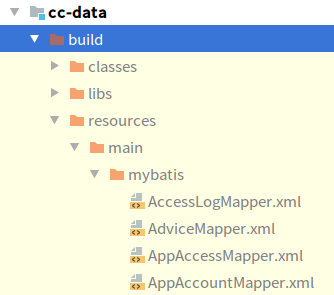
\includegraphics[scale=0.7]{classpathfile}
	\caption{MyBatis映射classpath中的文件}
	\label{fig:classpathfile}
\end{figure}

classpath是指编译过后的WEB-INF文件夹下的的classes目录。配置文件一般放在 resources 目录下, 当编译之后会自动复制到 classes 目录下。classpath*:的使用是为了多个component(最终发布成不同的jar包)并行开发,各自的bean定义文件按照一定的规则:package+filename,而使用这些component的调用者可以把这些文件都加载进来。不仅包含 classes 路径,还包括 jar 文件 classes 路径进行查找。classpath:只能加载找到的第一个文件。然而,使用classpath*:需要遍历所有的classpath,加载速度很慢,因此您应该尽量避免使用classpath*。有时提示找不到资源文件,首先检查资源文件夹的名称,资源文件夹的名称默认为resources,注意有一个s,其次是要检查此文件夹是否定义成了资源文件夹,资源文件夹与普通文件夹不同,资源文件夹有一个层叠的标识,如图\ref{fig:javaresourcefolder}所示。

\begin{figure}[htbp]
	\centering
	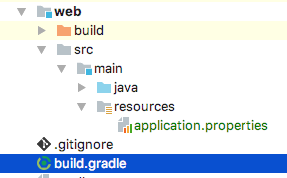
\includegraphics[scale=0.8]{javaresourcefolder.png}
	\caption{Intellij Idea中的资源文件夹}
	\label{fig:javaresourcefolder}
\end{figure}

仅仅是建立一个resources文件夹是不够的,还需要将之定义成资源文件夹,在文件夹上右键,选择Mark Directionary As,将之定义为资源文件夹。定义为资源文件夹后,即可通过如下方式指定配置文件的位置:

\begin{lstlisting}[language=Java]
@Configuration
@Data
@Component
@PropertySource("classpath:application.properties")
@ConfigurationProperties(prefix = "spring.datasource")
public class DataSourceConfig {

	private String jdbcUrl;
	
	private String username;
	
	private String driverClassName;
	
	private String password;
}
\end{lstlisting}

在Intellij Idea中,如果要把配置文件加入classpath,可以将配置文件标记为资源文件。

\subsection{Spring Boot开发者工具}

spring-boot-devtools为应用提供一些开发时特性,包括默认值设置,自动重启,livereload等。在build.gradle文件里添加开发工具配置:

\begin{lstlisting}[language=Bash]
compile "org.springframework.boot:spring-boot-devtools"
\end{lstlisting}

在激活了开发者工具后,Classpath里对文件做任何修改都会触发应用程序重启。为了让重启速度够快,不会修改的类(比如第三方JAR文件里的类)都加载到了基础类加载器里,而应用程序的代码则会加载到一个单独的重启类加载器里。检测到变更时,只有重启类加载器重启。在Intellij Idea中,需要在设置中配置Compiler,勾选上build project automatically选项。在Mac中,按下 command + alt + shift + / 出现的界面中,选择Registry。找到 “compiler.automake.allow.when.app.running” 这个选项,并且勾选。遗憾的是在自己的Mac中,Intellij Idea按照如上配置后还是不能正常自动Reload,不过当在点击了Reload Changed Classes之后,Spring Boot会自动重启,可以配置Reload Changed Classes的快捷键来实现。试用了发现,自动重启并不是很好用,有时重启会生效,有许多无效的重启,每次更改重启体验非常差。

\subsection{集合操作(Collection Operate)}

Java 8的stream可以像操作数据库那样操作内存,代码简洁清晰易懂,缺点是性能比传统处理方式较低。List移除空元素,移除重复元素:

\begin{lstlisting}[language=Java]
request.getParamList().stream()
		.filter(StringUtils::isNotEmpty)
		.distinct()
		.forEach(param -> {
			if (param.length() == 18 && CommonUtil.isLetterOrNumber(param)) {
			
			});
\end{lstlisting}

获取Json单个值:

\begin{lstlisting}[language=Java]
JSONObject json = new JSONObject(responseContent);
String total = json.getString("totalElementsCondition1");
\end{lstlisting}

去除List元素中的特殊字符:

\begin{lstlisting}[language=Java]
List<AccessLog> logs = operationLogs.stream()
		.peek(log -> log.setQueryResult(log.getQueryResult().replaceAll("\u0000", "")))
		.collect(Collectors.toList());
\end{lstlisting}

peek()-->对每个遇到的元素执行一些操作。如上方法会遍历List列表operationLogs中的每个元素,将特殊字符\textbackslash u0000去掉。

\paragraph{数组转换为ArrayList}

数组转List有如下方式:

\begin{lstlisting}[language=Java]
Integer[] integers = new Integer[] {1,2,3,4,5};
// Cannot modify returned list
List<Integer> list21 =  Arrays.asList(integers); 
// good
List<Integer> list22 = new ArrayList<>(Arrays.asList(integers)); 
//Java 8
List<Integer> list23 = Arrays.stream(integers).collect(Collectors.toList()); 
\end{lstlisting}

采用Arrays.asList转时,返回的List不能修改,因为asList()返回的列表是由原始数组支持的固定大小的列表。这种情况下,如果添加或删除列表中的元素,程序会抛出异常UnsupportedOperationException。

\paragraph{List分组}

如下代码片段按照responsekey对集合进行分组:

\begin{lstlisting}[language=Java]
Map<String, List<FeedbackRecord>> groupByLists = feedbackRecords.stream()
		.collect(Collectors.groupingBy(FeedbackRecord::getResponsekey));
\end{lstlisting}

如果需要在创建List时对其初始化:

\begin{lstlisting}[language=Java]
new ArrayList<String>() {{
	add(feedback.getResponsekey());
}}
\end{lstlisting}

有时需要将List对象按照对象某一个字段是否重复进行去重,可以先重写对象的equals方法:


\begin{lstlisting}[language=Java]
@Override
public boolean equals(Object o) {
	if (this == o) return true;
	if (!(o instanceof UnitedAwardsPenalties)) return false;
	UnitedAwardsPenalties stu = (UnitedAwardsPenalties) o;
	return implementContent != null ? implementContent.equals(stu.implementContent) : stu.implementContent == null;
}

@Override
public int hashCode() {
	int result = id.hashCode();
	result = 31 * result + memo.hashCode();
	return result;
}
\end{lstlisting}

就可以对对象进行直接比较:

\begin{lstlisting}[language=Java]
/**
* 去重
*/
unitedAPMapper.pageUnitedAPList(paramsMap)
				.stream()
				.forEach(element -> {
	if (!distinctUnitedAwardsPenaltiesList.contains(element)) {
		distinctUnitedAwardsPenaltiesList.add(element);
	}
});
\end{lstlisting}


\paragraph{查找}

如下代码片段查找第一个符合条件的元素:

\begin{lstlisting}[language=Java]
Optional<FeedbackRecord> filterFeedbackRecord = entry.getValue()
	.stream()
	.filter(feedbackRecord -> "0".equals(feedbackRecord.getIsFeedback()))
	.findFirst();
//更加直接的方式判断是否有符合条件的元素
boolean isChild = users.stream().anyMatch(t->t.age<18);
\end{lstlisting}

\paragraph{parallelStream}

在采用parallelStream时,不能使用全局的可变对象,要么使用不可变对象,要么使用局部对象,如下代码片段所示:

\begin{lstlisting}[language=Java]
List<String> example = new ArrayList<>();
example.add("a");
example.add("b");
example.add("c");
example.add("d");
Pageable pageable = DataUtils.pageable(1, 2, "a", "asc");
for (int i = 0; i < 10000; i++) {
	example.parallelStream().forEach(element -> {
		pageable.addSomeParam("a", element);
		if ("a".equals(element)) {
			System.out.println(pageable.getParams().get("a"));
		}
	});
}
\end{lstlisting}

运行此段代码,会发现和字符串a相等的元素输出有可能为b、c、d。为什么会出现这样的现象呢,是由于使用了全局的可变对象pageable,当执行到输出语句时,pageable可能已经被其他线程设置成了另外的值。解决的办法要么是把pageable做成不可变的对象,并只能在初始化的时候改变其内容,要么将之移动到局部,每次循环的时候创建新的pageable对象。

\subsection{正则表达式(Regular Expression)}

匹配电话号码的正则表达式:

\begin{lstlisting}
"^1(3[4-9]|4[7]|5[0-27-9]|7[08]|8[2-478])\\d{8}$"
\end{lstlisting}

[]匹配模式能够匹配方括号内任意字符,[08]可匹配0或者8。以上匹配电话号码的正则表达式会随着时间过期,比如某些号码段新开放时,相应的正则表达式会过期,比如以上正则表达式就无法匹配17623083674这个电话号码。

\subsection{Code Snippets}

有时想测试某段代码的运行效果,代码足够短也不太需要使用IDE来运行,相当于一个代码草稿本类似的功能。那么此时可以使用Visual Studio Code中使用Code Runner插件,此插件可以支持多种语言,测试草稿代码,如图\ref{fig:visualstudiocodesnippet}所示,想要查看对一个空字符串做toString()操作会有什么效果:

\begin{figure}[htbp]
	\centering
	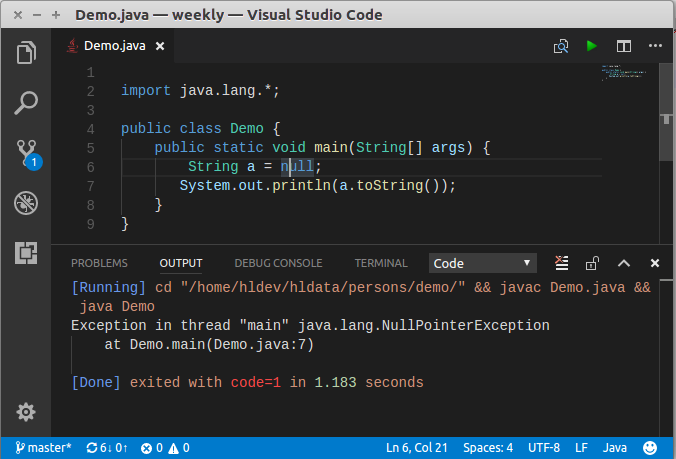
\includegraphics[scale=0.5]{visualstudiocodesnippet.png}
	\caption{Visual Studio Code代码草稿}
	\label{fig:visualstudiocodesnippet}
\end{figure}

ArrayList分页:

\begin{lstlisting}[language=Java]
return new Page<>(pageable, menuList.subList((page - 1) * size, page * size));
\end{lstlisting}

Optional避免空指针:

\begin{lstlisting}[language=Java]
public static String getChampionName(Competition comp) throws IllegalArgumentException {
	return Optional.ofNullable(comp)
		.map(c->c.getResult())
		.map(r->r.getChampion())
		.map(u->u.getName())
		.orElseThrow(()->new IllegalArgumentException("The value of param comp isn't available."));
}
\end{lstlisting}

Optional参数验证:

\begin{lstlisting}[language=Java]
public void setName(String name) throws IllegalArgumentException{
	this.name = Optional.ofNullable(name)
				.filter(User::isNameValid)
				.orElseThrow(()->new IllegalArgumentException("Invalid username."));
}
\end{lstlisting}


String.ValueOf()的坑:

\begin{lstlisting}[language=Java]
//如果article.getCategory()为空返回null字符串
String categoryId = String.valueOf(article.getCategory());
//养成字符串写前面比较的习惯
//避免空指针异常
if ("null".equals(categoryId)) {
	throw new HlValidateException(400001, "传入参数异常,栏目ID不能为空");
}
\end{lstlisting}

String.valueOf中如果对象为空,就返回字符串的"null",注意不是null对象,是字符串、字符串、字符串。常用启动命令:

\begin{lstlisting}[language=Bash]
#启动WebService
nohup /home/app/local/jdk1.8.0_111/bin/java -Xmx8192M -Xms4096M -jar -Xdebug -Xrunjdwp:transport=dt_socket,suspend=n,server=y,address=5010 /home/app/backend/api/credit-system-web-api-1.1.26.jar --spring.config.location=application-jjxxzx-test.properties>/dev/null &
#启动API
nohup /home/app/local/jdk1.8.0_111/bin/java -Xmx8192M -Xms4096M -jar -Xdebug  -Xrunjdwp:transport=dt_socket,suspend=n,server=y,address=5010  /home/app/backend/api/credit-system-web-api-1.1.26.jar  --spring.config.location=application-shuitu-api.properties>/dev/null &
\end{lstlisting}

dt表示Data Transport。-Xdebug是通知JVM工作在Debug模式下。-Xrunjdwp是通知JVM使用(Java Debug Wire Protocol)来运行调试环境。suspend指示是否在调试客户端建立起来后,再执行JVM。server参数是指是否支持在server模式的JVM中。


\paragraph{call to static DataFormat}

DateFormats是非线程安全:

\begin{lstlisting}[language=Java]
public static String format(Timestamp timestamp) {
	/**
	* DateFormats是非线程安全的
	* 每次调用创建新的对象
	*/
	return new SimpleDateFormat("yyyy-MM-dd HH:mm:ss").format(timestamp);
}
\end{lstlisting}

Method may fail to clean up stream or resource。这种方法可能无法清除(关闭,处置)一个流,数据库对象,或其他资源需要一个明确的清理行动。一般来说,如果一个方法打开一个流或其他资源,该方法应该使用try / finally块来确保在方法返回之前流或资源已经被清除了。


\section{接口(Application Interface)}

\subsection{请求消息(Request)}

HttpServletResponse对象(HttpServletRequest同理)的字符输出流在编码时,默认采用的是ISO 8859-1编码,该编码方式不兼容中文,比如会将"中国"编码为"63 63"(在ISO 8959-1的码表中查不到的字符会显示63)。当浏览器对接收到的数据进行解码时,会默认采用GB2312,将"63"解码为"?",浏览器就将"中国"两个字符解码为"??"。在获取请求消息记录日志时,获取到的汉字乱码。获取请求参数的语句为:

\begin{lstlisting}[language=Java]
// 获取未经过解码的参数(汉字会显示乱码)
String queryString = request.getQueryString();
// 获取经过解码的参数
String qymc = request.getParameter("qymc");
\end{lstlisting}

使用request.getParameter方式获得的参数是已经经过web服务器解码的。使用request.getQueryString可以获得未解码的原始参数。对于tomcat解码造成的乱码问题可以通过2种途径解决,修改tomcat配置文件设置解码方式,服务器端对于获取到的参数进行new String(param.getBytes("ISO-8859-1"),"页面指定编码")转换,如下代码片段所示:

\begin{lstlisting}[language=Java]
// 将获取到的消息解码
String decodedQueryString=new String(queryString.getBytes("ISO-8859-1"),"UTF-8");
\end{lstlisting}

\paragraph{POST请求}

发送POST请求时,客户端统一使用Json发送,服务端通过定义实体来获取。

\begin{lstlisting}[language=Java]
@PostMapping("create")
@ApiOperation(value = "创建文章", notes = "创建文章")
public ApiResult createArticle(@RequestBody Article article) {
}
\end{lstlisting}

@RequestBody需要把所有请求参数作为json解析,因此,不能包含key=value这样的写法在请求url中,所有的请求参数都是一个Json。使用curl模拟POST请求:

\begin{lstlisting}[language=Bash]
curl -X POST -H "APPID:hlb1451j6d136334gh2" \
-H "TIMESTAMP:2016-12-19 16 (tel:2016121916):58:02" \
-H "ECHOSTR:sdsaasf" \
-H "TOKEN:e02016ed4adfda9d9743ab70cf389ef9877c4a0e" \
-H 'Content-Type: application/json;charset=UTF-8' \
http://59.214.215.6:28080/api/article/create \
--data-binary $'{"title":"a123","content":"123456","category":12,"publisher":"ab"}'|jq '.'
\end{lstlisting}

需要传递请求头Content-Type,否则会提示如下错误:

\begin{lstlisting}
Content type 'application/x-www-form-urlencoded;charset=UTF-8' not supported
\end{lstlisting}

\paragraph{编辑请求(Edit Request)}

有时在写好接口之后,修改可能是非常细小的,比如原来的接口路径是/page,但是现在需要返回全部的数据可能就是/page/all(也可以在原来的接口方法改造,这里不考虑哪种方法实现更优)。需要测试一下新接口的返回,一种可以在浏览器的Network页中拷贝出curl请求命令来修改,修改后直接通过curl请求;一种方法在浏览器中安装tamper插件,抓取请求修改;一种方法可以使用Zed Attack Proxy\footnote{\url{https://github.com/zaproxy/zaproxy}}代理,在代理中选择Resend,在Resend界面中编辑HTTP请求信息。


\subsection{返回消息封装(Message Encapsulation)}

一个完整的标准化服务描述性语言SOAP(Simple Object Access Protocol,简单对象访问协议)在某些环境下表现的还不错。尽管如此,SOAP产品的性能开销很大,它是一个巨大的性能杀手。这也是Restful接口及接口采用Json交互的优势之一,在编写Restful接口时,需要将返回的内容用标准格式进行封装。通过编写统一的返回实体来实现:

\begin{lstlisting}[language=Java]
@RequestMapping("books")
public RestApiResponse<List<Book>> getUserShelfBooks(long userId){
	List<Book> userShelfBooks = bookShelfComposite.getUserShelfBooks(userId);
	return new RestApiResponse<>(ResponseCode.REQUEST_SUCCESS_MESSAGE, ResponseCode.REQUEST_SUCCESS, userShelfBooks);
}
\end{lstlisting}

RestApiResponse为统一定义的返回实体,所有的接口都会返回标准的RestApiResponse对象,对象通过泛型定义了不同的返回内容。

\paragraph{接口返回(Interface Response)}

接口返回的格式如图所示:

\begin{figure}[htbp]
	\centering
	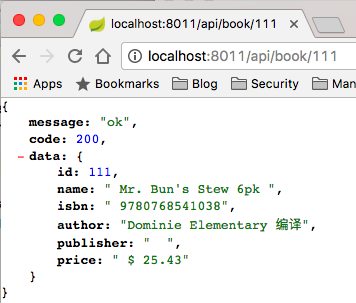
\includegraphics[scale=0.6]{restresponse.png}
	\caption{Restful接口返回数据示例}
	\label{fig:restresponse}
\end{figure}

其中,message可能缩写为mesg、msg等,为了避免歧义,没有使用缩写,也没有命名为errorMessage,是因为考虑到返回时不仅仅只有错误消息。针对不同的接口返回不同的字段,可以使用MapperFacade的Mapper方法进行映射,如下代码片段所示:

\begin{lstlisting}[language=Java]
@Autowired
private MapperFacade corporationMapperFacade;

public XydmResponse mapToCorporationResponse(Corporation corporation) {
return corporationMapperFacade.map(corporation, XydmResponse.class);
}
\end{lstlisting}

\subsection{接口认证(Authorization)}
\label{sec:authorization}

目前接口认证采用根据TIMESTAMP、ECHOSTR、APPKEY、APPID生成的Token,将之
发送到服务端,服务端采用同样的加密方式生成Token来进行比对认证。但是目前未做Token时间
过期判断,容易遭受重放攻击(Replay Attack\footnote{\url{https://en.wikipedia.org/wiki/Replay_attack}})。而且从流量中是可以轻松拿到请求头,对于专业选手来说,相当于大门敞开。采用如下Shell脚本\footnote{风格参考Google Shell风格指南:\url{http://zh-google-styleguide.readthedocs.io/en/latest/google-shell-styleguide/formatting/}}生成SHA1串。

\begin{lstlisting}[language=Bash]
# Mac生成sha256串
echo -n "foobar" | shasum -a 256
# Mac生成sha1串
echo -n "foobar" | shasum -a 1
readonly TOKEN = echo -n "foobar" | openssl dgst -sha256
\end{lstlisting}

脚本的目的是要使用不同的时间,随机生成的字符串,保证每次请求的Token都需要不一样,相当于一次一密。使用如下脚本生成随机token:

\begin{lstlisting}[language=Bash]
#!/bin/bash

#
# 认证请求脚本
# 根据时间戳生成请求,每次请求使用不同Token
# 避免重放攻击(Replay Attack)
# Author:
# 		dolphin
# Globals:
#   APP\_ID:
# Arguments:
#   None
# Returns:
#   接口调用返回结果
# TODO:根据不同的随机串排序,生成不同Toekn
#

readonly APP_ID="hlb1451j6d136334gh2"
readonly APP_KEY="test"

ECHOSTR=`head -n 1 /dev/urandom|sed 's/[^a-z0-9]//g'|md5sum|awk '{print $1}'`
CURRENT_TIME=`date '+%Y-%m-%d %H:%M:%S'`

#
# 生成TOKEN
# hlb1451j6d136334gh2接口各项认证参数的排列顺序是:
# 时间戳(timestamp)、AppKey、随机字符串(echostr)
# \$1接收来自命令行传入的参数
# 第二个参数用\$2接收,以此类推
# \$@表示所有的参数,相当于Java中main函数中定义的参数数组
#
SORTED_TOKEN=`echo -n ${CURRENT_TIME}_${APP_ID}_${APP_KEY}_${ECHOSTR}|tr '_' '\t'|sort|tr -d '\011'`
TOKEN=`echo -n ${APP_ID}${APP_KEY}${CURRENT_TIME}${CONST_STR}|md5sum|awk '{print $1}'`
SEQUENCE_TOKEN=`echo -n ${CURRENT_TIME}${APP_ID}${APP_KEY}${CONST_STR}|shasum -a 1|awk '{print $1}'`

# 请求服务端
COMMAND=`curl -H "APPID:$APP_ID" -H "TIMESTAMP:$CURRENT_TIME" -H "ECHOSTR:$CONST_STR" -H "TOKEN:$SEQUENCE_TOKEN" \
http://localhost:28080/api/blacklist/page?xdr= | jq '.'`
\end{lstlisting}

将APPID、APPKEY、时间戳,随机字符串采用SHA1加密后,生成Token发送给服务端,服务端再按照同样的步骤产生Token,两个Token进行比对,这里的关键是APPKEY只有服务端和客户端知道,其他非法用户不知道APPKEY,无法伪造Token。echo加上-n(newline)参数表示不换行输出。Linux中的随机数可以从两个特殊的文件中产生,一个是/dev/urandom.另外一个是/dev/random。他们产生随机数的原理是利用当前系统的熵池来计算出一定数量的随机比特,然后将这些比特作为字节流返回。熵池就是当前系统的环境噪音,熵指的是一个系统的混乱程度,系统噪音可以通过很多参数来评估,如内存的使用,文件的使用量,不同类型的进程数量等等。如果当前环境噪音变化的不是很剧烈或者当前环境噪音很小,比如刚开机的时候,而当前需要大量的随机比特,这时产生的随机数的随机效果就不是很好了。这就是为什么会有/dev/urandom和/dev/random这两种不同的文件,后者在不能产生新的随机数时会阻塞程序,而前者不会(ublock),当然产生的随机数效果就不太好了,这对加密解密这样的应用来说就不是一种很好的选择。/dev/random会阻塞当前的程序,直到根据熵池产生新的随机字节之后才返回,所以使用/dev/random比使用/dev/urandom产生大量随机数的速度要慢。


不过在接口中还多了一个排序的步骤,就是将APPID、APPKEY、时间戳,随机字符串按照一定的规则排序,因为随机字符串每次都是不同的,那么加密的APPID、APPKEY、时间戳,随机字符串顺序也会相应的发生变化。在Shell中,采用如下命令对APPID、APPKEY、时间戳,随机字符串进行排序:

\begin{lstlisting}[language=Bash]
# 测试排序语句
echo -n 'b a'|tr ' ' '\t' |sort|tr -d '\040\011\012\015'
# 实际排序语句
aSEQUENCE_TOKEN=`echo -n ${CURRENT_TIME}_${APP_ID}_${APP_KEY}_${CONST_STR}|tr '_' '\t'|sort|tr -d '\011'`
\end{lstlisting}

040表示空格,011表示制表符,012表示换行符(carriage returns),015表示新行(newlines)。最后的tr命令去掉排序后字符串中的制表符,这样排序后的语句就可以直接使用md5sum命令生成Token了。通过使用 tr,可以非常容易地实现 sed 的许多最基本功能。您可以将 tr 看作为 sed 的(极其)简化的变体:它可以用一个字符来替换另一个字符,或者可以完全除去一些字符。您也可以用它来除去重复字符。这就是所有 tr 所能够做的。-d参数表示删除(delete)。

\subsection{日志记录(Logging)}

接口日志记录时,自己的习惯是将之放在拦截器(Interceptor)中而不是单独写在方法中。写在方法里总有一些不可避免的重复,一旦修改起来许多地方都需要修改,而且非常容易遗漏。拦截器中缺点是无法很好的支持自定义日志的记录,而且对系统的性能等有影响。记录日志时需要获取响应Json的内容进行记录,通过反射获取。

\paragraph{获取Response返回内容}

在拦截器中记录日志时,有时需要获取HTTP Response中的内容,从图\ref{fig:outputchunkcontent}可以看出,只要获取到outputChunk的内容即可。

\begin{figure}[htbp]
	\centering
	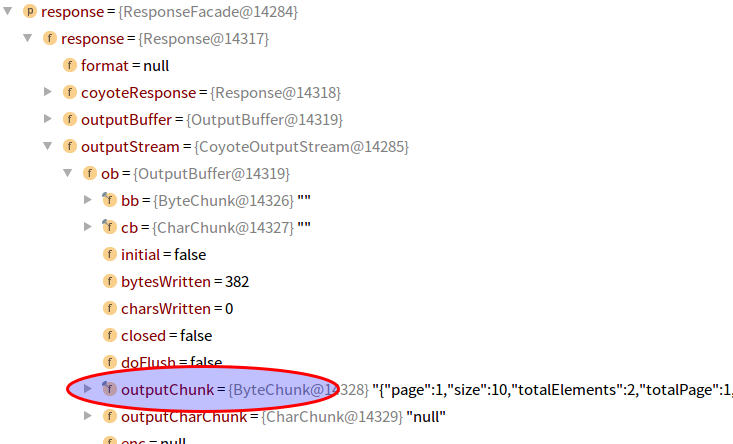
\includegraphics[scale=0.5]{outputchunkcontent.png}
	\caption{获取HTTP Response返回的内容}
	\label{fig:outputchunkcontent}
\end{figure}


可以通过反射来实现:

\begin{lstlisting}[language=Java]
public String getResponseContent(HttpServletResponse response) throws IOException, NoSuchFieldException, IllegalAccessException {
	String responseContent = null;
	CoyoteOutputStream outputStream = (CoyoteOutputStream) response.getOutputStream();
	Class<CoyoteOutputStream> coyoteOutputStreamClass = CoyoteOutputStream.class;
	Field obField = coyoteOutputStreamClass.getDeclaredField("ob");
	if (obField.getType().toString().endsWith("OutputBuffer")) {
		obField.setAccessible(true);
		OutputBuffer outputBuffer = (OutputBuffer) obField.get(outputStream);
		Class<OutputBuffer> opb = OutputBuffer.class;
		Field outputChunkField = opb.getDeclaredField("outputChunk");
		outputChunkField.setAccessible(true);
		if (outputChunkField.getType().toString().endsWith("ByteChunk")) {
			// 取到byte流
			ByteChunk bc = (ByteChunk) outputChunkField.get(outputBuffer);
			// 最终的值
			responseContent = new String(bc.getBytes(), "UTF-8");
		}
	}
	return responseContent;
}
\end{lstlisting}

OutputBuffer的命名空间为:org.apache.catalina.connector。在获取响应Json时,有时Json数据会比较长,一个无法避免的问题是只能获取到部分Json数据,那是因为在HTTP传输时,动态传输内容时,将返回内容以chunk的形式进行传输。HTTP 1.1时,Response要嘛通过Content-Length来指定要传输的内容大小,要嘛通过Transfer-Encoding: chunked来传输动态大小的内容,此时要求Response传输的内容要符合chunk encoding的规定。在交互式应用程序中有1个问题,就是它并不知道将要传输的数据有多大。在HTTP1.0中,服务器就会省略response头中的Content-Length而持续写数据出去,当服务器挂了的话,它简单地断开连接。而经典的HTTP客户端会一直读数据直到碰到-1(传输结束的标识符)。为了处理这个问题,HTTP1.1中增加了一个特殊的header:Transfer-Encoding:chunked,允许响应response被分块chunked。每次向连接写数据的时候会先计算大小,最后在response的尾部以一个0长度的chunk块标志着此次传输的结束。即HTTP1.1支持chunked编码,它允许HTTP消息被分成多块后再进行传输。Chunking一般用在服务器响应response的时候,但是客户端也可以chunk大的请求request。即Chunk编码允许服务器在发送完Header后,发送更多的Body内容。Chunked编码使用若干个Chunk块串连而成,每个Chunk块都以一个表明chunk快大小的16进制数字和一个额外的CRLF(回车换行)开始,后面跟着指定大小的内容。即每个Chunk块分为头部和正文两部分,头部内容指定下一段正文的字符总数(十六进制的数字)和数量单位(一般不写),正文部分就是指定长度的实际内容,两部分之间用回车换行(CRLF)隔开。最后以一个长度为0的Chunk表明本次传输结束。查看getOutputStream方法(在org.apache.catalina.connector命名空间下),代码如下:

\begin{lstlisting}[language=Java]
public ServletOutputStream getOutputStream() throws IOException {
	if (usingWriter) {
		throw new IllegalStateException(sm.getString("coyoteResponse.getOutputStream.ise"));
	}
	usingOutputStream = true;
	if (outputStream == null) {
		outputStream = new CoyoteOutputStream(outputBuffer);
	}
	return outputStream;
}
\end{lstlisting}

可以看出实际是从outputBuffer中取的内容,而outputBuffer的默认长度是8*1024(在OutputBuffer类下):

\begin{lstlisting}[language=Java]
public static final int DEFAULT_BUFFER_SIZE = 8*1024;
\end{lstlisting}

可以在preHandle中手动通过代码指定长度来解决这个问题:

\begin{lstlisting}[language=Java]
/**
* 在记录接口日志时
* 由于有时返回的内容过长,在getResponseContent通过反射获取到的只是一部分Json
* 导致后面Json解析失败
* 所以这里手动修改buffer的长度
* 使得一次能过获取较大的Json内容
* 不过当返回的Json内容超过2048 * 20时
* 同样只能获取部分
* 默认的长度是8*1024    public static final int DEFAULT_BUFFER_SIZE = 8*1024;
*/
response.setBufferSize(2048 * 20);
\end{lstlisting}

\subsection{异常处理(Exception Handle)}

在系统中,异常处理一般通过全局异常捕获,这样就几乎不用在代码中使用异常捕获块,过多的异常捕获代码块也会造成代码的污染和重复。在Spring中,可以在class注解上@ControllerAdvice来捕获全局异常:

\begin{lstlisting}[language=Java]
@ControllerAdvice(basePackages = "creditsystem.web.controllers")
public class CreditsystemControllerAdvice extends ResponseEntityExceptionHandler {

	@ExceptionHandler(HlValidateException.class)
	@ResponseBody
	ResponseEntity<?> handleValidateException(HttpServletRequest request, HlBaseException ex) {
		HttpStatus status = HttpStatus.OK;
		return new ResponseEntity<>(ApiResult.error(ex.getErrCode(), ex.getErrMsg(), ex.getData()), status);
	}
}
\end{lstlisting}

这样在业务逻辑层面遇到异常,只需要抛出异常即可,具体的异常处理流程由全局的异常处理模块来负责。以上代码还有一个问题,在添加了basePackages的扫描范围限制后,在拦截器中抛出异常时,全局异常处理类无法捕获异常。即使将拦截器的包空间加入到basePackages中也无效,暂时未找到原因。去掉basePackages的限制是可以捕获到异常的,这里捕获到异常时,接口返回标准的Json格式内容,这样调用方就方便解析并处理异常了。ExceptionHandler指定捕获的异常类型,不同的异常类型会进入到不同的方法来处理。

\subsection{版本管理(Interface Version Control)}

接口升级时,有的时候的修改是会影响到下游调用的,无法做到完全兼容,当升级了接口之后,原来的接口调用逻辑就无法正常使用了。所以,考虑做接口的版本管理,当发布接口时,发布一版新的接口,旧有的接口继续提供服务。升级接口由下游的用户来决定,这样在做不兼容升级时,不会影响原来的接口。

\paragraph{URI Parameter Versioning}

将Api的版本信息放到URI的参数里:

\begin{lstlisting}[language=HTML]
http://example.com/api/user?version=v1.1.30
\end{lstlisting}

这种方式被Amazon、Google、Netflix采用,流行度高。客户端可以通过指定参数选择调用服务端的Api版本,比如服务端提供v1、v2版本,当v1不可用时,可以在接口调用时指定v2版本的接口。项目也选用这种实现方式,后端部署多个版本对应部署多个服务,在Nginx中根据URL的传入参数路由到不同版本的服务上。

\begin{lstlisting}
server{
	location /api {
		if($query_string ~ version=v1.1.30){
			//如果query string中包含"version=v1.1.30"
			//流量转发到18081端口
			proxy_pass http://10.10.1.12:18081;
			proxy_redirect off;
		}else{
			proxy_pass http://10.10.1.12:18082;
			proxy_redirect off;
		}
	}
}
\end{lstlisting}

根据URL请求的版本参数路由到后端不同版本的服务。\$query\_string是Nginx的内置变量。$\sim$表示区分大小写到正则匹配,$\sim$*表示不区分大小写的正则匹配。


\paragraph{URI Versioning}

将Api的版本信息放到URI里:

\begin{lstlisting}[language=HTML]
http://example.com/api/v1.1.30/user
\end{lstlisting}

这种方式被Twitter、Facebook\footnote{\url{https://developers.facebook.com/docs/marketing-api/versions}}采用。

\paragraph{Header Versioning}

通过添加自定义请求头来指定Api的版本:

\begin{lstlisting}[language=HTML]
x-ms-version:2017-04-17
\end{lstlisting}

这种方式被Microsoft使用\footnote{\url{https://docs.microsoft.com/en-us/rest/api/storageservices/Versioning-for-the-Azure-Storage-Services?redirectedfrom=MSDN}}。

\subsection{接口缓存(Interface Cache)}

由于每次接口请求都需要调用认证信息,认证数据一旦生成,变动较少,所以将接口认证数据缓存。

\begin{lstlisting}
@Cacheable(value = "appAccount", key = "#id")
public Optional<AppAccount> findAppAccountById(String id){
	return Optional.ofNullable(appAccountMapper.findOne(id));
}
\end{lstlisting}

\section{数据库操作(Database Operate)}

\subsection{Could not get JDBC connection}

接口有时会查询不出数据,总是报超时错误。查看程序日志,提示Could not get JDBC Connection。查看了数据库的Session数量(40)远远未到达最大限制数量(500)。

\begin{lstlisting}[language=SQL]
#达梦DB查看最大会话数量
select *
from v$dm_ini
where para_name ='MAX_SESSIONS'

#达梦DB查看当前会话数量
SELECT count(*)
FROM v$sessions;
\end{lstlisting}

经过分析,是由于连接池的默认设置数量问题,由于配置中对HikariCP的连接池数量未做指定,HikariCP默认的连接池数量(maximumPoolSize)是10,正是由于连接池数量较小,很容易出现获取不到连接而出现超时的现象。This property controls the maximum size that the pool is allowed to reach, including both idle and in-use connections. Basically this value will determine the maximum number of actual connections to the database backend. A reasonable value for this is best determined by your execution environment. When the pool reaches this size, and no idle connections are available, calls to getConnection() will block for up to connectionTimeout milliseconds before timing out. Default: 10.如下配置HikariCP的连接池数量:

\begin{lstlisting}[language=Bash]
#
# Pool数太少会出现连接超时,Hikari默认的大小是10
# 用户数200-3000连接池目前设置为200
# 调大时综合服务器内存、CPU负荷进行考虑
# 数据库目前最大Session数量为500
#
spring.datasource.maximumPoolSize=200
\end{lstlisting}


\subsection{JDBC数据库重连(JDBC Database Reconnect)}

在数据库重启后,程序无法重新连接到数据库。程序使用的是Hikari,Hikari自带数据库重连机制。可以将连接池到c3p0,c3p0连接池本身具有数据库重连机制。目前常见到连接池如表\ref{table:databaseconnectionpool}所示:

\begin{table}
	\caption{常见数据库连接池}
	\label{table:databaseconnectionpool}
	\begin{center}
	\begin{tabular}{|c|c|p{7cm}|}
		\hline
		\multirow{1}{*}{名称}
		%\multirow{1}{c|}{名称}  
		& \multicolumn{1}{c|}{协议} 
		& \multicolumn{1}{c|}{备注}\\			
		\cline{1-3}
		c3p0 &  LGPL v.2.1  & C3P0是一个开源数据连接池,Hibernate3.0默认自带的数据连接池,性能比较稳定。\\
		\hline
		HikariCP & Apache 2.0 & Fast, simple, reliable. HikariCP is a "zero-overhead" production ready JDBC connection pool. At roughly 130Kb, the library is very light. \\
		\hline
		Druid & Apache 2.0 & Druid是Java语言中最好的数据库连接池。Druid能够提供强大的监控和扩展功能。 \\
		\hline
		DBCP & Apache 2.0 & DBCP(DataBase connection pool),是 apache 上的一个 java 连接池项目,也是 tomcat 使用的连接池组件。单独使用dbcp需要2个包:commons-dbcp.jar,commons-pool.jar \\
		\hline
		BoneCP & Apache 2.0 & 使用HikariCP替代\\
		\hline
	\end{tabular}	
	\end{center}
\end{table}


Tomcat 在 7.0 以前的版本都是使用 commons-dbcp 做为连接池的实现,但是 dbcp 饱受诟病,原因有:

\begin{itemize}
	\item{dbcp 是单线程的,为了保证线程安全会锁整个连接池}
	\item{dbcp 性能不佳}
	\item{dbcp 太复杂,超过 60 个类}
\end{itemize}

dbcp 使用静态接口,在 JDK 1.6 编译有问题
dbcp 发展滞后
因此很多人会选择一些第三方的连接池组件,例如 c3p0 , bonecp, druid。为此,Tomcat 从 7.0 开始引入一个新的模块:Tomcat jdbc pool。登陆服务器,使用命令查看正常的数据库连接:

\begin{lstlisting}[language=Bash]
lsof -i:5236
\end{lstlisting}

在程序启动时,并没有真正建立TCP连接。只有真正的接受到请求查询数据库时,程序才与数据库建立TCP连接。此处建立了10个TCP连接。而Hikari默认的最大连接池数量也为10个。如下配置设启连接池连接池时,初始建立的连接数量为5个:

\begin{lstlisting}
spring.datasource.initial-size=5
\end{lstlisting}

在Spring中配置数据源类型如下:

\begin{lstlisting}[language=XML]
<!-- 指定数据源类型 -->
spring.datasource.type=com.zaxxer.hikari.HikariDataSource
\end{lstlisting}

Hikari默认的数据源默认的连接池数量为10个,默认的数量在HikariConfig类中进行的设置。为什么修改Spring的Initial Size数量会影响Hikari的连接数量呢?如果不配置数据源,Spring Boot默认的数据源是:

\begin{lstlisting}
org.apache.tomcat.jdbc.pool.DataSource
\end{lstlisting}

但是在实际开发中,可能需要使用自己是熟悉的数据源或者其他性能比较高的数据源。此时就可以通过制定Spring的数据源类型来实现。

停止数据库:

\begin{lstlisting}[language=Bash]
nohup sudo /opt/dmdbms/bin/dmserver /opt/dmdbms/data/DAMENG/dm.ini -noconsole &
\end{lstlisting}

在反复研究后发现,程序并未使用HikariCP连接池,而是使用的Spring JDBC连接池,所以在初始化Datasource时指定连接池,如下代码片段所示:

\begin{lstlisting}[language=Java]
@Configuration
@Data
@ConfigurationProperties(prefix = "spring.datasource")
public class DataSourceConfig {

	private String jdbcUrl;
	
	private String username;
	
	private String driverClassName;
	
	private String password;
	
	@Bean
	@Primary
	public DataSource primaryDataSource() {
		HikariConfig hikariConfig = new HikariConfig();
		hikariConfig.setDriverClassName(driverClassName);
		hikariConfig.setJdbcUrl(jdbcUrl);
		hikariConfig.setUsername(username);
		hikariConfig.setPassword(password);
		hikariConfig.setMaximumPoolSize(5);
		hikariConfig.setConnectionTestQuery("SELECT 1");
		hikariConfig.setPoolName("springHikariCP");
		hikariConfig.addDataSourceProperty("dataSource.cachePrepStmts", "true");
		hikariConfig.addDataSourceProperty("dataSource.prepStmtCacheSize", "250");
		hikariConfig.addDataSourceProperty("dataSource.prepStmtCacheSqlLimit", "2048");
		hikariConfig.addDataSourceProperty("dataSource.useServerPrepStmts", "true");
		HikariDataSource dataSource = new HikariDataSource(hikariConfig);
		return dataSource;
	}
}
\end{lstlisting}

\subsection{HikariCP数据库连接}

在配置HikariCP数据库连接时,总是提示如下错误:

\begin{lstlisting}
org.springframework.beans.factory.BeanCreationException: Error creating bean with name 'dataSource' defined in class path resource [org/springframework/boot/autoconfigure/jdbc/DataSourceConfiguration$Hikari.class]: Bean instantiation via factory method failed; nested exception is org.springframework.beans.BeanInstantiationException: Failed to instantiate [com.zaxxer.hikari.HikariDataSource]: Factory method 'dataSource' threw exception; nested exception is java.lang.NullPointerException
\end{lstlisting}

经过源码跟踪,发现是url为空导致的这个问题,后来增加了url的配置才得以成功连接数据库。所以除了要定义jdbc-url外,还需要定义url。经过查看HikariCP的文档,属性jdbc-url将使 HikariCP 使用“基于驱动管理器”(DriverManager-based)的配置。一般情况下,基于数据源(DataSource-based)的配置是更好的选择。但对许多部署实例来讲却也区别不大。当使用jdbc-url来配置“旧”的 JDBC 驱动时,你可能也需要设置 driverClassName 属性,但可以试一试不设置是否能行得通。所以,最终连接数据库的配置如下:

\begin{lstlisting}
spring.datasource.hikari.jdbc-url=jdbc:mysql://10.0.0.14:3306/dolphin
spring.datasource.hikari.url=jdbc:mysql://10.0.0.14:3306/dolphin
spring.datasource.hikari.username=root
spring.datasource.hikari.password=dolphin
spring.datasource.hikari.type=com.zaxxer.hikari.HikariDataSource
spring.datasource.hikari.driver-class-name=com.mysql.jdbc.Driver
\end{lstlisting}


\paragraph{DataSource跟DriverManager区别及联系}

In basic terms, a data source is a facility for storing data. It can be as sophisticated as a complex database for a large corporation or as simple as a file with rows and columns. A data source can reside on a remote server, or it can be on a local desktop machine. Applications access a data source using a connection, and aDataSource object can be thought of as a factory for connections to the particular data source that theDataSource instance represents.

两者相同点:
Using a DataSource object is the preferred alternative to using the DriverManager for establishing a connection to a data source. They are similar to the extent that the DriverManager class and DataSource interface both have methods for creating a connection, methods for getting and setting a timeout limit for making a connection, and methods for getting and setting a stream for logging.

两者不同点:
1.Unlike the DriverManager, a DataSource object has properties that identify and describe the data source it represents. Also, a DataSource object works with a JavaTM Naming and Directory InterfaceTM (JNDI) naming service and is created, deployed, and managed separately from the applications that use it. A driver vendor will provide a class that is a basic implementation of the DataSource interface as part of its JDBC 2.0 or 3.0 driver product.

2.The second major advantage is that the DataSource facility allows developers to implement a DataSourceclass to take advantage of features like connection pooling and distributed transactions.

传统的数据库连接方式(指通过DriverManager和基本实现DataSource进行连接)中,一个数据库连接对象均对应一个物理数据库连接,数据库连接的建立以及关闭对系统而言是耗费系统资源的操作,在多层结构的应用程序环境中这种耗费资源的动作对系统的性能影响尤为明显。

在多层结构的应用程序中通过连接池(connection pooling)技术可以使系统的性能明显得到提到,连接池意味着当应用程序需要调用一个数据库连接的时,数据库相关的接口通过返回一个通过重用数据库连接来代替重新创建一个数据库连接。通过这种方式,应用程序可以减少对数据库连接操作,尤其在多层环境中多个客户端可以通过共享少量的物理数据库连接来满足系统需求。通过连接池技术Java应用程序不仅可以提高系统性能同时也为系统提高了可测量性。

数据库连接池是运行在后台的而且应用程序的编码没有任何的影响。此中状况存在的前提是应用程序必须通过DataSource对象(一个实现javax.sql.DataSource接口的实例)的方式代替原有通过DriverManager类来获得数据库连接的方式。一个实现javax.sql.DataSource接口的类可以支持也可以不支持数据库连接池,但是两者获得数据库连接的代码基本是相同的。

\subsection{Spring Boot缓存}

SpringBoot支持很多种缓存方式:redis、guava、ehcahe、jcache等等。出现At least one cache should be provided per cache operation错误时,表示没有指定Cache缓存框架,需要在XML中配置。EhCache 是一个纯Java的进程内缓存框架,具有快速、精干等特点,是Hibernate中默认的CacheProvider。ehcache提供了多种缓存策略,主要分为内存和磁盘两级,所以无需担心容量问题。

@Cacheable : Spring在每次执行前都会检查Cache中是否存在相同key的缓存元素,如果存在就不再执行该方法,而是直接从缓存中获取结果进行返回,否则才会执行并将返回结果存入指定的缓存中。 

@CacheEvict : 清除缓存。 

@CachePut : @CachePut也可以声明一个方法支持缓存功能。使用@CachePut标注的方法在执行前不会去检查缓存中是否存在之前执行过的结果,而是每次都会执行该方法,并将执行结果以键值对的形式存入指定的缓存中。 

这三个方法中都有两个主要的属性:value 指的是 ehcache.xml 中的缓存策略空间;key 指的是缓存的标识,同时可以用 \# 来引用参数。
在ehcache.xml中配置缓存策略空间:

\begin{lstlisting}[language=XML]
<ehcache>
	<cache name="summaryXzxk" maxBytesLocalHeap="1m" timeToLiveSeconds="200"/>
</ehcache>
\end{lstlisting}

在方法上指定缓存,语法采用SpEL(Spring Express Language),Spring表达式语言全称为Spring Expression Language(缩写为SpEL),能在运行时构建复杂表达式、存取对象图属性、对象方法调用等等,并且能与Spring功能完美整合,如能用来配置Bean定义。 表达式语言给静态Java语言增加了动态功能。
SpEL是单独模块,只依赖于core模块,不依赖于其他模块,可以单独使用。:

\begin{lstlisting}[language=Java]
@Cacheable(value = "summaryXzxk",
key = "'findPage'+#pageable.page+#pageable.params.get('xdr')",
condition = "#pageable.params.get('xdr') eq null or #pageable.params.get('xdr') eq ''"
)
\end{lstlisting}

@Cacheable注解有三个参数,value是必须的,还有key和condition。第一个参数,也就是value指明了缓存将被存到什么地方。其中summaryXzxk为定义在配置文件中的缓存器名称。缓存的Key,当我们没有指定该属性时,Spring将使用默认策略生成key(表示使用方法的参数类型及参数值作为key),key属性是用来指定Spring缓存方法的返回结果时对应的key的。该属性支持SpringEL表达式。我们还可以自定义策略:自定义策略是指我们可以通过Spring的EL表达式来指定我们的key。这里的EL表达式可以使用方法参数及它们对应的属性。使用方法参数时我们可以直接使用“\#参数名”或者“\#p参数index”。key的生成策略有两种:一种是默认策略,一种是自定义策略。默认的key生成策略是通过KeyGenerator生成的,其默认策略如下:1.如果方法没有参数,则使用0作为key。2.如果只有一个参数的话则使用该参数作为key。3.如果参数多余一个的话则使用所有参数的hashCode作为key满足一定条件才缓存,写法如下:

\begin{lstlisting}[language=Java]
condition = "#pageable.params.get('xdr') eq null or #pageable.params.get('xdr') eq ''"
\end{lstlisting}

如上条件,取出xdr为空的数据进行缓存。如下情形缓存将会不起作用:

\begin{itemize}
	\item{同一个bean内部方法调用,这个问题遇到过,也是查了一些时间才发现}
	\item{子类调用父类中有缓存注解的方法}
\end{itemize}



\subsection{用户重复登录问题}

在服务端维护登录用户与其SessionID的对应关系。同一用户,后登陆者将前登陆者的SessionID替换,这样,前者如果再请求服务器资源,无法与新生成的Session ID匹配,此时服务端会返回一个错误码,前端捕获到此错误码,就会认为其未登录,要求重新登录。这样,即使出现断电等无法注销的情况,也会在他下次登陆时自动取代掉,同时也解决了用户登陆的唯一性问题。

\subsection{读取properties属性}

\paragraph{读取自定义属性}

有时需要读取自定义属性,以配置HikariCP连接池为例,在application.properties文件指定指定配置:

\begin{lstlisting}
spring.datasource.hikari.jdbc-url=jdbc:dm://dn4:5236/DMSERVER
\end{lstlisting}

在类中获取配置相应的值,注意需要添加Data注解,否则需要手写get和set方法:

\begin{lstlisting}[language=Java]
@Configuration
@Data
@ConfigurationProperties(prefix = "spring.datasource.hikari")
public class DataSourceConfig {
	private String jdbcUrl;
}
\end{lstlisting}

由于此处注解是默认写在application.properties配置文件中,所以在ConfigurationProperties中可以不指定路径。否则需要使用locations指定配置文件路径。

\section{单元测试(Unit Test)}

\subsection{Gradle中执行单元测试}

项目使用Gradle进行构建,写好单元测试类后,在Gradle中做如下配置:

\begin{lstlisting}[language=Java]
project(':cc-api') {	
	test{
		include('**/*Test.class')
	}
}
\end{lstlisting}

在每次构建时都会运行单元测试。Mock和Stub是两种测试代码功能的方法。Mock测重于对功能的模拟。Stub测重于对功能的测试重现。比如对于List接口,Mock会直接对List进行模拟,而Stub会新建一个实现了List的TestList,在其中编写测试的代码。强烈建议优先选择Mock方式,因为Mock方式下,模拟代码与测试代码放在一起,易读性好,而且扩展性、灵活性都比Stub好。

\subsection{TestNG单元测试}

项目经常涉及到修改,水平不够足,有些地方始终考虑的不够周到,会互相影响,所以考虑添加单元测试。系统前后端分离,分为各类接口,根据不同类的接口分组进行测试。在测试类上指定测试接口的分组:

\begin{lstlisting}[language=Java]
/**
* 组名是数组类型,,所以一个测试方法可以属于多个组
* group={"group name 1","group name 2"}
*/
@Test(groups = "xycq-api")
public void testGetXzcfList() throws Exception {
	TestPublicVariable.test("/xzcf?xdr=dolphin");
}
\end{lstlisting}

配置跑单元测试如图\ref{fig:testngunittestbygroup}所示。

\begin{figure}[htbp]
	\centering
	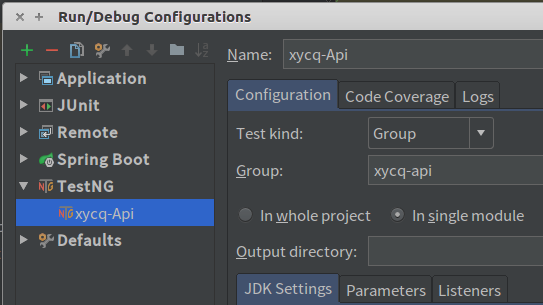
\includegraphics[scale=0.5]{testngunittestbygroup.png}
	\caption{TestNG单元测试}
	\label{fig:testngunittestbygroup}
\end{figure}

\subsection{Spring mockMvc测试}

MockMvc实现了对Http请求的模拟,能够直接使用网络的形式,转换到Controller的调用,这样可以使得测试速度快、不依赖网络环境,而且提供了一套验证的工具,这样可以使得请求的验证统一而且很方便。引入在Gradle构建脚本中增加Spring测试包:

\begin{lstlisting}
compile("org.springframework.boot:spring-boot-test:" + springBootVersion)
testCompile group: 'junit', name: 'junit', version: '4.12'
\end{lstlisting}

增加测试类:

\begin{lstlisting}[language=Java]
@RunWith(SpringRunner.class)
@SpringBootTest(classes = DolphinApplication.class)
@Commit
@Transactional
public class BookControllerTest {

	private MockMvc mockMvc;
	
	@Autowired
	private WebApplicationContext wac;
	
	@Before
	public void setUp() {
		this.mockMvc = webAppContextSetup(this.wac).build();
	}
	
	@Test
	public void getBooksByName() throws Exception {
		String responseString = mockMvc.perform(
										get("/api/book?name=小学生")
										).andExpect(status().isOk())    
										.andDo(print())         
										.andReturn().getResponse().getContentAsString();
		System.out.println("--------返回的json = " + responseString);
	}
}
\end{lstlisting}


\section{常见问题(Frequently Encounted Question)}

\paragraph{getAttribute: Session already invalidated}

当用户多次登录后,由于服务端缓存了所有的Session,在取出Session进行对比的时候,会出现此错误,此错误指示从Session中获取属性值的时候,Session已经无效。有两种可能导致Session无效:session timeout或者程序中调用了session.invalidate()方法。检查代码发现,在移除Session时的确使用了:

\begin{lstlisting}[language=Java]
// 使Session无效的语句
getSessionMap().get(sessionId).invalidate();
// 出错的语句
User user = (User) session.getAttribute("LOCAL_CLINET_USER");
\end{lstlisting}

当在无效的session中获取Attribute时,出现了上面的错误,解决办法就是不调用invalidate方法。

\paragraph{java.lang.NoClassDefFoundError: org/apache/juli/logging/LogFactory}

Tomcat 的内部日志使用 JULI 组件,这是一个 Apache Commons 日志的重命名的打包分支,默认被硬编码,使用 java.util.logging 架构。这能保证 Tomcat 内部日志与 Web 应用的日志保持独立,即使 Web 应用使用的是 Apache Commons Logging。在Gradle构建脚本中添加如下配置即可:

\begin{lstlisting}[language=Bash]
dependencies{
	compile group: 'org.apache.tomcat', name: 'tomcat-juli', version: property('tomcat.version')
}
\end{lstlisting}

连接时从内存找不到需要的class就出现NoClassDefFoundError,当Java虚拟机或 ClassLoader实例试图在类的定义中加载(作为通常方法调用的一部分或者作为使用 new 表达式创建的新实例的一部分),但无法找到该类的定义时,抛出此异常。 

Java事务的类型有三种:JDBC事务、JTA(Java Transaction API)事务、容器事务。 常见的容器事务如Spring事务,容器事务主要是J2EE应用服务器提供的,容器事务大多是基于JTA完成,这是一个基于JNDI的,相当复杂的API实现。在本机请求会报此错误,但是部署到服务器上是OK的。在本地引入如下2个jar包即可修复此问题:

\begin{lstlisting}[language=Bash]
compile group: 'javax.transaction', name: 'jta', version: '1.1'
compile group: 'ma.glasnost.orika', name: 'orika-core', version: '1.5.1'
\end{lstlisting}

Orika是一个Java Bean映射框架递,递归复制数据从一个对象到另一个。对于开发多层应用程序时,非常有用。Java 事务编程接口(JTA:Java Transaction API)和 Java 事务服务 (JTS;Java Transaction Service) 为 J2EE 平台提供了分布式事务服务。分布式事务(Distributed Transaction)包括事务管理器(Transaction Manager)和一个或多个支持 XA 协议的资源管理器 ( Resource Manager )。我们可以将资源管理器看做任意类型的持久化数据存储;事务管理器承担着所有事务参与单元的协调与控制。JTA 事务有效的屏蔽了底层事务资源,使应用可以以透明的方式参入到事务处理中;但是与本地事务相比,XA 协议的系统开销大,在系统开发过程中应慎重考虑是否确实需要分布式事务。若确实需要分布式事务以协调多个事务资源,则应实现和配置所支持 XA 协议的事务资源,如 JMS、JDBC 数据库连接池等。如果是引用包里面的类的路径找不到(例如:org/Spring/Application),那么就可以先查看项目的CLASSPATH是否包含引用包的路径:

\begin{lstlisting}[language=Java]
//打印项目的CLASSPATH
ClassLoader classLoader = ClassLoader.getSystemClassLoader();
URL[] urls = ((URLClassLoader) classLoader).getURLs();
for (URL url : urls) {
	System.out.println(url.getFile());
}
\end{lstlisting}

可以看到CLASSPATH路径里面没有包含引用包的路径,所以会提示找不到类。

\paragraph{no Scala SDK found in module}

项目编译的时候提示module里没有找到Scala SDK,因为module没有指定Scala SDK(或者是原来的配置由于某种原因实效了)。此时可以将Scala SDK添加到指定module里,File->Project Structure->Project Settings->Modules,在对应的module上右键添加Scala SDK,如图\ref{fig:addscalasdk}所示。

\begin{figure}[htbp]
	\centering
	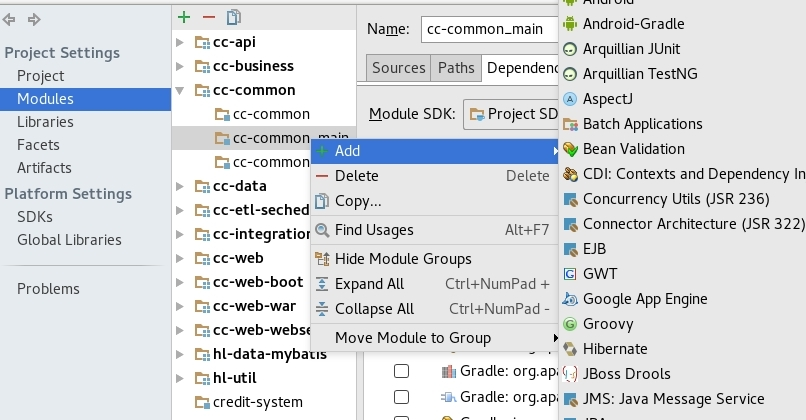
\includegraphics[scale=0.5]{addscalasdk.jpg}
	\caption{Intellij Idea中添加Scala SDK}
	\label{fig:addscalasdk}
\end{figure}

添加了Scala SDK后,编译的时候就可以编译module里面的scala文件了。

\paragraph{Unregistering JMX-exposed beans on shutdown}

运行之后控制台输出“Unregistering JMX-exposed beans on shutdown”,原因为:SpringBoot内置Tomcat没有正常启动.原来是在引入时没有写版本号,在没有版本号的情况下此次引入其实是不成功的,难怪在类中始终不能够自动导入对应的命名空间。

\begin{lstlisting}[language=Bash]
compile('org.springframework.boot:spring-boot-starter-web:1.5.2.RELEASE')
\end{lstlisting}

忘记了写:1.5.2.RELEASE,其实这里的版本号可以省略(应该是不能省略才是),但是目前还不清楚具体的省略机制,在什么情况下可以省略。

\paragraph{AES加密失败}

因为某些国家的进口管制限制,Java发布的运行环境包中的加解密有一定的限制。比如默认不允许256位密钥的AES加解密,解决方法就是修改策略文件。将下载的没有限制的文件替换掉原来的文件即可。替换的路径为:

\begin{lstlisting}[language=Bash]
/home/hl/local/jdk1.8.0_144/jre/lib/security/local_policy.jar
/home/hl/local/jdk1.8.0_144/jre/lib/security/US_export_policy.jar
\end{lstlisting}

由于信息安全在军事等方面极其重要,如在第二次世界大战期间,使用了无线电,若是能够成功解密敌方的机密情报,往往预示着战争的胜利,因此美国对加密解密等软件进行了出口限制,JDK中默认加密的密钥长度较短,加密强度较低,而UnlimitedJCEPolicyJDK7中的文件则没有这样的限制,因此为了获得更好的加密强度,需要替换掉那两个文件。如何知道文件是否已经替换成了允许256位加密的那个文件呢?只需要看文件的MD5即可,在Mac下:

\begin{lstlisting}[language=Bash]
# 切换到需要替换的文件所在目录
/Library/Java/JavaVirtualMachines/jdk1.8.0_112.jdk/Contents/Home/jre/lib/security/
# 查看文件的MD5编码
# 前提是需要知道替换后的那个文件的MD5编码
# 与当前生成的MD5编码的文件比对即可
MD5 local_policy.jar
# 在Ubuntu下使用此命令查看MD5
md5sum local_policy.jar
\end{lstlisting}

\subsection{java.lang.OutOfMemoryError: Java heap space	}

内存溢出是指应用系统中存在无法回收的内存或使用的内存过多,最终使得程序运行要用到的内存大于虚拟机能提供的最大内存。看到heap相关的时候就肯定是堆栈溢出了,此时如果代码没有问题的情况下,适当调整-Xmx和-Xms是可以避免的,不过一定是代码没有问题的前提,为什么会溢出呢,要么代码有问题,要么访问量太多并且每个访问的时间太长或者数据太多,导致数据释放不掉,因为垃圾回收器是要找到那些是垃圾才能回收,这里它不会认为这些东西是垃圾,自然不会去回收了;主意这个溢出之前,可能系统会提前先报错关键字为:

\begin{lstlisting}
java.lang.OutOfMemoryError:GC overhead limit exceeded
\end{lstlisting}

这种情况是当系统处于高频的GC状态,而且回收的效果依然不佳的情况,就会开始报这个错误,这种情况一般是产生了很多不可以被释放的对象,有可能是引用使用不当导致,或申请大对象导致,但是java heap space的内存溢出有可能提前不会报这个错误,也就是可能内存就直接不够导致,而不是高频GC。JVM在启动的时候会自动设置Heap size的值,其初始空间(即-Xms)是物理内存的1/64,最大空间(-Xmx)是物理内存的1/4。可以利用JVM提供的-Xmn -Xms -Xmx等选项可进行设置。例如:

\begin{lstlisting}[language=Bash]
nohup $JAVA_HOME/bin/java -Xmx8192M -Xms4096M -jar \
-Xdebug -Xrunjdwp:transport=dt_socket,suspend=n,server=y,address=5006 \
$APP_PATH/credit-system-web-api-$VERSION.jar \
--spring.config.location=application-api.properties>/dev/null &
\end{lstlisting}

以上启动项设置初始( initial size)Heap Size(Xms)是4096MB最大空间xmx(maximum size)8192MB。一种查明方法是不间断地监控GC的活动,确定内存使用量是否随着时间增加。如果确实如此,就可能发生了内存泄漏。如果发生了内存泄漏,可以使用JMap生成dump文件以供分析:

\begin{lstlisting}[language=Bash]
jmap -dump:format=b,file=heap.bin <pid> 
\end{lstlisting}

此种方式在执行时,JVM是暂停服务的,所以对线上的运行会产生影响。也可以在启动参数上设置发生OutOfMemory时生成dump文件:

\begin{lstlisting}[language=Bash]
# 发生OOM时生成dump文件
# 标准参数(-)
# 所有的JVM实现都必须实现这些参数的功能,而且向后兼容;
# 非标准参数(-X)
# 默认jvm实现这些参数的功能
# 但是并不保证所有jvm实现都满足,且不保证向后兼容;
# 非Stable参数(-XX)
# 此类参数各个jvm实现会有所不同,将来可能会随时取消
# 需要慎重使用;
-XX:+HeapDumpOnOutOfMemoryError
# dump文件存放路径
-XX:HeapDumpPath=/home/app
\end{lstlisting}

一般说来,一个正常的系统在其运行稳定后其内存的占用量是基本稳定的,不应该是无限制的增长的。同样,对任何一个类的对象的使用个数也有一个相对稳定的上限,不应该是持续增长的。根据这样的基本假设,我们持续地观察系统运行时使用的内存的大小和各实例的个数,如果内存的大小持续地增长,则说明系统存在内存泄漏,如果特定类的实例对象个数随时间而增长(就是所谓的“增长率”),则说明这个类的实例可能存在泄漏情况。

\section{MyBatis}

mybatis-spring-boot-starter 1.3.x版本对应Spring Boot 1.5.x版本。


\subsection{打印SQL(Print SQL)}

开发中,配置日志中打印SQL语句,在application.properties文件中指定mybatis配置文件路径:

\begin{lstlisting}[language=Bash]
mybatis.config-location=classpath:mybatis-config.xml
\end{lstlisting}

在Mybatis配置文件mybatis-config.xml中,做如下配置:

\begin{lstlisting}[language=XML]
<?xml version="1.0" encoding="UTF-8"?>
<!DOCTYPE configuration
PUBLIC "-//mybatis.org//DTD Config 3.0//EN"
"http://mybatis.org/dtd/mybatis-3-config.dtd">
<configuration>
	<settings>
		<!-- 打印查询语句 -->
		<setting name="logImpl" value="STDOUT_LOGGING" />
	</settings>
</configuration>
\end{lstlisting}

打印SQL语句效果如图\ref{fig:mybatisprintsql}所示。

\begin{figure}[htbp]
	\centering
	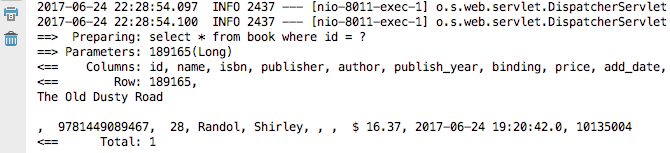
\includegraphics[scale=0.5]{mybatisprintsql.png}
	\caption{MyBatis打印SQL}
	\label{fig:mybatisprintsql}
\end{figure}

\subsection{多数据源(Multi-Datasource)}

项目开始的时候是将日志写在主数据库中,过程中考虑到数据库到压力,决定将日志单独放在另一台数据库中。目前还没有到需要使用MQ到程度。项目中数据持久化使用的是MyBatis,所以此时就需要配置MyBatis的多数据源支持。多数据源可以采用AOP动态切换的方式来实现。一种最简便的方式是初始化多个数据源,在创建jdbcTemplate实例时指定某个数据源即可,如下代码片段所示:

\begin{lstlisting}[language=Java]
@Autowired
@Qualifier("secondaryJdbcTemplate")
private JdbcTemplate jdbcTemplate1;
\end{lstlisting}

那么采用jdbcTemplate1执行的SQL都在数据源secondaryJdbcTemplate上操作,不过麻烦的地方是需要手动写SQL,但是由于有时采用的Mapper操作的数据库,如果可以直接通过注解来指定数据源岂不更加方便。如下是采用自定义注解 + AOP的方式实现数据源动态切换。
动态数据源能进行自动切换的核心就是spring底层提供了AbstractRoutingDataSource类进行数据源的路由的,我们主要继承这个类,实现里面的方法即可实现我们想要的,这里主要是实现方法:determineCurrentLookupKey(),而此方法只需要返回一个数据库的名称即可,所以我们核心的是有一个类来管理数据源的线程池,这个类才是动态数据源的核心处理类。还有另外就是我们使用AOP技术在执行事务方法前进行数据源的切换。



\subsection{多参数传递(Multi-Parameter)}

在使用Mybatis的过程中,有时需要传递多个参数,例如既要传入机构ID列表,又要传入其他参数,那么此时Mapper如下:

\begin{lstlisting}[language=Java]
int batchUpdate(@Param("ids") List<String> ids,@Param("status") String status);
\end{lstlisting}

在XML中使用:

\begin{lstlisting}[language=XML]
<update id="batchUpdate" parameterType="java.util.List">
	UPDATE TD_S_ORG
	SET STATUS = #{status}
	WHERE ORG_ID IN
	<foreach collection="ids" item="item" index="index" open="(" separator="," close=")">
		#{item}
	</foreach>
</update>
\end{lstlisting}

\subsection{批量写入}

在导入Excel的过程中,可以利用批量写入功能。可以使写入速度得到质的提高。批量写入在MyBatis中作如下配置:

\begin{lstlisting}[language=SQL]
<insert id="createBatch" parameterType="system.data.model.Reporting">
	insert into TI_B_XZXK_REPORTING (
		ID,
		SFGK,
		BGKYY
	) values
	<foreach collection="list" item="item" index="index" separator=",">
	(
		#{item.id},
		#{item.sfgk},
		#{item.bgkyy}
	)
	</foreach>
</insert>
\end{lstlisting}

参数传入List即可,注意列表的数量不宜过大,一般数据库对传入的参数有限制,也就是同时一批写入的数据量不能太大。

\subsection{resultMap和resultType区别}

使用resultType进行输出映射,只有查询出来的列名和pojo中的属性名一致,该列才可以映射成功。如果查询出来的列名和pojo中的属性名全部不一致,没有创建pojo对象。只要查询出来的列名和pojo中的属性有一个一致,就会创建pojo对象。mybatis通过resultMap能帮助我们很好地进行高级映射。遇到一个问题是将分页的本应该写成resultMap的地方写成了resultType,在本地可以正常运行,但是打包成jar包放到服务器就无法运行了,提示org.apache.ibatis.type.TypeException: Could not resolve type alias 'AccessLog':

\begin{lstlisting}[language=XML]
<!--这里的resultType应该写成resultMap-->
<select id="countAccessLog" parameterType="com.hualongdata.data.mybatis.Pageable" resultType="AccessLog">
</select>
\end{lstlisting}

如果改为resultMap又会出现如下错误:


\begin{lstlisting}[language=XML]
org.apache.ibatis.builder.IncompleteElementException: Could not find result map creditsystem.data.mapper.RedBalckLogMapper.RedBalckLog
\end{lstlisting}

出现这个错误的原因是在resultMap里面指定的是RedBalckLog(大写),而Mapper中定义的是redBalckLog(小写)。这里resultMap指定的Bean需要和Mapper文件中定义的Bean的id一致。

\subsection{MyBaits常见问题}

\paragraph{Invalid bound statement (not found)}

在配置MyBatis Mapper时,出现如下错误:

\begin{lstlisting}[language=Java]
Request processing failed; nested exception is org.apache.ibatis.binding.BindingException: Invalid bound statement (not found)
\end{lstlisting}

配置文件检查了没有问题,后来看网上说是在Intellij Idea中,需要在resource目录下新建一个文件夹,并设置成资源文件夹,放置Mapper.xml文件。还真能够解决问题,但是不明白为什么需要单独建立一个文件夹,按道理resource也是资源文件夹啊,应该可以读取才对。还有建立的文件夹也有讲究,文件夹的名称应该和放Mapper.java文件的名称一致,不能随意起名。问题虽然解决,但是其中原理始终没有弄个明白,最终文件夹结构如图\ref{fig:mapperreourcestructure}所示。

\begin{figure}[htbp]
	\centering
	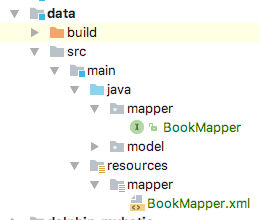
\includegraphics[scale=0.7]{mapperreourcestructure.png}
	\caption{Mapper XML放置目录结构}
	\label{fig:mapperreourcestructure}
\end{figure}


\paragraph{Parameter 'keys' not found. Available parameters are [list]}

在使用MyBatis时,出现如下错误:

\begin{lstlisting}[language=Java]
org.apache.ibatis.binding.BindingException: Parameter 'studentNameList' not found. Available parameters are [list]
\end{lstlisting}

传递一个 List 实例或者数组作为参数对象传给 MyBatis。当你这么做的时 候,MyBatis 会自动将它包装在一个Map中,用名称在作为键。List 实例将会以“list” 作为键,而数组实例将会以“array”作为键。因为此时传的参数只有一个,而且传入的是一个List集合,所以mybatis会自动封装成Map<"list",keys>。在解析的时候会通过“list”作为Map的key值去寻找。但是在xml中却声明成keys了,所以自然会报错找不到。解决办法就是修改Mapper.xml文件。或者将List封装到Map里面传递。第一种方式以后如果要扩展该方法,增加集合参数的时候,需要修改xml中的内容。

\newpage

\chapter{Scala}

截至2017年,采用Scala编写的主要有Spark、Akka。许多企业非关键性组件也会使用Scala构建,Scala相对于Java的优势在语法更加简洁,采用完成相同功能代码量更少,综合来看Scala生产力相对较高。随着硬件性能不断的提升,性能已经不是主要的考虑因素。

\section{函数(Function)}

Scala有两种变量,val和var。val就不能再赋值了。与之对应的,var可以在它生命周期中被多次赋值。数据转换:

\begin{lstlisting}[language=Scala]
//字符串转整型
val errorCodeId: Int = singleErrorCode.toInt;
//split函数
val dstArray: Array[String] = errorCode.toString.split(',')
\end{lstlisting}


\begin{lstlisting}[language=Scala]
case class User(  
	id: Int,  
	firstName: String,  
	lastName: String,  
	age: Int,  
	gender: Option[String])  
	
	object UserRepository {  
	private val users = Map(1 -> User(1, "John", "Doe", 32, Some("male")),  
		2 -> User(2, "Johanna", "Doe", 30, None))  
		def findById(id: Int): Option[User] = users.get(id)  
		def findAll = users.values  
}  
\end{lstlisting}

\subsection{排序}

对Vector中的元素做倒序排序。

\begin{lstlisting}[language=Scala]
/**
* 对要排序的列做反向排序(reverse)
* 全文索引列必须要置于条件的开始
* 否则无法利用索引
* 行政许可XDR列有全文索引,需要排序在前
*/
val params = pageable.getParams.asScala.toVector.reverse  
\end{lstlisting}

\subsection{集合操作}

Scala集合操作如下:

\begin{lstlisting}[language=Scala]
processResult = errorCode.get.split(',')
		.filter(s => StringUtils.isNoneBlank(s))
		.map(code => etlErrorTypeService.findByIntegerId(code.toInt))
		.filter(_ != null)
		.map(eet => eet.getErrDesc)
		.mkString(";")
\end{lstlisting}

mkString把集合元素转化为字符串,可以添加分隔符,前缀,后缀。

\chapter{Python}

Python是FLOSS(自由/开放源码软件)之一。你可以自由地发布这个软件的拷贝、阅读它的源代码、对它做改动、把它的一部分用于新的自由软件中。Python希望看到一个更加优秀的人创造并经常改进。由于它的开源本质,Python已经被移植在许多平台上(经过改动使它能够工作在不同平台上)。如果你小心地避免使用依赖于系统的特性,那么你的所有Python程序无需修改就可以在下述任何平台上面运行。这些平台包括Linux、Windows、FreeBSD、Macintosh、Solaris、OS/2、Amiga、AROS、AS/400、BeOS、OS/390、z/OS、Palm OS、QNX、VMS、Psion、Acom RISC OS、VxWorks、PlayStation、Sharp Zaurus、Windows CE甚至还有PocketPC、Symbian以及Google基于linux开发的Android平台!

\subsection{基础}

查看Python已经安装了哪些模块,可以直接在Python环境中输入help('modules')命令。在Pycharm中设置Python路径在Preference->Project Interpreter中。

\begin{lstlisting}[language=Bash]
# 安装MySQL
sudo apt-get install mysql-server -y
# 安装pip
sudo apt-get install python-pip python-dev build-essential
# 安装MySQL驱动
sudo pip install mysql-python
# 安装beautifulsoup4
sudo pip install beautifulsoup4
# openpyxl来处理xml文件
sudo pip install openpyxl
# 安装Redis支持模块
sudo pip install redis
\end{lstlisting}

在Mac OS X上,提示No Module named requests,使用pip安装requests模块也无法解决,输入如下命令此问题消失:

\begin{lstlisting}[language=Bash]
sudo easy_install -U requests
\end{lstlisting}

pip 改善了不少 easy\_install 的缺點,如此说來 pip 應該是略勝一籌,不過它還不能完全取代對方,因为目前有很多套件還是得用 easy\_install 安裝。easy\_insall的作用和perl中的cpan,ruby中的gem类似,都提供了在线一键安装模块的傻瓜方便方式,而pip是easy\_install的改进版,提供更好的提示信息,删除package等功能。老版本的python中只有easy\_install,没有pip。

\subsection{Beautiful Soup}

Beautiful Soup 是用Python写的一个HTML/XML的解析器,它可以很好的处理不规范标记并生成剖析树(parse tree)。 它提供简单又常用的导航(navigating),搜索以及修改剖析树的操作。Beautiful Soup提供一些简单的、python式的函数用来处理导航、搜索、修改分析树等功能。它是一个工具箱,通过解析文档为用户提供需要抓取的数据,因为简单,所以不需要多少代码就可以写出一个完整的应用程序。如下代码片段展示爬取豆瓣书籍详情页的书籍信息:

\begin{lstlisting}[language=Bash]
def get_single_book_detail_info(url):
try:
req = urllib2.Request(url, headers=hds[np.random.randint(0, len(hds))])
source_code = urllib2.urlopen(req).read()
plain_text = str(source_code)
except (urllib2.HTTPError, urllib2.URLError), e:
print e
soup = BeautifulSoup(plain_text)
list_soup = soup.find('div', {'id': 'info'}).findAll('span')
return list_soup
\end{lstlisting}

find方法直接返回结果,findAll方法返回符合条件的结果。Python在使用前,可以不需要初始化变量,在外层可以直接使用内层函数的变量。

\subsection{爬取豆瓣书籍}

向数据库中保存数据:

\begin{lstlisting}[language=Python]
def save_to_mysql():
	try:
		conn = MySQLdb.connect(host='localhost', user='root', passwd='123456', port=3306)
		cur = conn.cursor()
		conn.select_db('dolphin')
		value = ['hi rollen']
		cur.execute('insert into book(name) values(%s)', value)
		conn.commit()
		cur.close()
		conn.close()
	
	except MySQLdb.Error, e:
		print "Mysql Error %d: %s" % (e.args[0], e.args[1])
\end{lstlisting}

在根据标签爬取的书籍列表中,信息不够全面,比如ISBN号码就没有。所以需要爬到每本书籍的详情页面。

\subsection{抓取技巧}

\paragraph{防止IP被封}在爬取豆瓣的页面时,如果一分钟请求超过一定次数(一说40次),豆瓣会将请求的IP加入黑名单。所以一是爬取的频率不要太高,而是可以使用代理来爬取。服务端对IP访问对阈值也有限制,因为按照正常情况下,一个用户不会大批量对请求一个网站的,所以超过了规定的请求次数也会触发封锁。还可以让请求不那么有规律,让服务器无法通过请求的频率判断是机器还是人类,一般人类访问请求的频率是不固定的。

\paragraph{模仿浏览器}有些网站会检查你是不是真的浏览器访问,还是机器自动访问的。这种情况,加上User-Agent,表明你是浏览器访问即可。有时还会检查是否带Referer信息还会检查你的Referer是否合法,一般再加上Referer。在此次抓取的过程中,模仿浏览器:

\begin{lstlisting}[language=Python]
# Some User Agents
headers = [{'User-Agent': 'Mozilla/5.0 (Windows; U; Windows NT 6.1; en-US; rv:1.9.1.6) Gecko/20091201 Firefox/3.5.6'}, \
{
'User-Agent': 'Mozilla/5.0 (Windows NT 6.2) AppleWebKit/535.11 (KHTML, like Gecko) Chrome/17.0.963.12 Safari/535.11'}, \
{'User-Agent': 'Mozilla/5.0 (compatible; MSIE 10.0; Windows NT 6.2; Trident/6.0)'}]
\end{lstlisting}

在HTTP请求头中,添加浏览器相关标识,让服务器认定为来自浏览器的请求。

\paragraph{避免重复抓取}豆瓣采用Restful风格来设计的API,最后的值就相当于每本书籍的唯一标识,在数据库中预先生成所有的ID集合,每抓取了一个ID的数据,都会更新ID的状态,表示此数据已经抓取。这样的方式来确保每本书籍只被抓取一次。

\paragraph{海量数据}

\subsection{读取Properties文件}

在项目中持续集成的Python部署脚本中,需要读取Java的Properties文件,读取的方法如下:

\begin{lstlisting}[language=Python]
def getVersion():
	#
	#动态从版本配置文件中读取当前最新版本号
	#
	file_path = VERSION_CONFIG_PATH
	props = parse(file_path)   #读取文件
	print('version:'+props.get('VERSION'))
	#根据key读取value
	return props.get('VERSION')            

def parse(file_name):
	return Properties(file_name)
\end{lstlisting}

Propertise类的代码如下:

\begin{lstlisting}[language=Python]
import re
import os
import tempfile

class Properties:

def __init__(self, file_name):
	self.file_name = file_name
	self.properties = {}
	try:
		fopen = open(self.file_name, 'r')
		for line in fopen:
		line = line.strip()
		if line.find('=') > 0 and not line.startswith('#'):
		strs = line.split('=')
		self.properties[strs[0].strip()] = strs[1].strip()
	except Exception, e:
		raise e
	else:
		fopen.close()

def has_key(self, key):
	return key in self.properties

def get(self, key, default_value=''):
	if key in self.properties:
		return self.properties[key]
	return default_value
\end{lstlisting}


\subsection{sh: mysql\_config: command not found解决办法}

首先需要安装MySQL,安装完成后,打开终端,输入下方语句修改环境变量:

\begin{lstlisting}[language=Bash]
# 安装python-devel
sudo dnf install python-devel -y
# 解决fatal error: Python.h: No such file or directory
sudo dnf install python-devel --allowerasing
PATH="$PATH":/usr/local/mysql/bin
\end{lstlisting}

设置完成之后,输入如下语句安装MySQL Python:

\begin{lstlisting}[language=Bash]
sudo pip install mysql-python
\end{lstlisting}

\chapter{前端(Front End)}

\section{React}

只有动画或视频达到60fps,人眼才不会感觉卡顿。

\subsection{组件生命周期(Life Cycle)}

页面的交互流程,页面加载或者用户操作界面,调用相关函数通过Ajax从服务端获取数据,触发dispatch,将action传递给reducer更改state(要赋给propss的值都存在state中),然后再将state的新的值赋给props,重新渲染页面。connect中的函数当state改变时都会被执行,可以理解成subscribe函数或者监听函数。

\subsection{第一个React}

在Web开发中,我们总需要将变化的数据实时反应到UI上,这时就需要对DOM进行操作。而复杂或频繁的DOM操作通常是性能瓶颈产生的原因(如何进行高性能的复杂DOM操作通常是衡量一个前端开发人员技能的重要指标)。React为此引入了虚拟DOM(Virtual DOM)的机制:在浏览器端用Javascript实现了一套DOM API。基于React进行开发时所有的DOM构造都是通过虚拟DOM进行,每当数据变化时,React都会重新构建整个DOM树,然后React将当前整个DOM树和上一次的DOM树进行对比,得到DOM结构的区别,然后仅仅将需要变化的部分进行实际的浏览器DOM更新。如下定义一个最简单的React示例,首先写基本的一个程序入口的组件:

\begin{lstlisting}[language=Javascript]
import React from 'react';
import ReactDOM from 'react-dom';

ReactDOM.render(
	<div>Hello World!</div>,
	document.getElementById('root')
);
\end{lstlisting}

随后定义一个默认的HTML文件:

\begin{lstlisting}[language=HTML]
<body>
	<!-- 容器 -->
	<div id="root"></div>
	<!-- 引入编译好的js文件 -->
	<script type="text/javascript" src="./bundle.js"></script>
</body>
\end{lstlisting}

\subsection{React数据的流转过程}

通过Axios向服务端发送HTTP请求,获取到服务端返回端Json数据后,触发对应Type的dispatch(serviceCommon.js)去更新state。当 state 变化,或者 ownProps 变化的时候,mapStateToProps(connect方法的第一个参数)都会被调用,计算出一个新的 stateProps,(在与 ownProps merge 后)更新给对应的组件。


\subsection{规范(Specification)}

React模块使用.jsx扩展名,如BookMain.jsx。对于JSX属性值总是使用双引号("), 其他均使用单引号。为什么? JSX属性 不能包括转译的引号, 因此在双引号里包括像 "don't" 的属性值更容易输入。HTML属性也是用双引号,所以JSX属性也遵循同样的语法。

\subsection{Router}

Web 服务并不会解析 hash,也就是说 \# 后的内容 Web 服务都会自动忽略,但是 JavaScript 是可以通过 window.location.hash 读取到的,读取到路径加以解析之后就可以响应不同路径的逻辑处理。history 是 HTML5 才有的新 API,可以用来操作浏览器的 session history (会话历史)。在HTML5的history API出现之前,前端的路由都是通过 hash 来实现的,hash 能兼容低版本的浏览器。React Router的设计思想来源于Ember的路由,如果原来有用过Ember的路由,那么应该对React Router不会陌生。React Router 4.0(以下简称 RR4) 已经正式发布,它遵循react的设计理念,即万物皆组件。所以 RR4 只是一堆提供了导航功能的组件(还有若干对象和方法),具有声明式(引入即用),可组合性的特点。添加一个Router组件如下:

\begin{lstlisting}[language=Javascript]
import React from "react";
import {BrowserRouter, Route} from 'react-router-dom'

const User = ({match}) => {
	return <h1>Hello {match.params.username}!</h1>
}

const routes = (
	<BrowserRouter>
		<Route path="/user/:username" component={User}/>
	</BrowserRouter>
);

export default routes;
\end{lstlisting}

<BrowserRouter>是一个使用了HTML5 history API的高阶路由组件,保证你的UI界面和URL保持同步。使用HTML5历史记录API(pushState,replaceState和popstate事件)的<Router>来保持UI与URL的同步。<Route> 也许是RR4中最重要的组件了。它最基本的职责就是当页面的访问地址与 Route 上的 path 匹配时,就渲染出对应的 UI 界面。<Route> 自带三个render method和三个props,props 分别是:match、location、history。所有的render method 无一例外都将被传入这些props。访问效果如图\ref{fig:firstroute}所示:

\begin{figure}[htbp]
	\centering
	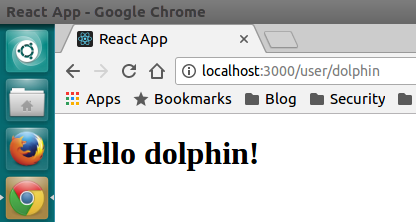
\includegraphics[scale=0.6]{firstroute.png}
	\caption{React Route效果}
	\label{fig:firstroute}
\end{figure}

\paragraph{传入初始值}

项目中需要判断页面是否初次进入,根据是否第一次进入页面还是返回时进入的页面进行不同的逻辑操作,在链接到项目对应模块的地方增加初始参数:

\begin{lstlisting}[language=Javascript]
<Link to={'/profile/redblackLog?operation=init'}>红黑名单访问记录</Link>
\end{lstlisting}

在页面中判断是否第一次进入:

\begin{lstlisting}[language=Javascript]
if (this.props.location.query.operation === "init") {
	//第一次进入页面
}
\end{lstlisting}

\subsection{Provider}

Provider方法会在react组件外边包一层名为provider的组件,使其所有子组件共享store提供的方法。connect方法生成容器组件以后,需要让容器组件拿到state对象,才能生成 UI 组件的参数。一种解决方法是将state对象作为参数,传入容器组件。但是,这样做比较麻烦,尤其是容器组件可能在很深的层级,一级级将state传下去就很麻烦。React-Redux 提供Provider组件,可以让容器组件拿到state。

\begin{lstlisting}[language=Javascript]
ReactDOM.render(
	<Provider store={store}>{routes}</Provider>,
	document.getElementById('root')
);
\end{lstlisting}

Provider在根组件外面包了一层,这样一来,App的所有子组件就默认都可以拿到state了。同理store只需要在最顶层导入一次,否则在下级的每一个组件都需要导入store,非常不利于组件复用,每个组件都导入显然不够优雅,它的原理是React组件的context属性。

\subsection{Connect}

React-Redux 提供connect方法,用于从 UI 组件生成容器组件。connect的意思,就是将这两种组件连起来。

\begin{lstlisting}[language=Javascript]
connect(mapStateToProps, mapDispatchToProps, mergeProps)(MyComponent)
\end{lstlisting}

项目中connect定义如下:

\begin{lstlisting}[language=Javascript]
/**
* mapStateToProps:这个函数的作用是确定哪些 Redux 全局的 state 是我们组件想要通过 props 获取
*/
const mapStateToProps = (state) => {
	return {
		book: state.book
	}
}

/**
* mapDispatchToProps:这个方法的作用是确定 哪些action创建函数是我们想要通过props获取
*/
const mapDispatchToProps = (dispatch) =>{
	return{
		bookService: bindActionCreators(bookService, dispatch)
	}
}

connect(mapStateToProps, mapDispatchToProps)
	class BookContainer extends Component {
	render() {
		return React.cloneElement(this.props.children, {...this.props});
	}
}
\end{lstlisting}

\subsection{Actions}

Action向store派发指令,action 函数会返回一个带有 type 属性的 Javascript Plain Object,store将会根据不同的action.type来执行相应的方法。

\subsection{Store}

为什么要使用store?如果不使用store,那么各个组件的数据必须由各个组件来维护,这种情况会出现一些问题,第一就是组件之间的数据可能会有重复,比如一个组件父组件统计子组件的数据,父组件需要存储子组件的数据,子组件也会存储自己的数据,数据重复又会带来问题,数据之间的维护需要大量的工作(子组件数据更新后父组件的数据也要更新),多份数据的情况下非常容易造成数据不一致。这也就是为什么要使用store,而且整个应用中只能有一个store的原因\footnote{参考《深入浅出React和Redux》2.5小节}。store是应用的状态管理中心,保存着是应用的状态(state),当收到状态的更新时,会触发视觉组件进行更新。Provider是react-redux提供的组件,它的作用是把store和视图绑定在了一起,如下语句创建一个简单的store。

\begin{lstlisting}[language=Javascript]
import {createStore} from 'redux';
//创建store
const store = createStore(reducer, 1);
\end{lstlisting}

第一个参数为reducer,第二个参数是初始化的状态(initialState),这里为1。

\subsection{Dispatcher}

接收action,并且向注册的回调函数广播payloads。Facebook还提供了Dispatcher的开源库。你可以将Dispatcher认为是一种全局pub/sub系统的事件处理器,用于向所注册的回调函数广播payloads。通常情况下,如果你使用Flux架构,你可以借助于Facebook提供的这个Dispatcher实现,并且可以借助NodeJS中的EventEmitter模块来配置事件系统, 从而帮助管理应用程序的状态。Store中包括了注册给Dispatcher的回调函数。actionCreator还有很简洁的用法:对actionCreator做dispatch级别的封装,这个过程我们可以使用 redux 提供的 bindActionCreators 函数自动完成。然后就可以直接调用action,而不需要使用dispatch方法去调用actionCreator。dispatch调用如下代码片段所示。

\begin{lstlisting}[language=Javascript]
store.dispatch({
	type: "ARTICLE_PAGE",
	payload: 10
});
\end{lstlisting}

dispatch的参数是一个Action。如下代码片段定义一个Action:

\begin{lstlisting}[language=Javascript]
const action = {
	type: "ARTICLE_PAGE",
	payload: 10
};
\end{lstlisting}

其中的type属性是必须的,表示 Action 的名称。上面代码中,Action 的名称是ARTICLE\_PAGE,它携带的信息是数字10。

\paragraph{redux-thunk}

解决了dispatch不好获取的问题。Redux官网说,action就是Plain JavaScript Object。Thunk允许action creator返回一个函数,而且这个函数第一个参数是dispatch。例如:

\begin{lstlisting}[language=Javascript]
export function findPage(params) {
	return dispatch =>
		requestJSON(
			dispatch,
			{method: 'get', url: '/pubapi/article/page', params: {...params}},
			{type: articleTYPE.ARTICLE_PAGE},
			{type: articleTYPE.ARTICLE_PAGE_ERROR, message: '获取文章列表失败'});
}
\end{lstlisting}

在异步Action时也需要使用thunder中间件。以上代码片段就是一个更好的例子,以上代码表示向服务器发送一个请求获取文章列表,但是这里返回的是一个函数,而不是一个对象,redux-thunder的工作就是检查action对象是不是函数,如果不是函数就放行,让其执行完整的action-reducer-view生命周期。如果发现对象是函数,就执行这个函数,并把Store的dispatch函数和getState函数作为参数传递到函数中去,处理过程到此为止,不会让异步对象再派发到reducer函数。异步调用的API再根据合适的时机派发Action,触发界面Render\footnote{参考《深入浅出React和Redux》7.2.2节}。

\subsection{Reducer}

Store收到Action以后,必须给出一个新的State,这样View才会发生变化。这种State的计算过程就叫做Reducer。
Reducer是一个函数,它接受Action和当前State作为参数,返回一个新的State。如下语句创建一个简单的Reducer:

\begin{lstlisting}[language=Javascript]
const reducer = (state, action) => {
	switch (action.type) {
		case "ADD":
			state = state + action.payload;
			break;
		case "SUBTRACT":
			break;
	}
	return state;
};
\end{lstlisting}

\subsection{state}

State (也称为 state tree) 是一个宽泛的概念,但是在 Redux API 中,通常是指一个唯一的 state 值,由 store 管理且由 getState() 方法获得。它表示了 Redux 应用的全部状态,通常为一个多层嵌套的对象。约定俗成,顶层 state 或为一个对象,或像 Map 那样的键-值集合,也可以是任意的数据类型。然而你应尽可能确保 state 可以被序列化,而且不要把什么数据都放进去,导致无法轻松地把 state 转换成 JSON\footnote{来源:\url{http://cn.redux.js.org/docs/Glossary.html}}。state是React中组件的一个对象.React把用户界面当做是状态机,想象它有不同的状态然后渲染这些状态,可以轻松让用户界面与数据保持一致.React中,更新组件的state,会导致重新渲染用户界面(不要操作DOM).

\begin{lstlisting}[language=Javascript]
//会重新渲染页面
this.setState({query: query});
/*
 * 不会重新渲染页面
 * 调用this.forceUpdate()手动强制重新渲染页面
 */
this.setState.query = query;
this.forceUpdate();
\end{lstlisting}

一般情况下应该用setState来设置state值,不应该对state直接赋值\footnote{\url{参考:https://reactjs.org/docs/state-and-lifecycle.html}}(It is better to use this.setState because it is init native check-state mecanizm of React engine which is better then force update.If you just update any param of this.state directly without setState react render mecanizm will not know that some params of state is updated.),对state直接赋值可以在构造方法中(The only place where you can assign this.state is the constructor)。还有一点需要注意的是setState方法是异步的,可以使用回调(Callback)函数来获取最终结果:

\begin{lstlisting}[language=Javascript]
//使用回调函数获取设置的值
this.setState({data: data}, function(){
	console.log(this.state.data);
}.bind(this));
\end{lstlisting}

\paragraph{初始化state}

有2种方法来初始化应用的state,一种是在createStore方法中的第二个可选参数preloadState。也可以在reducer中为undefined的state参数指定默认初始值。state的结构如图\ref{fig:statedemo}所示。

\begin{figure}[htbp]
	\centering
	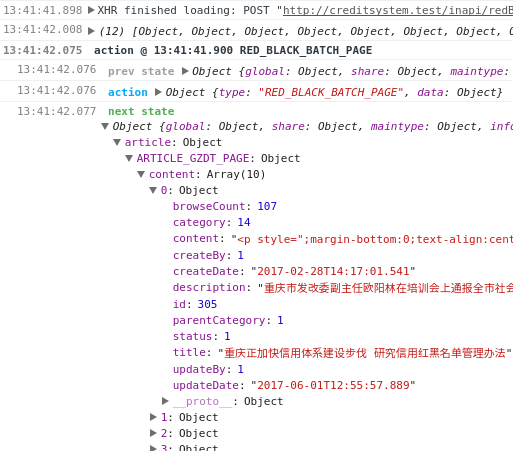
\includegraphics[scale=0.6]{statedemo.png}
	\caption{State状态示例}
	\label{fig:statedemo}
\end{figure}



\paragraph{redux logger}

Redux Logger是一个中间件,它会打印出当前应用的state变化,配置如下代码所示。

\begin{lstlisting}[language=Javascript]
/**
* ES6 with npm, you can write import React from 'react'. 
* ES5 with npm, you can write var React = require('react').
*/
import {createLogger} from 'redux-logger';

if (process.env.NODE_ENV === 'development') {
	const logger = createLogger({
	stateTransformer: (state) => {
		let newState = {};
		for (let i of Object.keys(state)) {
			if (Iterable.isIterable(state[i])) {
					newState[i] = state[i].toJS();
				} else {
					newState[i] = state[i];
				}
			}
			return newState;
		}
	});
	middleware.push(logger);
}
\end{lstlisting}

打印出action的效果如图\ref{fig:reduxloggerexample}所示。

\begin{figure}[htbp]
	\centering
	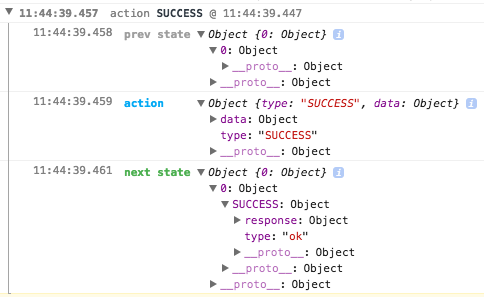
\includegraphics[scale=0.6]{reduxloggerexample.png}
	\caption{Redux Logger打印效果}
	\label{fig:reduxloggerexample}
\end{figure}

从图中看出,state的状态已经改变。说明是state改变后的某些动作还未触发。

\subsection{Props}

当你用React Redux的connect进行封装的时候,connect方法会把dispatch放到props中。

\paragraph{React Router父子Props传递}

在React中需要将bookService由父组件中传递到子组件中,写法如下:

\begin{lstlisting}[language=Javascript]
const routes = (
<BrowserRouter>
	<BookContainer>
		<switch>
			<Route path="/book/:id" render={() => <Book bookService={bookService}/>}/>
		</switch>
	</BookContainer>
</BrowserRouter>
);
\end{lstlisting}

其中Book处于内层,负责渲染界面,所以叫做展示组件(Presentational Container)。BookContainer与Book组件属于父子组件的关系,BookContainer负责和Redux Store打交道,处于外层,称作容器组件(Container Component)。容器组件的定义如下:

\begin{lstlisting}[language=Javascript]
/**
* 容器组件,负责与Redux Store打交道
* 通过props把状态传递给内层组件
*/
class BookContainer extends Component {
	render() {
		return React.cloneElement(this.props.children, {...this.props});
	}
}
\end{lstlisting}

在浏览器中,切换到相应组件上,可以看到对应的属性,如图\ref{fig:bookserviceprops}所示。

\begin{figure}[htbp]
	\centering
	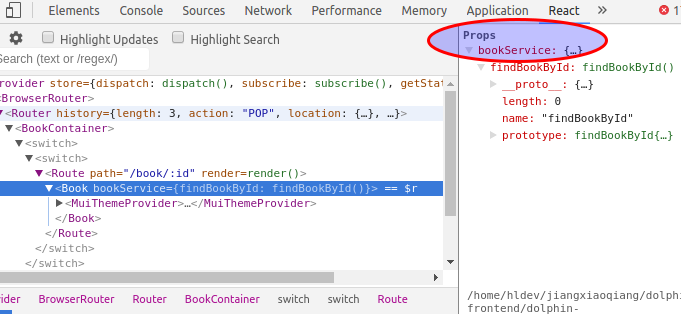
\includegraphics[scale=0.5]{bookserviceprops.png}
	\caption{React 组件Props传递}
	\label{fig:bookserviceprops}
\end{figure}

还可以传递函数,例如有时候在子组件上操作后需要更新父组件的界面,可以将更新方法通过Props传递给子组件,子组件直接调用函数进行更新即可。

\begin{lstlisting}[language=Javascript]
/**
* refreshFetch是父组件定义的函数
*/
return <FeedbackPanel query={query}
						refreshFetch={this.refreshFetch}
						creditFormTable={creditFormTable}
						key={i}/>
\end{lstlisting}

\subsection{Reducers}

Redux有且只有一个State状态树,为了避免这个状态树变得越来越复杂,Redux通过 Reducers来负责管理整个应用的State树,而Reducers可以被分成一个个Reducer。


\paragraph{onEnter}

Route 的 onEnter 钩子将用于在渲染对象的组件前做拦截操作,比如验证权限。单页应用路由的权限控制的基本思路是:监听路由的改变,每当路由将要发生改变,我们就使用一个中间服务(该服务介于上一级路由和将要到达路由之间启动),来判断我们是否有进入这个路由的权限,有的话直接进入,没有的话就redirect。在React中,为某个路由进行权限监听的方式是:

\begin{lstlisting}[language=HTML]
<Route path="page" component={Page} onEnter={requireCredentials}/>
\end{lstlisting}

该onEnter属性对应连着一个具有判断权限的中间服务。

\subsection{Immutable}

JavaScript 中的对象一般是可变的(Mutable),因为使用了引用赋值,新的对象简单的引用了原始对象,改变新的对象将影响到原始对象。如 foo={a: 1}; bar=foo; bar.a=2 你会发现此时 foo.a 也被改成了 2。虽然这样做可以节约内存,但当应用复杂后,这就造成了非常大的隐患,Mutable 带来的优点变得得不偿失。为了解决这个问题,一般的做法是使用 shallowCopy(浅拷贝)或 deepCopy(深拷贝)来避免被修改,但这样做造成了 CPU 和内存的浪费。Immutable 可以很好地解决这些问题。

\paragraph{IMMUTABLE DATA}

Immutable Data 就是一旦创建,就不能再被更改的数据。对 Immutable 对象的任何修改或添加删除操作都会返回一个新的 Immutable 对象。Immutable 实现的原理是 Persistent Data Structure(持久化数据结构),也就是使用旧数据创建新数据时,要保证旧数据同时可用且不变。同时为了避免 deepCopy 把所有节点都复制一遍带来的性能损耗,Immutable 使用了 Structural Sharing(结构共享),即如果对象树中一个节点发生变化,只修改这个节点和受它影响的父节点,其它节点则进行共享。

\subsection{前端Mock}

有的时候前端没必要等待后端接口写好,可以直接Mock接口的返回数据。这里使用json-server\footnote{\url{https://github.com/typicode/json-server}}来实现。

\section{MobX}

\subsection{简介}

mobx 是一个库 (library),不是一个框架 (framework)。可以和React组合使用,MobX is a battle tested library that makes state management simple and scalable by transparently applying functional reactive programming (TFRP). React and MobX together are a powerful combination. redux 管理的是 (STORE -> VIEW -> ACTION) 的整个闭环,而 mobx 只关心 STORE -> VIEW 的部分。

\section{gulp}

Gulp基于Node.js的前端构建工具,通过Gulp的插件可以实现前端代码的编译(sass、less)、压缩、测试;图片的压缩;浏览器自动刷新。比起Grunt不仅配置简单而且更容易阅读和维护。gulpjs是一个前端构建工具,与gruntjs相比,gulpjs无需写一大堆繁杂的配置参数,API也非常简单,学习起来很容易,而且gulpjs使用的是nodejs中stream来读取和操作数据,其速度更快。使用 browserify 进行打包, gulp 进行任务构建。由于使用了 ES2015 和 JSX 语法,因此使用 Babel 进行转换。

\begin{itemize}
	\item{压缩js代码(gulp-uglify)}
	\item{压缩图片(gulp-imagemin)}
\end{itemize}

\subsection{压缩图片}

首先,定义一个压缩图片的任务:

\begin{lstlisting}[language=JavaScript]
gulp.task('images', function() {
	return gulp.src('src/images/**/*')
			.pipe(imagemin({ optimizationLevel: 3, progressive: true, interlaced: true }))
			.pipe(gulp.dest('dist/assets/img'))
			.pipe(notify({ message: 'Images task complete' }));
});
\end{lstlisting}

定义一个名称为images的任务,这个任务使用imagemin插件把所有在src/images/目录以及其子目录下的所有图片(文件)进行压缩,可以进一步优化,利用缓存保存已经压缩过的图片。在终端中运行如下命令执行此任务。

\begin{lstlisting}[language=Bash]
gulp images
\end{lstlisting}

\subsection{清除文件}

在再次生成文件前,最好先清除之前生成的文件:

\begin{lstlisting}[language=JavaScript]
gulp.task('clean', function(cb) {
	del(['dist/assets/css', 'dist/assets/js', 'dist/assets/img'], cb)
});
\end{lstlisting}

在这里没有必要使用Gulp插件了,可以使用NPM提供的插件。用一个回调函数(cb)确保在退出前完成任务。

\subsection{设置默认任务}

\begin{lstlisting}[language=JavaScript]
gulp.task('default', ['clean'], function() {
	gulp.start('styles', 'scripts', 'images');
});
\end{lstlisting}

clean任务执行完成了才会去运行其他的任务,在gulp.start()里的任务执行的顺序是不确定的,所以将要在它们之前执行的任务写在数组里面。

\section{webpack}

使用install --save时,将默认在package.json中添加小尖尖\^而不是小波浪\~作为依赖版本的前缀。

\section{Library}

\subsection{lodash}

lodash是一个具有一致接口、模块化、高性能等特性的 JavaScript 工具库。

\paragraph{去除重复数据}

去除重复数据:

\begin{lstlisting}[language=JavaScript]
import lodashUniqBy from "lodash/uniqBy";
const uniqOrgList = lodashUniqBy(orgList, 'dfName');
\end{lstlisting}

\paragraph{分组}

将数组中的元素按照新的方式返回。

\begin{lstlisting}[language=JavaScript]
/**
* 将部门按照10个1组组成一个新数组返回
*/
return lodashChunk(dfbmList, 10).map((dfbms, rowNo) => {
		const items = this.renderItems(groups, dfbms);
		return (
		});
\end{lstlisting}

\paragraph{排序}

数组使用lodash排序如下代码所示:

\begin{lstlisting}[language=JavaScript]
import lodash from 'lodash';
/**
* 按照登录数量排序
*/
const top10Datasource = lodash.sortBy(this.loginCount(), function (item) {
	item.count;
});
\end{lstlisting}

\subsection{Axios}

axios是一个基于Promise用于浏览器和nodejs的HTTP客户端。ES6 原生提供了 Promise 对象。所谓 Promise,就是一个对象,用来传递异步操作的消息。它代表了某个未来才会知道结果的事件(通常是一个异步操作),并且这个事件提供统一的 API,可供进一步处理。

Promise 对象有以下两个特点。

(1)对象的状态不受外界影响。Promise 对象代表一个异步操作,有三种状态:Pending(进行中)、Resolved(已完成,又称 Fulfilled)和 Rejected(已失败)。只有异步操作的结果,可以决定当前是哪一种状态,任何其他操作都无法改变这个状态。这也是 Promise 这个名字的由来,它的英语意思就是「承诺」,表示其他手段无法改变。

(2)一旦状态改变,就不会再变,任何时候都可以得到这个结果。Promise 对象的状态改变,只有两种可能:从 Pending 变为 Resolved 和从 Pending 变为 Rejected。只要这两种情况发生,状态就凝固了,不会再变了,会一直保持这个结果。就算改变已经发生了,你再对 Promise 对象添加回调函数,也会立即得到这个结果。这与事件(Event)完全不同,事件的特点是,如果你错过了它,再去监听,是得不到结果的。

有了 Promise 对象,就可以将异步操作以同步操作的流程表达出来,避免了层层嵌套的回调函数。此外,Promise 对象提供统一的接口,使得控制异步操作更加容易。

Promise 也有一些缺点。首先,无法取消 Promise,一旦新建它就会立即执行,无法中途取消。其次,如果不设置回调函数,Promise 内部抛出的错误,不会反应到外部。第三,当处于 Pending 状态时,无法得知目前进展到哪一个阶段(刚刚开始还是即将完成)。

\subsection{Axios请求}

一个简单的Axios请求示例如下:

\begin{lstlisting}[language=JavaScript]
import axios from 'axios';

export function request() {
	return axios({
			method: 'get', url: 'http://localhost:8011/api/book/111'
		}).then(
		response => {
			console.log(response)
		}
		).catch(
			error => {
			console.error(error);
		}
	);
}
\end{lstlisting}


这里需要解决跨域问题,通过Node或Nginx等做Proxy,或者在服务器端配置CORS。

\subsection{Axios拦截响应}

拦截响应可以对服务端抛出的错误做统一的handle:

\begin{lstlisting}[language=JavaScript]
/**
* axios响应拦截器
*/
axios.interceptors.response.use(
		response =>{
		return response;
	},
	error => {
		if(error.response){
			switch (error.response.status){
				case 401:
					responseError401PreHandle(error.response.data);
					break;
				case 403:
			}
		}
	}
);
\end{lstlisting}

\subsection{Promise}

为了降低异步编程的复杂性,开发人员一直寻找简便的方法来处理异步操作。其中一种处理模式称为promise,它代表了一种可能会长时间运行而且不一定必须完整的操作的结果。这种模式不会阻塞和等待长时间的操作完成,而是返回一个代表了承诺的(promised)结果的对象。promise模式通常会实现一种称为then的方法,用来注册状态变化时对应的回调函数。promise模式在任何时刻都处于以下三种状态之一:未完成(unfulfilled)、已完成(resolved)和拒绝(rejected)。Promise.reject返回了一个拒绝状态的Promise对象. 对于这样的Promise对象, 如果其后续then | catch中都没有声明onRejected回调, 它将会抛出一个 “Uncaught (in promise) …”的错误. Promise之间泾渭分明, 内部Promise抛出的任何错误,外部Promise对象都无法感知并捕获. 同时, 由于promise是异步的, try catch语句也无法捕获其错误.因此养成良好习惯, promise记得写上catch.

\section{Cookie}

The browser is expected to support 20 cookies for each Web server, 300 cookies total, and may limit cookie size to 4 KB each.在Chrome中查看Cookie可以直接在Console中输入:

\begin{lstlisting}[language=Bash]
document.cookie
\end{lstlisting}

服务器端像客户端发送Cookie是通过HTTP响应报文实现的,在Set-Cookie中设置需要像客户端发送的cookie,cookie格式如下:

\begin{lstlisting}
Set-Cookie: “name=value;domain=.domain.com;path=/;expires=Sat, 11 Jun 2016 11:29:42 GMT;HttpOnly;secure”
\end{lstlisting}

其中name=value是必选项,其它都是可选项。如果在Cookie中设置了"HttpOnly"属性,那么通过程序(JS脚本、Applet等)将无法读取到Cookie信息,这样能有效的防止XSS攻击。当secure设置为true时,表示创建的 Cookie 会被以安全的形式向服务器传输,也就是只能在 HTTPS 连接中被浏览器传递到服务器端进行会话验证,如果是 HTTP 连接则不会传递该信息,所以不会被盗取到Cookie 的具体内容。Cookie的主要构成如下:

\begin{lstlisting}
name:一个唯一确定的cookie名称。通常来讲cookie的名称是不区分大小写的。
value:存储在cookie中的字符串值。最好为cookie的name和value进行url编码
domain:cookie对于哪个域是有效的。所有向该域发送的请求中都会包含这个cookie信息。这个值可以包含子域(如:yq.aliyun.com),也可以不包含它(如:.aliyun.com,则对于aliyun.com的所有子域都有效).
path: 表示这个cookie影响到的路径,浏览器跟会根据这项配置,像指定域中匹配的路径发送cookie。
expires:失效时间,表示cookie何时应该被删除的时间戳(也就是,何时应该停止向服务器发送这个cookie)。如果不设置这个时间戳,浏览器会在页面关闭时即将删除所有cookie;不过也可以自己设置删除时间。这个值是GMT时间格式,如果客户端和服务器端时间不一致,使用expires就会存在偏差。
max-age: 与expires作用相同,用来告诉浏览器此cookie多久过期(单位是秒),而不是一个固定的时间点。正常情况下,max-age的优先级高于expires。
HttpOnly: 告知浏览器不允许通过脚本document.cookie去更改这个值,同样这个值在document.cookie中也不可见。但在http请求张仍然会携带这个cookie。注意这个值虽然在脚本中不可获取,但仍然在浏览器安装目录中以文件形式存在。这项设置通常在服务器端设置。
secure: 安全标志,指定后,只有在使用SSL链接时候才能发送到服务器,如果是http链接则不会传递该信息。就算设置了secure 属性也并不代表他人不能看到你机器本地保存的 cookie 信息,所以不要把重要信息放cookie就对了
\end{lstlisting}

\paragraph{Max Age}查看Cookie类的setMaxAge(int expiry)方法说明:这个类用于给Cookie设置最大的年龄,以秒为单位。expiry - an integer specifying the maximum age of the cookie in seconds; if negative, means the cookie is not stored; if zero, deletes the cookie.如果这个方法的参数给的是正值,表明cookie在超过指定的年龄时间后会消亡。负值意味着cookie不是永久性存储的,在浏览器关闭的时候将会被删除。这个方法的参数如果是零值将会导致cookie被删除。Expire指定了cookie的生存期,默认情况下cookie是暂时存在的,他们存储的值只在浏览器会话期间存在,当用户推出浏览器后这些值也会丢失,如果想让cookie存在一段时间,就要为expires属性设置为未来的一个过期日期。现在已经被max-age属性所取代,max-age用秒来设置cookie的生存期。

\section{Javascript}

\begin{tabular}{cp{8cm}c}
	\hline
	\multirow{1}{*}{快捷键}
	& \multicolumn{1}{c}{说明}  \\
	\hline			
	nbsp & " " \\
	\hline
\end{tabular}


\subsection{prototype}

prototype是用于解决实例对象之间无法共享属性和方法的。

\begin{lstlisting}[language=Javascript]
function Tiger(name){
	this.name = name;
	this.species = "猫科";
}
var tigerA = new Tiger("大虎");
var tigerB = new Tiger("二虎");
tigerA.species="犬科";
console.log(tigerB.species);//猫科
\end{lstlisting}

此处无法做到数据共享,也是极大的资源浪费。其实species共享是符合设计的。使用prototype来实现共享:

\begin{lstlisting}[language=Javascript]
function Tiger(name) {
	this.name = name;
}
Tiger.prototype = {
	species: '犬科'
};
var tigerA = new Tiger("大虎");
var tigerB = new Tiger("二虎");
console.log(tigerA.species);//犬科
console.log(tigerB.species);//犬科
Tiger.prototype.species = '猫科';
console.log(tigerA.species);//猫科
console.log(tigerB.species);//猫科
\end{lstlisting}

注意这里是设置Tiger的prototype而不是Tiger实例的prototype。一个未初始化的变量的值为undefined,一个没有传入实参的形参变量的值为undefined,如果一个函数什么都不返回,则该函数默认返回undefined.所以这里在控制台最后会打印一行undefined。普通对象设置prototype使用如下语句:

\begin{lstlisting}[language=Javascript]
tigerA.__proto__.species = '犬科';
\end{lstlisting}

\subsection{常用函数}

\paragraph{正则匹配定长数字}

采用如下函数验证定长数字:

\begin{lstlisting}[language=Javascript]
isFixedNumber = (rule, value, callback) => {
	if (/^\d{1,6}$/.test(value)) {
		callback();
	} else {
		callback('机构ID只能是6位数字');
	}
}
\end{lstlisting}


\paragraph{下划线命名转驼峰命名}

如下函数将下划线命名的方式转成驼峰命名的方式:

\begin{lstlisting}[language=Javascript]
function camelCase(input) {
		return input.toLowerCase().replace(/_(.)/g, function (match, group1) {
		return group1.toUpperCase();
	});
}
//XDR\_SHXYM转换结果xdrShxym
const camelName =camelCase("XDR_SHXYM");
\end{lstlisting}

数学函数:

\begin{lstlisting}[language=Javascript]
f = Math.round(x / 10000 * Math.pow(10, y)) / Math.pow(10, y);
\end{lstlisting}

Math.pow计算10的y次幂,Math.round计算与round函数最接近的整数。

\begin{lstlisting}[language=HTML]
#默认会执行一次
<button onClick={this.getBookInfo()}>查询</button>
#默认不会执行
<button onClick={() => this.getBookInfo()}>查询</button>
\end{lstlisting}

对象转数组:

\begin{lstlisting}[language=Javascript]
const books = this.props.books;
	let arr = [];
	for(let i in books){
	arr.push(books[i]);
}
\end{lstlisting}

判断值是不是空:

\begin{lstlisting}[language=Javascript]
if (!value || (value + ' ').trim().length === 0) {
	/**
	* 值为空的字段在界面上不显示
	* 如果value是整数,不能使用trim(),所以加字符串手动转换成String类型
	*/
	return;
}

/**
* 如果需要判断字符串为空,直接if判断即可
*/
if(value){
	/**
	* 此种写法等价于if(value===null||value===undefined||value==='')
	*/
}
\end{lstlisting}

\subsection{日期处理}

Moment.js是一个JavaScript日期处理类库,如下代码片段使用moment格式化日期。

\begin{lstlisting}[language=Javascript]
import moment from "moment";

tableDataSource = (logList, orgList) => {
	const content = logList.content || [];
	return content.map((item, idx) => {
		const org = orgList.find(org => org.orgId == item.ORG_ID);
		return {
			...item,
			//格式化日期
			QUERY_DATE: moment(item.QUERY_DATE).format("YYYY-MM-DD hh:mm:ss"),
		};
	})
};
\end{lstlisting}

获取本周的第一天,moment中可以用如下代码实现:

\begin{lstlisting}[language=Javascript]
moment.lang('zh-cn', {
week: {
	dow: 1 // Monday is the first day of the week
}
});
// date now is the first day of the week, (i.e., Monday)
const date = moment().weekday(0); 
\end{lstlisting}

\section{常见问题}

\paragraph{页面卡顿}

一次页面卡顿是由于服务端某一个页面返回了过多的数据6w多。

\paragraph{index.js:83 TypeError: Cannot read property 'get' of undefined}

出現此錯誤的原因是獲取到的參數爲空。

\begin{lstlisting}
TypeError: Cannot read property 'get' of undefined
at Object.getToJS (Utils.js:171)
at Object.getToArray (Utils.js:166)
at CreditDataPeopleMain.render (CreditDataPeopleMain.js:299)
at eval (ReactCompositeComponent.js:796)
at measureLifeCyclePerf (ReactCompositeComponent.js:75)
at ReactCompositeComponentWrapper._renderValidatedComponentWithoutOwnerOrContext (ReactCompositeComponent.js:795)
at ReactCompositeComponentWrapper._renderValidatedComponent (ReactCompositeComponent.js:822)
at ReactCompositeComponentWrapper.performInitialMount (ReactCompositeComponent.js:362)
at ReactCompositeComponentWrapper.mountComponent (ReactCompositeComponent.js:258)
at Object.mountComponent (ReactReconciler.js:46)
\end{lstlisting}

獲取到的空數據如圖\ref{fig:getundefineerror}所示。

\begin{figure}[htbp]
	\centering
	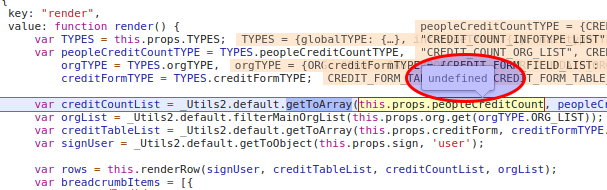
\includegraphics[scale=0.5]{getundefineerror.png}
	\caption{undefined錯誤}
	\label{fig:getundefineerror}
\end{figure}

由于采用的是React,说明获取到的数据没有映射到对象里面。在store.js里面添加对应的缺少的实体即可。在错误处点击进去跟踪到相应的实体值为undefine的,添加到store文件中即可。

\paragraph{Each child in an array or iterator should have a unique "key" prop. Check the render method of `CreditDataPeopleMain`}

提示在數組和可枚舉中需要給定一個唯一的key屬性:

\begin{lstlisting}
Warning: Each child in an array or iterator should have a unique "key" prop. Check the render method of `CreditDataPeopleMain`. See https://fb.me/react-warning-keys for more information.
in a (created by CreditDataPeopleMain)
in CreditDataPeopleMain (created by RouterContext)
in SharingExchangeContainer (created by Connect(SharingExchangeContainer))
in Connect(SharingExchangeContainer) (created by RouterContext)
in div (created by AppContainer)
in div (created by AppContainer)
in div (created by AppContainer)
in AppContainer (created by RouterContext)
in RouterContext (created by Router)
in Router
in Provider
\end{lstlisting}

key屬性幫助react確定項目是否已經更新(Keys help React identify which items have changed, are added, or are removed. Keys should be given to the elements inside the array to give the elements a stable identity)。

\paragraph{Cannot read property 'apply' of undefined}

\paragraph{Module build failed: SyntaxError: Unexpected token ...}

...是ES6中的扩展运算符(Spread Operator),需要将之转化为ES5语法,转换使用babel来完成,presets字段设定转码规则,检查是否安装包:

\begin{lstlisting}[language=Javascript]
"devDependencies": {
	"babel-core": "^6.25.0",
	"babel-loader": "^7.1.0",
	"babel-preset-es2015": "^6.24.1",//ES2015转码规则
	"babel-preset-react": "^6.24.1",
	//ES7不同阶段语法提案的转码规则(共有4个阶段)
	//从stage-0到stage-3
	"babel-preset-stage-0": "6.22.0"
}
\end{lstlisting}

检查Webpack中的配置:

\begin{lstlisting}[language=Javascript]
module: {
	loaders: [{
		test: /\.(jsx|js)?$/,   // 匹配jsx语法规则
		exclude: /node_modules/,   // 排除的模块
		loaders: 'babel-loader',   // loader名
		query: {
			// 将react预置为es5
			presets: ['es2015', 'react','stage-0']
		}
	}]
}
\end{lstlisting}

\paragraph{Store does not have a valid reducer}

提示错误:Store does not have a valid reducer. Make sure the argument passed to combineReducers is an object whose values are reducers.store在index.js文件中引入,在store.js中添加打印语句将reducer对象打印出来,看到实际是有reducer对象的,所以怀疑是reducer的定义有些问题。最后发现原来是require的使用有问题。

\begin{lstlisting}[language=Javascript]
const state = {};
for (const name of nameList) {
	state[name] = require(`./${name}/${name}Reducer`);
}
\end{lstlisting}

这里是用Requre动态加载,但是实际有点问题,暂时还找不到原因。暂时采用如下的写法:


\begin{lstlisting}[language=Javascript]
import bookReducer from './book/bookReducer';
state[0] = bookReducer;
\end{lstlisting}

\clearpage

\part{OS}

\chapter{Linux}\index{Linux}

在使用apt-get时,有时可能会遇到依赖损坏的情况,那么可以执行如下命令,尝试修复依赖:

\begin{lstlisting}[language=Bash]
sudo apt-get -f install 
\end{lstlisting}

f参数表示尝试修正系统依赖损坏处。

\section{Shell}

\subsection{自动部署(Auto Deploy)}

最初使用Shell脚本是将之用于自动化部署应用程序。一般部署程序步骤皆是重复的,编译、构建、打包、拷贝、备份网站、停止旧版网站启动新版Beta网站,Beta网站出现问题时,Rollback到Stable版本,可以使用Shell脚本将重复的操作自动化。将项目在本地打包,打包文件拷贝到目标服务器(一台或多台)上,自动启动应用程序。

\begin{lstlisting}[language=Bash]
#!/usr/bin/env bash

#
# 一键部署后端项目到远程1台或多台服务器
# 发布流程为:编译构建-打包-发布包-拷贝包到指定目录-解压包
# 注:本机需要安装Ansible并与服务器做免密登录
#
# 2017-05-25 增加动态读取版本号,根据版本自动发布程序
#

# 当使用未初始化的变量时,程序自动退出
set -u

# 当任何一行命令执行失败时,自动退出脚本
set -e

# send=`date '+%Y-%m-%d %H:%M:%S'`
CURRENT\_TIME=`date '+%Y%m%d%H%M%S'`

echo "$CURRENT_TIME"

PROGRAM_PATH_INFORMATION_CENTER="/opt/app/backend"
SERVER_IP="192.168.1.101"
LOGIN_USER="root"
LOCAL_PATH="./cc-web-boot/build/libs"

# Read program version number
source version.properties
echo "$VERSION"

PROGRAM_NAME="credit-system-web-boot-$VERSION.jar"
echo "$PROGRAM_NAME"

echo "开始构建..."
# Build project
./gradlew -p cc-web-boot -x test build
./gradlew -p cc-etl-sechedule -x test build

echo "开始拷贝..."
# publish project
scp $LOCAL_PATH/$PROGRAM_NAME $LOGIN_USER@$SERVER_IP:~/app-soft/
scp start.sh $LOGIN_USER@$SERVER_IP:$PROGRAM_PATH_INFORMATION_CENTER
scp version.properies $LOGIN_USER@$SERVER_IP:$PROGRAM_PATH_INFORMATION_CENTER

ansible webservers -m command -a "date"

echo "停止站点..."
ansible webservers -m command -a "chdir=$PROGRAM_PATH_INFORMATION_CENTER bash ./stop.sh"

echo "等待站点停止..."
sleep 10

echo "备份站点..."
# 备份当前站点
ansible webservers -m command -a "mv $PROGRAM_PATH_INFORMATION_CENTER/$PROGRAM_NAME $PROGRAM_PATH_INFORMATION_CENTER/$PROGRAM_NAME-$CURRENT_TIME"

echo "拷贝新文件..."
ansible webservers -a "mv ~/app-soft/$PROGRAM_NAME $PROGRAM_PATH_INFORMATION_CENTER"

echo "启动站点..."
ansible webservers -m shell -a "bash ./start.sh chdir=$PROGRAM_PATH_INFORMATION_CENTER"

echo "部署完成"
\end{lstlisting}

start.sh和stop.sh为启动脚本,通过Ansible远程调用执行。服务器程序路径和启动脚本路径固定。另外编写了一个用于API授权测试、API调用的脚本(接口根据密钥和随机字符动态生成Token,没有找到现成的工具),用于动态生成API Token,提高API测试的方便性和API交互的安全性,具体可以参见\ref{sec:authorization}节。

\paragraph{优化代理(Optimizate Proxy)}

项目的一个特点是,有两个彼此独立的网络,网络之间互相切换非常麻烦,所以在调试部署程序时,使用了代理机器。由于代理机器不是服务器7*24小时运行,所以有可能某一个代理机器处于Shutdown状态,此时部署时在脚本中探测每个代理机器是否Up,从而Pick相应活动的代理机。可以保证只要启动任意一个代理机,即可调试部署程序,后面发现暂时没有写脚本的必要,所以未实现。

\paragraph{终端快捷键(Terminal Shortcut)}

Shell终端中常用的快捷键如下:

\begin{tabular}{cp{12cm}c}
	\hline
	\multirow{1}{*}{快捷键}
	& \multicolumn{1}{c}{说明}  \\
	\hline			
	Alt + F & 向前移动一个单词 \\
	Alt + B & 向后移动一个单词 \\
	Ctrl + ; & 打开剪贴板历史,默认显示5个历史记录,选择相应的数字粘贴(Ubuntu下有效) \\
	Ctrl + R & 查找历史命令(输入过滤条件之后,再次按Ctrl + R可以往回搜索上一条符合过滤条件的命令)\\
	Ctrl + K & 从光标当前位置向后删除所有字符\\
	Ctrl + U & 从光标当前位置向前删除所有字符\\
	\hline
\end{tabular}

\paragraph{source}

在使用source命令时,提示找不到文件。如果filename不包含斜杠(/),那么从PATH环境变量指定的那些路径搜索filename,这个文件不必是可执行 的。(If filename does not contain a slash, file names in  PATH  are used  to  find the directory containing filename.  The file searched for in PATH need not be executable.)如果在PATH中找不到指定文件,当bash不是posix模式时,将在当前目录下搜索该文件。(When bash is not in posix mode, the current directory is searched if no file is found in PATH.)如果shopt里的sourcepath关闭,则不在PATH中搜索指定文件。(If  the sourcepath  option  to  the shopt builtin command is turned off, the PATH is not searched.)直接写文件的绝对路径解决。source filename其实只是简单地读取脚本里面的语句依次在当前shell里面执行,没有建立新的子shell。那么脚本里面所有新建、改变变量的语句都会保存在当前shell里面。所以为什么修改了.bashrc文件之后都会使用source命令加文件名来让设置生效。但是source命令生效也有局限,就是智能在当前的shell中生效,比如在/etc/profile中修改了全局环境变量,使用source命令生效只是在当前的shell,如果需要全局生效,还是需要重新登陆当前用户。

\paragraph{修改登录路径}每次登录后都要切换到项目路径,直接登录时切换到项目路径,在当前用户的.bashrc中添加如下设置:

\begin{lstlisting}[language=Bash]
if [ -d /home/app/ ];then
	cd /home/app/
fi
\end{lstlisting}

\paragraph{输入长命令}有时在shell中,会输入比较长的命令,直接在shell中输入可能不太方便。可以直接使用快捷键Ctrl+X,E,即可调出默认编辑器。因为自己习惯使用vim,所以使用如下命令设置vim为默认的编辑器:

\begin{lstlisting}[language=Bash]
export EDITOR=vim
\end{lstlisting}

在vim中,编辑好了命令之后,直接按下ZZ命令,即可退出vim,shell即会执行编辑完成后的命令。

\paragraph{创建路径}创建目录及目录树可以批量进行,一个命令,即可创建整个目录树。

\begin{lstlisting}[language=Bash]
#新建后端开发目录
mkdir -p /home/dolphin/hldata/backend/credit-system
#新建开发目录树
mkdir -p /home/dolphin/hldata/{backend/credit-system,frontend/credit-system-frontend,doc/{html,info,pdf},demo/}
\end{lstlisting}

\paragraph{与控制操作符组合使用}||控制操作符分隔两个命令,并且仅当第一个命令返回非零退出状态时才运行第二个命令。换句话说,如果第一个命令成功,则第二个命令不会运行。如果第一个命令失败,则第二个命令才会运行。

\begin{lstlisting}[language=Bash]
#如果目录不存在,则创建相应的目录
cd /home/hldev/app-soft || mkdir -p /home/hldev/app-soft
\end{lstlisting}

\paragraph{source文件路径}在使用source命令时,提示找不到文件。如果filename不包含斜杠(/),那么从PATH环境变量指定的那些路径搜索filename,这个文件不必是可执行 的。(If filename does not contain a slash, file names in  PATH  are used  to  find the directory containing filename.  The file searched for in PATH need not be executable.)如果在PATH中找不到指定文件,当bash不是posix模式时,将在当前目录下搜索该文件。(When bash is not in posix mode, the current directory is searched if no file is found in PATH.)如果shopt里的sourcepath关闭,则不在PATH中搜索指定文件。(If  the sourcepath  option  to  the shopt builtin command is turned off, the PATH is not searched.)直接写文件的绝对路径解决。

\paragraph{读取配置文件}

在编写自动化部署脚本时,需要通过shell脚本读取配置文件version.properties中的版本号,直接使用source命令即可:

\begin{lstlisting}[language=Bash]
# version.properties文件中直接写VERSION\_CODE=1.0.2即可
source /Users/dolphin/source/credit-system/gradle/version.properties
# 输出1.0.2
echo $VERSION_CODE
\end{lstlisting}

点空格点斜杠执行脚本(. ./),是相当于source ./执行脚本,source是执行脚本当中的命令,也就是说在当前进程中执行命令,所以其中的环境变量的设置会对当前Shell其作用。点斜杠执行脚本是启动了另一个Shell去执行脚本(另一个进程),所以点斜杠执行脚本时,设置的环境变量会随着进程的退出而结束,其中的环境变量设置对当前Shell不起作用。在Gradle中也可以直接读取version.properties中的内容,这样编译打包发布就可以通过脚本自动化完成。

\paragraph{文件是否存在}

Shell下判斷文件是否存在:

\begin{lstlisting}[language=Bash]
myFile="/opt/app/backend/app.pid"

if [ -f "$myFile" ]; then
	kill `cat /opt/app/backend/app.pid`
fi
\end{lstlisting}

\paragraph{Terminal自动提示大小写不敏感}

有时文件或者文件夹是以大写字母开头,在使用Tab按键自动提示时就必须首先输入大写字母匹配才有效果,总体来说不是非常方便。所以可以设置shell智能提升时大小写不敏感,就不需要再重复做一次大小写转换操作了:

\begin{lstlisting}[language=Bash]
# Mac OS X和Linux下皆可
echo "set completion-ignore-case on">>~/.inputrc
echo "set show-all-if-ambiguous on">> ~/.inputrc
\end{lstlisting}

设置完毕后重新打开终端即可,必须要重新打开终端才会生效。

\paragraph{统计代码行数}

统计项目代码行数使用如下命令:

\begin{lstlisting}[language=Bash]
# Java行数:35400
find . -name "*.java"|xargs cat|grep -v ^$|wc -l
# 42178,会显示每个Java文件的行数
find . -name '*.java' |xargs wc -l

# Scala行数:1500
find . -name "*.scala"|xargs cat|grep -v ^$|wc -l
# XML行数:7336
find . -name "*.xml"|xargs cat|grep -v ^$|wc -l
# js行数:151312
find . -name "*.jsr"|xargs cat|grep -v ^$|wc -l

# 统计代码行数
find sourcecode "(" -name "*.js" -or -name "*.java" -or -name "*.scala" -or -name "*.xml" ")"|xargs cat|grep -v ^$|wc -l
\end{lstlisting}

符号$\textasciicircum$表示行首,\$表示行尾,使用grep -v可以实现NOT操作。-v选项用来实现反选匹配的( invert match)。xargs 是一个强有力的命令,它能够捕获一个命令的输出,然后传递给另外一个命令。

\paragraph{查看端口情况}

查看某个端口是否被占用:

\begin{lstlisting}[language=Bash]
lsof -i:18080
\end{lstlisting}

lsof(list open files)是一个列出当前系统打开文件的工具。FD(File Descriptor):文件描述符,应用程序通过文件描述符识别该文件。在Linux系统中一切皆可以看成是文件,文件又可分为:普通文件、目录文件、链接文件和设备文件。文件描述符(file descriptor)是内核为了高效管理已被打开的文件所创建的索引,其是一个非负整数(通常是小整数),用于指代被打开的文件,所有执行I/O操作的系统调用都通过文件描述符。程序刚刚启动的时候,0是标准输入,1是标准输出,2是标准错误。如果此时去打开一个新的文件,它的文件描述符会是3。

\begin{table}
	\caption{文件描述符}
	\label{table:filedescriptor}
	\bigskip
	\begin{tabular}{cp{12cm}c}
		\hline
		\multirow{1}{*}{文件描述符}
		& \multicolumn{1}{c}{说明}  \\
		\hline			
		cwd & 表示 current  work dirctory,即:应用程序的当前工作目录,这是该应用程序启动的目录,除非它本身对这个目录进行更改 \\
		txt & 该类型的文件是程序代码,如应用程序二进制文件本身或共享库,如上列表中显示的/sbin/init程序 \\
		lnn & library references (AIX) \\
		ltx & shared  library text(code and  data) \\
		er & FD  information  error (see  NAME  column) \\
		jld & jail  directory(FreeBSD) \\
		mxx & hex  memory-mapped  type number  xx\\
		m86 & DOS  Merge  mapped  file\\
		mem & memory-mapped  file\\
		mmap & memory-mapped device\\
		d & parent  directory\\
		rtd & root  directory\\
		tr & kernel  trace file(OpenBSD)\\
		v86 & VP/ix  mapped  file\\
		0 & 表示标准输出\\
		1 & 表示标准输入\\
		2 & 表示标准错误\\	
		\hline
	\end{tabular}
\end{table}


根据具体操作系统的不同,将文件和目录称为 REG 和 DIR(在 Solaris 中,称为 VREG 和 VDIR)。其他可能的取值为 CHR 和 BLK,分别表示字符和块设备;或者 UNIX、FIFO 和 IPv4,分别表示 UNIX 域套接字、先进先出 (FIFO) 队列和网际协议 (IP) 套接字。
进而查看被哪个程序占用:

\begin{lstlisting}[language=Bash]
ps pid
\end{lstlisting}

\subsection{调试Bash脚本(Bash Debugging)}

有时,我们想看看Bash脚本到底执行了哪些语句,可以在执行前添加-x选项来运行:

\begin{lstlisting}[language=Bash]
bash -x ./auth.sh
\end{lstlisting}

命令行前面的+号表示嵌套。

\subsection{命令(Command)}

which命令用于查找并显示给定命令的绝对路径,环境变量PATH中保存了查找命令时需要遍历的目录。which指令会在环境变量\$PATH设置的目录里查找符合条件的文件。也就是说,使用which命令,就可以看到某个系统命令是否存在,以及执行的到底是哪一个位置的命令。查看软件运行目录:

\begin{lstlisting}[language=Bash]
which scala
# 按内存资源的使用量对进程进行排序
# ps命令是Process Status的缩写
ps -aux|sort -rnk 4:
\end{lstlisting}


\paragraph{ls}

有时一个文件夹里面的文件很多,为了避免从太多文件里面去找目标文件,而只想查看一个文件的属性:

\begin{lstlisting}[language=Bash]
#列出指定文件的信息
ls -lh authorized_keys
#只显示当前文件夹下的目录
ls -al | grep "^d"
\end{lstlisting}


\paragraph{find}

在当前目录下查找大文件:

\begin{lstlisting}[language=Bash]
find . -type f -size +1000k
#查找大于100MB的文件
find . -type f -size +100M
\end{lstlisting}

size默认单位是b,而它代表的是512字节,所以2表示1K,1M则是2048,如果不想自己转换,可以使用其他单位,如c、K、M等。如何查找指定大小的文件,并列出实际文件的大小。find查找文件时需要添加通配符:

\begin{lstlisting}[language=Bash]
find / -name "*工作*"
\end{lstlisting}

\paragraph{kill}

\paragraph{tar}

创建压缩文档:

\begin{lstlisting}[language=Bash]
#打包
tar -czvf mybatisDemo.tar.gz mybatisDemo
\end{lstlisting}

解压tar.xz压缩文件,先 xz -d xxx.tar.xz 将 xxx.tar.xz解压成 xxx.tar 然后,再用 tar xvf xxx.tar来解包。


\begin{lstlisting}[language=Bash]
xz -d xxx.tar.xz
tar xvf xxx.tar
# 解压tgz文件
# 其实tgz文件和tar.gz文件是一样的
# 可以使用相同的命令解压	
tar -zxcf example.tgz
\end{lstlisting}

\paragraph{grep}

有时需要从返回的列表中,查看某一个字段的返回结果,如果列表太长或者字段太多,单凭肉眼分辨非常吃力,此时可以通过grep来查看数组返回数据:

\begin{lstlisting}[language=Bash]
curl -H "APPID:" -H "TIMESTAMP:2016-12-19 16 (tel:2016121916):58:02" -H "ECHOSTR:" -H "TOKEN:" http://10.10.1.12:28080/api/xzxk?xdr= | jq '.' |grep jdrq
\end{lstlisting}

效果如图\ref{fig:grepfilterreturnvalue}所示。

\begin{figure}[htbp]
	\centering
	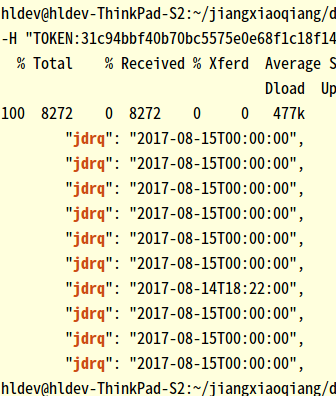
\includegraphics[scale=0.5]{grepfilterreturnvalue.png}
	\caption{Grep过滤Json结果}
	\label{fig:grepfilterreturnvalue}
\end{figure}

这样就可以轻松的看出来某个关键字段的返回结果,不需要再一个个比对。

\paragraph{sed(Stream Editor)}

sed全名叫stream editor,流编辑器,用程序的方式来编辑文本,相当的hacker啊。sed基本上就是玩正则模式匹配,所以,玩sed的人,正则表达式一般都比较强。過濾某一個時間段的日志:

\begin{lstlisting}[language=Bash]
sed -n '/^2017-08-22 18:50/','/^2017-08-22 18:59/p' cc-web.2017-08-22.0.log >> filter.log
\end{lstlisting}

-n∶取消默认的输出,使用安静(silent)模式。在一般sed的用法中,所有来自 STDIN的资料一般都会被列出到屏幕上。但如果加上 -n 参数后,则只有经过sed特殊处理的那一行(或者动作)才会被列出来。\^{}匹配一行的开始。-n选项和p命令一起使用表示只打印那些发生替换的行。

\paragraph{ag}

ag\footnote{\url{https://github.com/ggreer/the_silver_searcher}}可以递归搜索文件内容,输入如下命令安装:

\begin{lstlisting}[language=Bash]
# Ubuntu安装ag
apt-get install silversearcher-ag
dnf install the_silver_searcher
\end{lstlisting}

\paragraph{traceroute}

如果目标系统在 3 秒的超时间隔内没有响应,所有的查询都会发生超时,结果会采用星号(*)显示,由此可以断定是目标系统的问题。

\begin{lstlisting}[language=Bash]
# Linux
traceroute 10.55.10.9
# Windows
tracert 10.55.10.9
\end{lstlisting}

在traceroute输出中,收到了 ICMP\footnote{\url{https://en.wikipedia.org/wiki/Internet_Control_Message_Protocol}}错误信息(不包括时间超限和不能到达的端口),!H表示不能到达的主机。在同一局域网里面的2台主机,ping会偶尔出现丢包的情况。使用Wireshark监听ping流量如图\ref{fig:wiresharkcaptureping}所示。其中10.55.10.8表示ping主机,10.55.10.9表示目标主机。在图中提示no response found的,会在ping主机上提示“请求超时”。这里的Wireshark监听条件是host==10.55.10.8.

\begin{figure}[htbp]
	\centering
	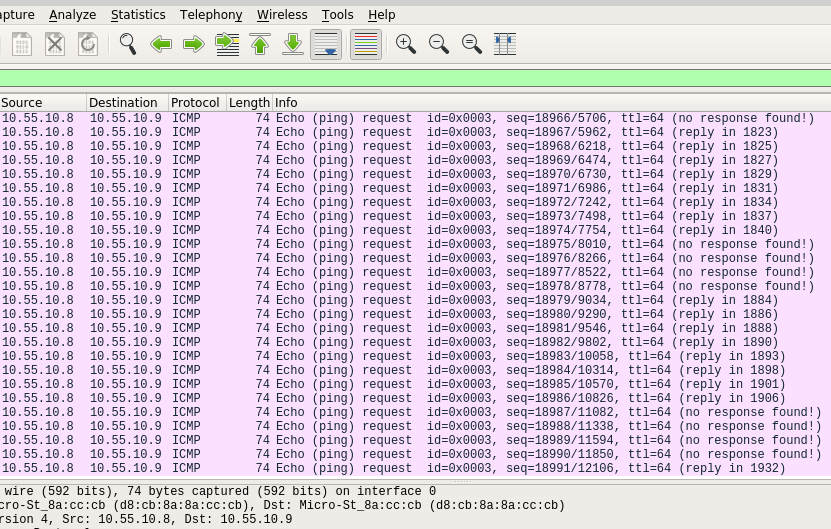
\includegraphics[scale=0.5]{wiresharkcaptureping.png}
	\caption{Wireshark监听Ping}
	\label{fig:wiresharkcaptureping}
\end{figure}

\subsection{环境变量(Environment Variable)}

Linux 分 shell变量(set),用户变量(env), shell变量包含用户变量,export是一种命令工具,是显示那些通过export命令把shell变量中包含的用户变量导入给用户变量的那些变量.删除Linux环境变量:

\begin{lstlisting}[language=Bash]
# 查看环境变量
echo $http_proxy
env
# 删除环境变量
unset http_proxy
\end{lstlisting}

set命令显示(设置)shell变量 包括的私有变量以及用户变量,不同类的shell有不同的私有变量 bash,ksh,csh每中shell私有变量都不一样。env命令显示(设置)用户变量变量。export命令显示(设置)当前导出成用户变量的shell变量。Linux profile文件如表\ref{table:linuxconfigfile}所示。

\begin{table}
	\caption{Linux profile配置文件}
	\label{table:linuxconfigfile}
	\begin{center}
	\begin{tabular}{cp{8cm}c}
		\hline
		\multirow{1}{*}{序号}
		& \multicolumn{1}{c}{名称}  \\
		\hline			
		/etc/profile  & 此文件为系统的每个用户设置环境信息,当用户第一次登录时,该文件被执行.并从/etc/profile.d目录的配置文件中搜集shell的设置 \\
		\hline	
		/etc/environment & 在登录时操作系统使用的第二个文件,系统在读取你自己的profile前,设置环境文件的环境变量 \\
		\hline
		/etc/bashrc & 为每一个运行bash shell的用户执行此文件.当bash shell被打开时,该文件被读取\\
		\hline
		~/.profile & 每个用户都可使用该文件输入专用于自己使用的shell信息,当用户登录时,该文件仅仅执行一次!默认情况下,它设置一些环境变量,执行用户的.bashrc文件\\
		\hline
		~/.bashrc &  该文件包含专用于你的bash shell的bash信息,当登录时以及每次打开新的shell时,该文件被读取\\
		\hline
	\end{tabular}	
	\end{center}
\end{table}

有时在Bash记录历史命令时,需要忽略掉重复的命令等。可以做如下设置:

\begin{lstlisting}[language=Bash]
# 忽略[连续]重复命令
HISTCONTROL=ignoredups
# 清除重复命令
# HISTCONTROL=erasedups
# 忽略特定命令
HISTIGNORE="[   ]*:ls:ll:cd:vi:pwd:sync:exit:history*"
# 命令历史文件大小10M
HISTFILESIZE=1000000000
# 保存历史命令条数10W
HISTSIZE=1000000
\end{lstlisting}

以上配置可以通过 set | grep HIST 查看可选项.当打开多个终端,关闭其中一个终端时,会覆盖其他终端的命令历史, 这里我们采用追加的方式避免命令历史文件 .bash\_history 文件被覆盖。 再次打开 ~/.bashrc 文件添加下面这一句.

\begin{lstlisting}[language=Bash]
shopt -s histappend
\end{lstlisting}

更多 shopt 可选项可以通过 echo \$SHELLOPTS 命令查看。


\subsubsection{screen}

GNU Screen是一款由GNU计划开发的用于命令行终端切换的自由软件。用户可以通过该软件同时连接多个本地或远程的命令行会话,并在其间自由切换。在使用nohup时,有一个缺点就是交互性很低,例如后台启动OpenVPN时,需要输入预先设置的认证密码。但是使用nohup命令启动时,无法显示密码输入入口。此时就需要使用screen命令了。输入如下的命令:

\begin{lstlisting}[language=Bash]
screen sudo openvpn client.conf
\end{lstlisting}

接着在跳出的窗口中,输入密码。按下Ctrl + A后再按下d键,暂时断开screen会话即可。只要Screen本身没有终止,在其内部运行的会话都可以恢复。这一点对于远程登录的用户特别有用——即使网络连接中断,用户也不会失去对已经打开的命令行会话的控制。只要再次登录到主机上执行screen -r就可以恢复会话的运行。同样在暂时离开的时候,也可以执行分离命令detach,在保证里面的程序正常运行的情况下让Screen挂起(切换到后台)。这一点和图形界面下的VNC很相似。查看当前系统中有哪些screen会话:

\begin{lstlisting}[language=Bash]
screen -ls
\end{lstlisting}

该命令会列出当前系统中所有的screen会话,重新打开会话:

\begin{lstlisting}[language=Bash]
screen -r 12865
\end{lstlisting}

正常情况下,当你退出一个窗口中最后一个程序(通常是bash)后,这个窗口就关闭了。另一个关闭窗口的方法是使用C-a k,这个快捷键杀死当前的窗口,同时也将杀死这个窗口中正在运行的进程。如果一个Screen会话中最后一个窗口被关闭了,那么整个Screen会话也就退出了,screen进程会被终止。除了依次退出/杀死当前Screen会话中所有窗口这种方法之外,还可以使用快捷键C-a :,然后输入quit命令退出Screen会话。需要注意的是,这样退出会杀死所有窗口并退出其中运行的所有程序。其实C-a :这个快捷键允许用户直接输入的命令有很多,包括分屏可以输入split等,这也是实现Screen功能的一个途径

\subsubsection{查看Linux信息}

\begin{lstlisting}[language=Bash]
# Linux查看版本当前操作系统内核信息
uname -a 
\end{lstlisting}

\section{常用设置}

\subsection{XFCE桌面}

占用资源较GNOME ,KDE较少。适合老机器,轻量级桌面。与windows界面环境类似。许多不习惯GNOME 3 ,Unity新桌面的同学,很多选择了XFCE 4.8,包括Linus大神同学。

\subsection{Fedora访问Windows共享文件夹}

在局域网里,有时需要使用Fedora 24访问Windows 7共享文件夹。在Fedora中输入命令:

\begin{lstlisting}[language=Bash]
#密码aaa321
sudo mount -t cifs -o username="aaa",uid="dolphin",gid="dolphin" //10.55.10.2/data /home/dolphin/software
\end{lstlisting}

一般提示权限错误是由于用户名密码输入错误。aaa为Windows机器的用户名,uid为当前Fedora账户的名称,gid为当前Fedora用户组的名称。10.55.10.2为Windows账户的IP,data为共享文件夹的名称,与盘符无关。/home/dolphin/software本地Fedora机器的目录。cifs为通用网络文件系统,The Common Internet File System (CIFS) is the standard way that computer users share files across corporate intranets and the Internet. An enhanced version of the Microsoft open, cross-platform Server Message Block (SMB) protocol, CIFS is a native file-sharing protocol in Windows 2000.

\subsection{Ubuntu访问Windows共享文件夹}

在Windows 7中设置了文件夹共享后,在Ubuntu文件管理器中,点击左侧的“Connect to Server”选项卡,填写Windows的IP,示例如下:

\begin{lstlisting}[language=HTML]
smb://10.55.10.2
\end{lstlisting}

点击确定后,在弹出的对话框中输入相应的用户名和密码即可。

\subsection{软件包管理(Package Management)}

根据软件包的名称模糊匹配,查看系统已经安装了哪些软件包:

\begin{lstlisting}[language=Bash]
dpkg -l|grep pcre
yum list installed|grep openssl
# 查看openssl版本
openssl version -a
# yum查看已经安装的软件包
yum list installed
# 下载指定版本软件
sudo apt-get install scala=2.12.3
# Ubuntu显示包的详细信息
sudo apt show wget
# 删除软件及其配置文件
sudo apt-get --purge -y remove <package>
\end{lstlisting}

在升级软件包的时候,可以注意软件包管理器下方的提示,在网络速度不是很理想的情况下,可以优先升级已经下载完毕后的软件包。下载软件包一个比较头疼的问题就是下载速度有时非常慢,此时如果是国外的镜像源(默认是US的镜像源),可以替换为国内的镜像源。可以直接修改/etc/apt/source.list文件和通过Software\&Updater图形界面调整。其中/etc/apt/source.list.d中存放了第三方软件的源。升级时,默认会下载服务器上最新版本的软件包,但是有时候对下载的包的版本有要求,必须是指定版本,那么可以提前查看服务器的版本,以决定是否需要下载还是手动安装:

\begin{lstlisting}[language=Bash]
# 查看服务器Scala版本
sudo apt-cache madison scala
sudo apt-cache policy scala
# 查看版本
apt-show-versions -a scala
\end{lstlisting}

madison是一个apt-cache子命令。

\subsection{Ubuntu打印}

在使用ProjectLibre撰写项目计划时,打印出来的pdf中文竟然未显示。此时需要使用虚拟打印机来打印文档了,第一步安装Linux下的虚拟打印机cups-pdf:

\begin{lstlisting}[language=Bash]
# 安装cups-pdf
sudo apt-get install cups-pdf -y --fix-missing
\end{lstlisting}

cups-pdf是Ubuntu下的PDF虚拟打印机。第二步安装ghostscript将生成的ps文件转换为pdf:

\begin{lstlisting}[language=Bash]
# 安装ghostscript包
sudo apt-get install ghostscript
# 将ps转换为pdf
ps2pdf out.ps out.pdf
\end{lstlisting}

ghostscript package contains a group of command line tools, in which ps2pdf converts .ps file to .pdf file. The package also contains other command tools, they’re dumphint, dvipdf, eps2eps, font2c, ghostscript, gs, gsbj, gsdj, gsdj500, gslj, gslp, gsnd, pdf2dsc, pdf2ps, pdfopt, pf2afm, pfbtopfa, pphs, printafm, ps2ascii, ps2epsi, ps2pdf, ps2pdf12, ps2pdf13, ps2pdf14, ps2pdfwr, ps2ps, ps2ps2, ps2txt, update-gsfontmap, wftopfa.

\subsection{输入法(Input Method)}

有时在Fedora 24中,突然中文输入法切换后无法输入中文了。可以到系统区域和语言(Region\&Language)设置界面,重新删除后再添加即可修复,如图\ref{fig:regionandlanguagesetting}所示。

\begin{figure}[htbp]
	\centering
	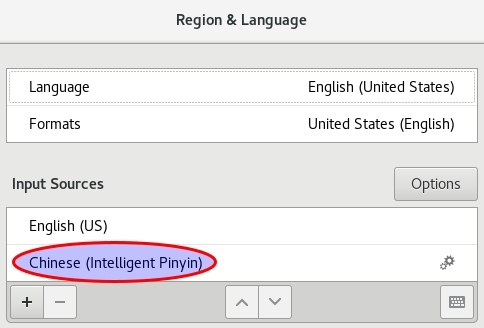
\includegraphics[scale=0.6]{regionandlanguagesetting.jpg}
	\caption{Fedora区域和语言设置}
	\label{fig:regionandlanguagesetting}
\end{figure}

在使用Ubuntu 16.04的搜狗拼音时,有时也会出现各种问题。可以尝试的解决方案包括,登录系统再次重新登入。删除输入法配置后,重新添加输入法,或者使用Google拼音输入法,输入如下命令进行安装:

\begin{lstlisting}[language=Bash]
sudo apt install fcitx-googlepinyin
\end{lstlisting}

安装好后需要重新登入系统,添加输入法配置时才可以选择Google输入法。

\newpage
~\vfil 

\part{Tool}

\newpage

\chapter{Intellij Idea}

第一次配置JDK在Configure->Project Defaults->Project Structure设置里。Mac OS X的路径一般如下:

\begin{lstlisting}[language=Bash]
# 查看Java路径
echo $JAVA_HOME
/Library/Java/JavaVirtualMachines/jdk1.8.0_112.jdk
# Mac OS X下Gradle的路径
/usr/local/Cellar/gradle/3.2.1/libexec
\end{lstlisting}

\subsection{Intellij Idea远程调试}

输入如下命令,启动远程调试:

\begin{lstlisting}[language=Bash]
nohup /home/app/local/jdk1.8.0_111/bin/java -Xmx8192M -Xms4096M -jar -Xdebug -Xrunjdwp:transport=dt_socket,suspend=n,server=y,address=5005 /home/app/backend/credit-system-web-boot-1.1.9.jar --spring.config.location=application.properties>/dev/null &
\end{lstlisting}

在远程调试Web应用时,调试时Block住了整个网站的请求,大多数时候远程调试主要是定位线上问题,调试的同时有其他人在访问,一下阻断了整个JVM肯定要不得,为了避免此种情况,可以在远程调试打断点时选择阻断当前线程而不是整个JVM,如图\ref{fig:intellijideabreakthread}所示:

\begin{figure}[htbp]
	\centering
	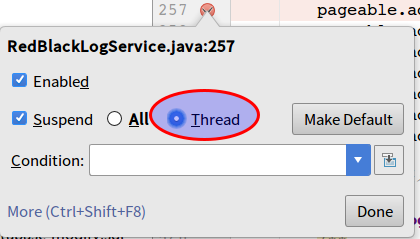
\includegraphics[scale=0.6]{intellijideabreakthread.png}
	\caption{Intellij Idea设置断点阻断当前Thread}
	\label{fig:intellijideabreakthread}
\end{figure}

这样在调试定位问题的同时,不会阻断其他用户的正常请求。

\subsection{Intellij Idea调试慢}

在使用Intellij Idea时调试Spring Boot项目时,启动时突然变慢了,原来启动10几秒,后来启动莫名其妙需要1分钟左右。经过排查是由于打了过多的断点的缘故,删除断点后,启动立即变快了。所以在项目中不能标记太多断点,调试后立即将断点删除。

\subsection{常见设置}

有时在Intellij Idea编译时找不到类,输出CLASSPATH时,发现并没有相应的Gradle库的路径在CLASSPATH中,一般使用Gradle编译时,CLASSPATH都会默认包含有.gradle路径,如:/home/hldev/.gradle/caches/modules-2/files-2.1。如果没有包含引用Library路径,可以在Project Structure->Project Settings->Libraries中添加库的路径(未解决问题)。

\begin{figure}[htbp]
	\centering
	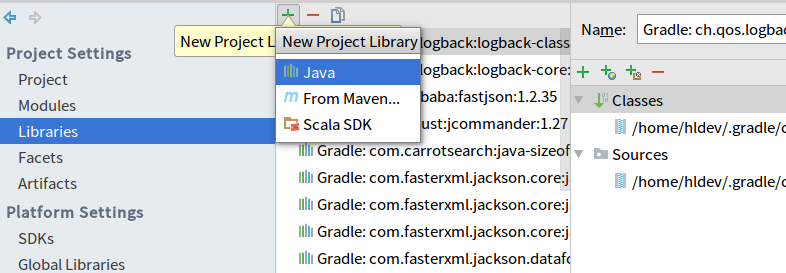
\includegraphics[scale=0.45]{intellijideaaddlibraries.png}
	\caption{Intellij Idea添加项目Library路径}
	\label{fig:intellijideaaddlibraries}
\end{figure}

也可以重新选择Gradle文件,重新导入项目(可解决问题)。

\subsection{Tips}


\begin{tabular}{cp{6cm}c}
	\hline
	\multirow{1}{*}{快捷键}
	& \multicolumn{1}{c}{作用}  \\
	\hline			
	Ctrl + Left/Right & 到行首/尾 \\
	Command + Shift + A(Mac) & Find Action \\
	Ctrl + Left/Right(Ubuntu) & 左移/右移一个单词\\
	Home/End(Ubuntu) & 光标移动到行首或者行尾\\
	Shift + Ctrl + Alt + J & Select all occurrence,选中当前单词所有出现的地方,列编辑时需要用到\\
	Alt + J & Next Occurence,上下左右搜寻,选择离当前光标最近的下一个出现的地方,按下Shift就是反向选择\\	
	\hline
\end{tabular}


\paragraph{Class JavaLaunchHelper is implemented}


启动时提示错误:

\begin{lstlisting}[language=Bash]
objc[3648]: Class JavaLaunchHelper is implemented in both /Library/Java/JavaVirtualMachines/jdk1.8.0_121.jdk/Contents/Home/bin/java (0x10d19c4c0) and /Library/Java/JavaVirtualMachines/jdk1.8.0_121.jdk/Contents/Home/jre/lib/libinstrument.dylib (0x10ea194e0). One of the two will be used. Which one is undefined.
\end{lstlisting}


检查启动配置里启动模块是否选择正确。

\paragraph{列编辑模式}

最近要做一些数据抓取转换的工作,需要编辑一些SQL脚本,突然发现可以根据SQL的注释,通过列编辑模式轻轻松松生成SQL的Insert语句。在Mac下,按住Command + Shift + Alt组合键之后,再用鼠标选择相应的区域即可。在列编辑的过程中,需要好好利用Command + Left到行首,Command + Right到行尾的功能,有时候单个字符移动光标之后,也许不是想要的光标位置,此时可以整个单词的移动,利用Alt + Left和Alt + Right快捷键。


\paragraph{自动换行}有时候,代码太长,滚动滑块不是非常方便。需要设置代码自动换行。


\paragraph{匹配文件}有时需要使用Intellij Idea的全局搜索,在匹配文件时,如果想匹配某几类文件,可以输入如下的过滤条件。

\begin{lstlisting}[language=Bash]
#在Java文件和log文件中进行匹配
*.java,*.log
\end{lstlisting}

需要同时匹配多种文件类型时,多种类型的文件以逗号隔开。

\paragraph{智能提示}

在使用Intellij Idea的过程中,有时总是不出现智能提示,不出现智能提示大致分为3种情况。其一是勾选了省电模式,在省电模式下没有智能提示。第二是缓存问题,解决办法删除缓存 file -> invalidate caches,根据提示重启Intellij Idea。 情况三配色问题。解决方法是,切换到其他配色,比如内置配色darchla。自己的是属于勾选了省电模式。

\paragraph{Template}

类模版:

\begin{lstlisting}[language=Java]
#if (${PACKAGE_NAME} && ${PACKAGE_NAME} != "")package ${PACKAGE_NAME};#end
#parse("File Header.java")
/**
* @author jiangtingqiang@gmail.com
* @create ${YEAR}-${MONTH}-${DAY}-${TIME}
*/
public class ${NAME} {
}
\end{lstlisting}



\chapter{Gradle}

一般在Mac下Gradle的安装路径为:/usr/local/Cellar/gradle/3.2.1/libexec,在Mac的Intellij Idea指定Gradle路径时,即用此路径。

\section{基础(Foundation)}

Gradle使用的Groovy语言,Groovy语言字符串的表示形式很多,有一些细微的区别:


\begin{lstlisting}
def a = '单引号形式'
def b = "双引号形式,${v}"
def c = '''三个单引号形式
支持多行
不支持占位符'''
def d = """三个双引号形式
支持多行
支持占位符,${v}"""
def e = /反斜杠形式
支持多行
支持占位符,${v}/
def f = $/美刀反斜杠形式
支持多行
支持占位符,${v}/$
\end{lstlisting}

建议使用'和"这两种形式。单引号''中的内容严格对应Java中的String,不对\$符号进行转义。双引号""的内容则和脚本语言的处理有点像,如果字符中有\$号的话,则它会\$表达式先求值。三个引号'''xxx'''中的字符串支持随意换行。

\subsection{初始化项目}

输入如下命令来初始化一个项目:

\begin{lstlisting}[language=Java]
gradle init
\end{lstlisting}

运行命令后,会在项目中新建gradlew/gradlew.bat/settings.gradle/build.gradle文件。

\subsection{引用本地文件}

有时候项目依赖的可能不是公布在网络上的一个公共库,可能只是一个闭源的jar包,只是一个本地文件而已。Gradle中引用本地文件写法如下:

\begin{lstlisting}[language=Java]
def ccDataLibs = fileTree(dir: "$rootDir/cc-data/lib", include: '*.jar')

dependencies {
	compile ccDataLibs
}
\end{lstlisting}

dir表示文件所在目录,include表示包含哪些文件。

\subsection{执行流程}

There is a one-to-one relationship between a Project and a "build.gradle" file. During build initialisation, Gradle assembles a Project object for each project which is to participate in the build, as follows:

Create a Settings instance for the build.
Evaluate the "settings.gradle" script, if present, against the Settings object to configure it.
Use the configured Settings object to create the hierarchy of Project instances.
Finally, evaluate each Project by executing its "build.gradle" file, if present, against the project. The projects are evaluated in breadth-wise order, such that a project is evaluated before its child projects. This order can be overridden by calling evaluationDependsOnChildren() or by adding an explicit evaluation dependency using evaluationDependsOn(String).

\subsection{默认JVM}

在Intellij Idea中首次导入Gradle项目时,可能提示未设置Gradle JVM,此时在项目初始选择页面选择Configure > Project Defaults > Project Structure,在项目Structure中设置JVM即可。

\subsection{repositories}

在Gradle构建标本build.gradle里,经常会看到如下脚本:

\begin{lstlisting}[language=Java]
repositories {
	maven {
		url 'http://www.eveoh.nl/files/maven2'
	}
	maven {
		url 'http://repox.gtan.com:8078'
	}
	mavenCentral()
	jcenter()
	maven { url 'http://repo.spring.io/plugins-release' }
}
\end{lstlisting}

总的来说,只有两个标准的Android library文件服务器:JCenter 和 Maven Central。起初,Android Studio 选择Maven Central作为默认仓库。如果你使用老版本的Android Studio创建一个新项目,mavenCentral()会自动的定义在build.gradle中。但是Maven Central的最大问题是对开发者不够友好。上传library异常困难。上传上去的开发者都是某种程度的极客。同时还因为诸如安全方面的其他原因,Android Studio团队决定把默认的仓库替换成JCenter。正如你看到的,一旦使用最新版本的Android Studio创建一个项目,JCenter()自动被定义,而不是mavenCentral()。mavenCentral()表示依赖是从Central Maven 2 仓库中获取的,库的地址是\url{https://repo1.maven.org/maven2}。jcenter表示依赖是从Bintary’s JCenter Maven 仓库中获取的,仓库的地址是\url{https://jcenter.bintray.com},bintray是一家提供全球企业软件开发包托管的商业公司。

\subsection{常见问题}

\paragraph{could not find method compile()}

gradle项目配置中引用java插件。

\paragraph{项目文件夹不存在}

有时在使用Gradle编译项目时,会提示项目文件夹不存在,可以使用如下命令打印项目文件夹:

\begin{lstlisting}[language=Java]
task printVarible(){
	println("rootDir:$rootDir")
	println("projectDir:$projectDir")
}
\end{lstlisting}

\section{Gradle对象}

\subsection{属性(Properties)}

\subsubsection{Extra Properties}

extra属性一般用于定义常量,All extra properties\footnote{\url{https://docs.gradle.org/current/javadoc/org/gradle/api/Project.html\#extraproperties}} must be defined through the "ext" namespace. Once an extra property has been defined, it is available directly on the owning object (in the below case the Project, Task, and sub-projects respectively) and can be read and updated. Only the initial declaration that needs to be done via the namespace.

\begin{lstlisting}[language=Java]
buildscript {
	ext {
		springBootVersion = '1.4.5.RELEASE'
		jacksonVersion = '2.8.7'
		springfoxVersion = '2.6.1'
		poiVersion = "3.14"
		aspectjVersion = '1.7.4'
	}
}
\end{lstlisting}

Reading extra properties is done through the "ext" or through the owning object.


ext.isSnapshot = version.endsWith("-SNAPSHOT")
if (isSnapshot) {
	// do snapshot stuff
}

\paragraph{定义目标jar包名}

有时在构建后需要定义目标jar包的名称。

\begin{lstlisting}[language=Java]
project(":web"){
	description = "web"
	jar{
		baseName = "dolphin-web"
	}
}
\end{lstlisting}

编译打包后的jar包名称即为dolphin-web.jar。

\subsection{Task}

对于build.gradle配置文件,当运行Gradle <Task> 时,Gradle会为我们创建一个Project的对象,来映射build.gradle中的内容。其中呢,对于不属于任何Task范畴的代码,Gradle会创建一个Script类的对象,来执行这些代码;对于Task的定义,Gradle会创建Task对象,并将它会作为project的属性存在(实际上是通过getTaskName完成的)。


\paragraph{拷贝文件}

在项目中需要根据不同的应用场景生成不同的文件,比如专门的提供外部接口的api需要单独打包,内部平台的接口需要单独打包,但是api和平台的代码都是一套代码,在一个仓库,只是配置不同罢了。此时需要Gradle在构建之后根据不同的用途生成不同的包,使用copy功能来实现。首先定义项目的动态属性:

\begin{lstlisting}[language=Java]
buildscript {
	ext {
		projectVersion = '1.1.11'
	}
}
\end{lstlisting}

然后在task中使用此属性即可。

\begin{lstlisting}[language=Java]
task copyfile(){
	println(projectVersion)
}
\end{lstlisting}

一个简单的拷贝任务,在生成完毕文件后,目的文件拷贝一个接口部署包副本,接口与应用程序单独部署,并重新命名。

\begin{lstlisting}[language=Java]
def ccCommonBuildScript = file("$rootDir/gradle/common.gradle")
apply from: ccCommonBuildScript
/**
* 复制一份接口的部署包
* 接口与平台单独部署,避免互相影响
*/
task copyTask(type: Copy) {
	from 'build/libs/credit-system-web-boot-' + version + '.jar'
	into 'build/libs/api'
	rename 'credit-system-web-boot-' + version + '.jar','credit-system-web-api-' + version + '.jar'
}
\end{lstlisting}

在这里,version变量是来自另外一个gradle文件。version变量在common.gradle中定义,在build.gradle文件中使用。


\chapter{OWASP ZAP}

\section{基础}

\subsection{调整}

OWASP消息体太长默认无法显示,可在Option/Display下调整消息体的长度。

\subsection{分析}

OWASP可以方便的保存整个网站的所有请求。

\chapter{OpenVPN}

OpenVPN从2001年开始开发,使用的是C语言。此处使用的OpenVPN版本是2.4.1。如果使用Mac下的brew工具安装,则OpenVPN目录在:/usr/local/Cellar/openvpn/2.4.1,OpenVPN的配置文件在:/usr/local/etc/openvpn。目前OpenVPN能在Solaris、Linux、OpenBSD、FreeBSD、NetBSD、Mac OS X与Microsoft Windows以及Android和iOS上运行,并包含了许多安全性的功能。此处的服务器使用的是CentOS 7.3,客户端包含Fedora 24、Ubuntu 14.04、Ubuntu 16.04、Window 7、Windows 10。在OpenVPN网络中查看存活的主机:

\begin{lstlisting}[language=bash]
nmap -A -T4 10.0.0.*
\end{lstlisting}

\subsection{安装}

安装基础包:

\begin{lstlisting}[language=bash]
sudo yum -y install openssl openssl-devel lzo openvpn easy-rsa --allowerasing
#手动安装
wget -c https://swupdate.openvpn.org/community/releases/openvpn-2.4.1.tar.gz
tar -zxvf openvpn-2.4.1.tar.gz
./configure
make && make install
\end{lstlisting}

LZO 是致力于解压速度的一种数据压缩算法,LZO 是 Lempel-Ziv-Oberhumer 的缩写。这个算法是无损算法,参考实现程序是线程安全的。 实现它的一个自由软件工具是lzop。最初的库是用 ANSI C 编写、并且遵从 GNU通用公共许可证发布的。现在 LZO 有用于 Perl、Python 以及 Java 的各种版本。代码版权的所有者是 Markus F. X. J. Oberhumer。

\subsection{生成客户端证书}

生成客户端证书端步骤如下:

\begin{lstlisting}[language=Bash]
#建立一个空的pki结构,生成一系列的文件和目录
./easyrsa init-pki
\end{lstlisting}

PKI:Public Key Infrastructure公钥基础设施。生成请求:

\begin{lstlisting}[language=Bash]
./easyrsa gen-req dolphinfedora
\end{lstlisting}

输入PEM验证码。PEM - Privacy Enhanced Mail,打开看文本格式,以"-----BEGIN..."开头, "-----END..."结尾,内容是BASE64编码。
Apache和*NIX服务器偏向于使用这种编码格式.签约:

\begin{lstlisting}[language=Bash]
#切换到服务端生成rsa的目录
#导入req
./easyrsa import-req ~/client/easyrsa/easy-rsa-master/easyrsa3/pki/reqs/dolphinfedora.req dolphinfedora
#用户签约,根据提示输入服务端的ca密码
./easyrsa sign client dolphinfedora
\end{lstlisting}

PKI:Public Key Infrastructure公钥基础设施。输入PEM验证码。PEM - Privacy Enhanced Mail,打开看文本格式,以"-----BEGIN..."开头, "-----END..."结尾,内容是BASE64编码.查看PEM格式证书的信息:openssl x509 -in certificate.pem -text -noout。Apache和*NIX服务器偏向于使用这种编码格式.服务端生成的文件有:

\begin{tabular}{|c|p{5cm}|c|}
	\hline
	\multirow{1}{*}{文件名称}
	& \multicolumn{1}{c|}{说明(Purpose)} 
	& \multicolumn{1}{c|}{位置} \\			
	\cline{1-3}
	ca.crt  & 根证书(Root CA certificate)件 & Server+All Clients	\\
	\hline
	reqs/server.req  & &\\
	\hline
	reqs/dolphin.req  & &\\
	\hline
	private/ca.key & 根证书私钥(Root CA key) & key signing machine only\\
	\hline
	private/server.key && \\
	\hline
	issued/server.crt & 服务器证书Server Certificate & server only\\
	\hline
	issued/dolphin.crt && \\
	\hline
	dh.pem & Diffie Hellman parameters & server only \\
	\hline
\end{tabular}

客户端生成的文件有:

\begin{tabular}{|c|p{8cm}|c|}
	\hline
	\multirow{1}{*}{序号}
	& \multicolumn{1}{c|}{名称}  \\			
	\cline{1-2}
	private/dolphinclient.key  & \\
	\hline
	reqs/sdolphinclient.req & \\
	\hline
\end{tabular}

拷贝出客户端证书文件:

\begin{lstlisting}[language=Bash]
cp easyrsa/easy-rsa-master/easyrsa3/pki/ca.crt ~/dolphinfedora/
cp easyrsa/easy-rsa-master/easyrsa3/pki/issued/dolphinfedora.crt ~/dolphinfedora/
cp ~/client/easyrsa/easy-rsa-master/easyrsa3/pki/private/dolphinfedora.key ~/dolphinfedora/
\end{lstlisting}


启动OpenVPN:

\begin{lstlisting}[language=Bash]
sudo openvpn server.conf
# Mac下启动OpenVPN
sudo /usr/local/Cellar/openvpn/2.4.1/sbin/openvpn /usr/local/etc/openvpn/client.conf
# 需要以后台交互方式启动时
screen sudo openvpn client.conf
\end{lstlisting}

客户端端配置如下:

\begin{lstlisting}[language=Bash]
client         #指定当前VPN是客户端
dev tun        #必须与服务器端的保持一致
proto udp      #必须与服务器端的保持一致
#指定连接的远程服务器的实际IP地址和端口号
remote 192.168.1.106 1194      
#断线自动重新连接
#在网络不稳定的情况下(例如:笔记本电脑无线网络)非常有用
resolv-retry infinite
nobind         #不绑定特定的本地端口号
persist-key
persist-tun
ca ca.crt      #指定CA证书的文件路径
cert client1.crt       #指定当前客户端的证书文件路径
key client1.key    #指定当前客户端的私钥文件路径
ns-cert-type server      #指定采用服务器校验方式
#如果服务器设置了防御DoS等攻击的ta.key
#则必须每个客户端开启;如果未设置,则注释掉这一行;
tls-auth ta.key 1     
comp-lzo              #与服务器保持一致
#指定日志文件的记录详细级别,可选0-9,等级越高日志内容越详细
verb 3                
\end{lstlisting}

配置ns-cert-type(Netscape Cert Type)指定为server主要是防止中间人攻击(Man-in-the-Middle Attack)。在服务端做如下配置:

\begin{lstlisting}[language=Bash]
nsCertType server
\end{lstlisting}

\subsection{Mac Book客户端配置}

在Mac下连接OpenVPN需要安装Tunnelblick,Tunnelblick是Mac OS X上的一个OpenVPN的图形化前端界面。Tunnelblick is free software licensed under the GNU General Public License, version 2 and may be distributed only in accordance with the terms of that license.安装好Tunnelblick之后,直接导入相应的设置即可。如下是Mac Book下一个OpenVPN客户端可用配置的示例。

\begin{lstlisting}[language=Bash]
# 定义一个客户端
client
# 和服务器保持一致
dev tun
# 用TCP协议
proto tcp
# 指定服务器的IP地址和端口,可以用多行指定多台服务器,实现负载均衡
remote 106.14.30.1 1194
;remote-random
resolv-retry infinite
# 客户端不需要绑定端口
nobind
persist-key
persist-tun
mute-replay-warnings
comp-lzo
verb 3
;mute 20
ca ca.crt
cert dolphin.crt
key dolphinclient.key
\end{lstlisting}


\subsection{Ubuntu远程Raspberry}

OpenVPN的一个应用就是可以方便的在不同局域网之间的计算机进行远程。在Raspberry安装VNC服务端:

\begin{lstlisting}[language=Bash]
sudo apt-get install tightvncserver
\end{lstlisting}

设置密码:

\begin{lstlisting}[language=Bash]
tightvncserver
\end{lstlisting}

启动:

\begin{lstlisting}[language=Bash]
vncserver :2 -geometry 800x600 -depth 24
\end{lstlisting}

在Ubuntu下远程配置如图\label{raspberryremtoeconfig}所示:

\begin{figure}[htbp]
	\centering
	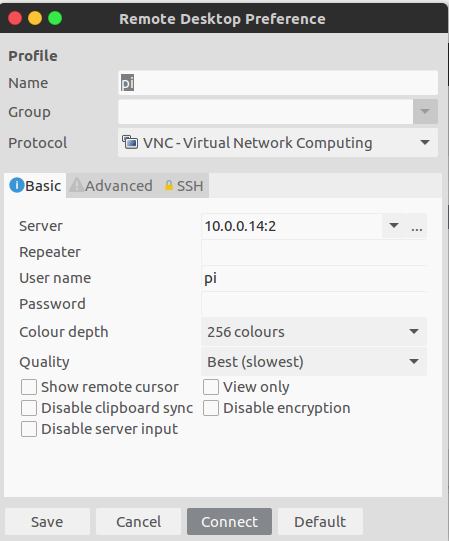
\includegraphics[scale=0.4]{raspberryremtoeconfig.png}
	\caption{Ubuntu远程连接配置}
	\label{fig:raspberryremtoeconfig}
\end{figure}

\subsection{Ubuntu远程Ubuntu}

这里的两台机器都是Ubuntu 16.04 LTS系统,xrdp支持不了13.10的GNOME了,解决办法是安装xfce界面。被远程的机器上安装必须的组件:

\begin{lstlisting}[language=Bash]
#安装xrdp
sudo apt-get install xrdp -y
#安装vnc4server
sudo apt-get install vnc4server tightvncserver -y
#安装xfce4
sudo apt-get install xubuntu-desktop -y
sudo /etc/init.d/xrdp restart
# 指定桌面管理器
echo "gnome-session --session=gnome-classic" > ~/.xsession
\end{lstlisting}

最后一个命令的作用是由于安装了gnome桌面,ubuntu16.04中同时存在unity、GNOME多个桌面管理器,需要启动的时候指定一个,不然即使远程登录验证成功以后,也只是背景。在Ubuntu上使用Remmina Remote Desktop Client即可链接远程桌面。

\subsection{Mac Book远程Fedora}

在Mac Book远程Linux主机选择的是XQuartz,安装好XQuartz后,直接在从XQuartz打开的终端中运行:

\begin{lstlisting}[language=Bash]
ssh -X dolphin@10.0.0.10
\end{lstlisting}

直接在命令行中启动图形化界面,会在Mac上显示Linux主机上的软件原生GUI界面,就像软件在本机运行一样。X11是X Window System主版本11的缩写,它不光是一个基本的GUI软件,X11也被定义为一个网络协议,因为X11提供了非常灵活的网络访问接口。SSH 的 X11 forwarding 特性可以使 X client 和 X server 安全地通讯。使用 X11 forwarding 后,从 X client 到 X Server 方向的数据先被送至 SSH server,SSH server 利用和 SSH client 的安全通道转发给 SSH client,再由 SSH client 转发给 X server,从 X server 到 X client 的数据流同理。这里 SSH server 和 SSH client 充当了 X client 和 X server 间数据的转发器,由于 SSH server 和 X client、SSH client 和 X server 一般在同一台机器上,它们之间是一种安全的进程间通讯,而 SSH server 和 SSH client 间的通讯也是安全的,所以 X client 和 X server 间的通讯就是安全的。X在Unix-like系统上几乎完全占据统治地位。但是仍然有人尝试提供替代品和更多的选择,过去曾经有 Sun Microsystems 的 NeWS ,但它遭到市场失败;还有 NeXT 的 Display PostScript ,它最终转变为苹果电脑的 Quartz for Mac OS X 。

\subsection{常见问题}

得到了Initialization Sequence Completed消息,但是ping失败了 -- 这通常是服务端或客户端上的防火墙过滤了TUN/TAP网络接口从而阻止了VPN网络的流量。  

\subsubsection{ssl3\_get\_server\_certificate:certificate verify failed}

在Mac中,连接好了并没有显示IP的变化。This computer's apparent public IP address was not different after connecting to client. It is still 45.76.205.201.This may mean that your VPN is not configured correctly.


\paragraph{OpenVPN is connected to the server but your IP address does not change}

If OpenVPN connects to the server properly but your IP address does not change, you are probably missing the "--redirect-gateway" option. Add the following line:
--redirect-gateway def1 to your configuration file.

By default, OpenVPN only sends some traffic through the VPN — traffic that is specifically destined for the VPN network itself. The "--redirect-gateway" option tells OpenVPN to send all traffic through the VPN. (Leave out the "--" when it is put in the configuration file.)

An alternative to putting "redirect gateway def1" in the configuration file is to "push" it from the VPN server to the client.

\chapter{Nmap(GNU General Public License)}

Nmap(Network Mapper),网络映射器,是一款开放源代码的网络探测和安全审核的工具。
它的设计目标是快速地扫描大型网络,当然用它扫描单个主机也没有问题。
Nmap以新颖的方式使用原始IP报文来发现网络上有哪些主机,
那些主机提供什么服务(应用程序名和版本),那些服务运行在什么操作系统(包括版本信息),
它们使用什么类型的报文过滤器/防火墙,以及一堆其它功能。虽然Nmap通常用于安全审核,
许多系统管理员和网络管理员也用它来做一些日常的工作,比如查看整个网络的信息,
管理服务升级计划,以及监视主机和服务的运行。
Nmap脚本引擎(Nmap Script Engine)是Nmap最有力灵活的的一个特性。
它允许用户撰写和分享一些简单的脚本来一些较大的网络进行扫描任务。
基本上这些脚本是用Lua编程语言来完成的。通常Nmap的脚本引擎可以完成很多事情。

\subsection{主机发现(Host Discovery)}

主机发现顾名思义就是发现所要扫描的主机是否是正在运行的状态。
输入如下命令开始主机扫描

\begin{lstlisting}[language=Bash]
nmap -F -sT -v nmap.org
# 主机发现,生成存活主机列表
nmap -sn -T4 -oG Discovery.gnmap 192.168.24.0/24
grep "Status: Up" Discovery.gnmap | cut -f 2 -d ' ' > LiveHosts.txt
\end{lstlisting}

\begin{itemize}
	\item{-F}扫描100个最有可能开放的端口,F表示快速模式(Fast Model),
	比默认模式扫描更少的端口(Scan fewer ports than the default scan),
	如果需要扫描更多的端口,指定p参数,如下命令行片段所示:
	
\begin{lstlisting}[language=Bash]
nmap -p 0-10000 -A -v <Host>
\end{lstlisting}
	
	端口号最好分段指定,否则扫描的速度会非常缓慢,
	例如需要扫描0-65535端口,可以先扫描0-10000端口,
	再扫描10001-20000,依次类推。
	
	\item{-v}获取扫描的信息
	\item{-sT(Scan using TCP)}采用的是TCP扫描,不写也是可以的,默认采用的就是TCP扫描
	\item{-sn参数表示ping扫描,禁用端口扫描}
	\item{-oG表示输出Grepable格式}
\end{itemize}

Nmap输出的是扫描目标的列表,以及每个目标的补充信息,至于是哪些信息则依赖于所使用的选项。
“所感兴趣的端口表格”是其中的关键。那张表列出端口号,协议,服务名称和状态。
状态可能是 open(开放的),filtered(被过滤的), closed(关闭的),或者unfiltered(未被过滤的)。
Open(开放的)意味着目标机器上的应用程序正在该端口监听连接/报文。 
filtered(被过滤的) 意味着防火墙,过滤器或者其它网络障碍阻止了该端口被访问,
Nmap无法得知 它是 open(开放的) 还是 closed(关闭的)。 
closed(关闭的) 端口没有应用程序在它上面监听,但是他们随时可能开放。 
当端口对Nmap的探测做出响应,但是Nmap无法确定它们是关闭还是开放时,
这些端口就被认为是 unfiltered(未被过滤的) 如果Nmap报告状态组合 
open|filtered 和 closed|filtered时,那说明Nmap无法确定该端口处于两个状态中的哪一个状态。
当要求进行版本探测时,端口表也可以包含软件的版本信息。
当要求进行IP协议扫描时 (-sO),Nmap提供关于所支持的IP协议而不是正在监听的端口的信息。
获取远程主机的系统类型及开放端口:

\begin{lstlisting}[language=Bash]
nmap -sS -P0 -sV -O <target>
\end{lstlisting}

\subsection{端口扫描(Port Scanning)}

端口扫描是Nmap最基本最核心的功能,用于确定目标主机的TCP/UDP端口的开放情况。
端口扫描简单示例如下代码片段所示:

\begin{lstlisting}[language=Bash]
#服务扫描
nmap-T4 -sV targetip 

#扫描淘宝IP
nmap -p 0-1000 -v 218.201.46.124
nmap -T4 -A -v 218.201.46.124

# 扫描指定主机的3306端口
nmap -sS -p 3306 -v 192.168.31.25
\end{lstlisting}

通过扫描可以发现一些主机信息,比如淘宝的数字证书用的是GlobalSign,
加密位数是2048,签名算法是sha256WithRSAEncryption,
操作系统猜测是Linux系列的,内核版本可能是3.X或者2.6.X,
具体信息如下。

\begin{lstlisting}
443/tcp open  ssl/http Tengine httpd
|_http-server-header: Tengine
|_http-title: 501 Not Implemented
| ssl-cert: Subject: commonName=*.tmall.com/organizationName=Alibaba (China) Technology Co., Ltd./stateOrProvinceName=ZheJiang/countryName=CN
| Issuer: commonName=GlobalSign Organization Validation CA - SHA256 - G2/organizationName=GlobalSign nv-sa/countryName=BE
| Public Key type: rsa
| Public Key bits: 2048
| Signature Algorithm: sha256WithRSAEncryption
| Not valid before: 2015-12-14T10:38:38
| Not valid after:  2016-12-14T10:38:38
| MD5:   5d67 3ca3 7f0e 2ab7 7b4f 59d5 0700 7223
|_SHA-1: d048 e9cf 5487 5030 9f26 e638 7d3f 94ad a2b3 e6fa
\end{lstlisting}

默认情况下,Nmap会扫描1000个最有可能开放的TCP端口。

1)公认端口(0~1023),又称常用端口,为已经公认定义或为将要公认定义的软件保留的。
这些端口紧密绑定一些服务且明确表示了某种服务协议。如80端口表示HTTP协议。
2)注册端口(1024~49151),又称保留端口,这些端口松散绑定一些服务。
3)动态/私有端口(49152~65535)。理论上不应为服务器分配这些端口。
按协议类型可以将端口划分为TCP和UDP端口。
1)TCP端口是指传输控制协议端口,需要在客户端和服务器之间建立连接,
提供可靠的数据传输。如Telnet服务的23端口。
2)UDP端口是指用户数据包协议端口,不需要在客户端和服务器之间建立连接。
常见的端口有DNS服务的53端口。
有的服务器为了安全会修改默认端口,
比如将ssh默认的22端口修改为50000,
不过通过Nmap扫描也会很容易的发现。
详细的扫描指令如下所示:

\begin{lstlisting}[language=Bash]
nmap -sS -sU -T4 -A -v -PE -PP -PS80,443 -PA3389 -PU40125 -PY -g 53 --script "default or (discovery and safe)" 12.26.32.14 
\end{lstlisting}

\begin{itemize}
	\item{-sS参数(TCP SYN Scan)可以利用基本的SYN扫描方式探测其端口开放状态}
	\item{-sU参数代表UDP Scan}
	\item{-T<0-5>: Set timing template (higher is faster)}
	\item{-A: Enable OS detection, version detection, script scanning, and traceroute}
	\item{-v: Increase verbosity level (use -vv or more for greater effect)}
	\item{-PE/PP/PM: ICMP echo, timestamp, and netmask request discovery probes}
	\item{-PS/PA/PU/PY[portlist]: TCP SYN/ACK, UDP or SCTP discovery to given ports}
	\item{-g/--source-port <portnum>: Use given port number}
\end{itemize}


\paragraph{"ppp0" is not an ethernet device}在使用nmap扫描时候,提示 

\begin{lstlisting}
Only ethernet devices can be used for raw scans on Windows, and "ppp0" is not an ethernet device. Use the --unprivileged option for this scan. QUITTING!
\end{lstlisting}

因为用Nmap扫描时,不能用pppoe的拨号口,只能用以太网口。
根据提示带参数--unprivileged就可以了,注意扫描的命令不能带-A参数,
否则会要求root权限,无法启动扫描。 


\subsection{版本侦测(Version Detection)}

版本侦测在后面添加sV(Service/Version)参数即可。

\begin{lstlisting}[language=Bash]
-sV: Probe open ports to determine service/version info
\end{lstlisting}

\subsection{Zenmap}

Zenmap是Nmap的官方GUI,可以运行在Linux, Windows, Mac OS X, BSD等操作系统上。

\begin{lstlisting}[language=Bash]
# Mac下获取Zenmap安装文件
wget -c https://nmap.org/dist/nmap-7.31.dmg
\end{lstlisting}


\section{tmux}

tmux是一个优秀的终端复用软件,类似GNU Screen,但来自于OpenBSD,采用BSD授权。使用tmux的好处之一就是可以保存会话,避免网络不稳定带来的影响。

\begin{tabular}{|c|p{8cm}|c|}
	\hline
	\multirow{1}{*}{键}
	& \multicolumn{1}{c|}{作用}  \\			
	\cline{1-2}
	Ctrl + b d  & 返回主 shell ,detach, tmux 依旧在后台运行,里面的命令也保持运行状态\\
	\hline
	C-b ? & 显示快捷键帮助\\
	\hline
\end{tabular}


\chapter{Raspberry Pi}

\section{基础}

\subsection{连接(Connection)}

Raspberry可以通过网线直接与PC连接,输入如下命令查看Raspberry的IP:

\begin{lstlisting}[language=Bash]
arp -a
\end{lstlisting}

初次登录需要通过有线连接,设置完成后,如果是连接的是隐藏网络,有可能无线无法获取IP.此时网络设置需要添加scan\_ssid:

\begin{lstlisting}[language=Bash]
network={
  ssid="爱生活"
  scan_ssid=1
  psk="15023396614"
  priority=3
}
\end{lstlisting}

SSID是个笼统的概念,包含了ESSID和BSSID,用来区分不同的网络,最多可以有32个字符,无线网卡设置了不同的SSID就可以进入不同网络,SSID通常由AP广播出来,通过XP自带的扫描功能可以查看当前区域内的SSID。出于安全考虑可以不广播SSID,此时用户就要手工设置SSID才能进入相应的网络。简单说,SSID就是一个局域网的名称,只有设置为名称相同SSID的值的电脑才能互相通信。

检查配置文件是否有错误:

\begin{lstlisting}[language=Bash]
sudo wpa_supplicant -c /etc/wpa_supplicant/wpa_supplicant.conf  -i wlan0
\end{lstlisting}

安装步骤:

\begin{lstlisting}[language=Bash]
# 安装tightvncserver
sudo apt-get install tightvncserver -y
# 设置密码
vncpasswd
\end{lstlisting}

Raspberry Pi的网络配置,需要编辑/etc/wpa\_supplicant/wpa\_suppliant.conf文件。编辑后重启网络:

\begin{lstlisting}[language=Bash]
/etc/init.d/networking restart
\end{lstlisting}

\chapter{Widgets}

\section{Little Tool}

\subsection{transmission}

在使用磁力链接下载元素据时,如果下载时间太长,一般是网络的问题,电信的网络普遍优于长城等。

\subsection{rsync}

rsync命令是一个远程数据同步工具,可通过LAN/WAN快速同步多台主机间的文件。rsync使用所谓的“rsync算法”来使本地和远程两个主机之间的文件达到同步,这个算法只传送两个文件的不同部分,而不是每次都整份传送,因此速度相当快。使用一个远程shell程序(如rsh、ssh)来实现将本地机器的内容拷贝到远程机器。当DST路径地址包含单个冒号":"分隔符时启动该模式。

\begin{lstlisting}[language=Bash]
rsync -avz pi@10.42.0.22:app-soft .
\end{lstlisting}



\subsection{ag}

silversearcher-ag可递归搜索文件内容。

\begin{lstlisting}[language=Bash]
apt-get install silversearcher-ag
\end{lstlisting}

\subsection{Pandoc}

Pandoc使用haskell开发的一个文档格式转换软件。在编写文档时习惯使用\LaTeX{}来编写,\LaTeX{}生成的pdf文档美观,Word格式在不同平台(Mac OS X/Linux/Windows)不同的软件(Microsft Office/金山/Libre Office)打开格式可能会不一致,但是有许多同事习惯使用Word,有时发给对方时也需要作一些编辑和调整,Pandoc就可以满足既可以用\LaTeX{}来编辑文档,也可以将Tex文档转换为Word方便同事:

\begin{lstlisting}[language=Bash]
pandoc -s interface.tex -o example30.docx
\end{lstlisting}

另外使用\LaTeX{}还有一个比较方便的地方是可以容易的以模块来管理文档,比如接口文档分为公共部分,所有调用方都可以看到,但是针对每个调用方可能会有一些定制的内容,当要修改公共部分时,如果是采用Word文件分散管理会出现不一致的情况,有的文件修改了,有的没有改。使用\LaTeX{}就只需要改动一个公共模块即可。其他引用公共的地方自动更新。

\subsection{Curl}

内部接口测试:

\begin{lstlisting}[language=Bash]
curl -i -H "APPID:hlb1451j6d136334gh2" \ 
-H "ECHOSTR:sdsaasf" \
-H "TOKEN:e02016ed4adfda9d9743ab70cf389ef9877c4a0e" \
-H "TIMESTAMP:2016-12-19 16 (tel:2016121916):58:02" http://localhost:28080/api/article
\end{lstlisting}

使用如下命令上传文件:

\begin{lstlisting}[language=Bash]
curl -i -X POST -F "filename=@example.tar.gz;filename1=@example1.tar.gz" http://localhost:28080/api/article
curl -i -X POST host:port/post-file -H "Content-Type: text/xml" --data-binary "@path/to/file"
# 使用curl將文件上傳到服務器,文件類型可以任意
curl -i -X POST -H "APPID:hlb1451j6d136334gh2" \
-H "ECHOSTR:sdsaasf" \
-H "TOKEN:e02016ed4adfda9d9743ab70cf389ef9877c4a0e" \
-H "TIMESTAMP:2016-12-19 16 (tel:2016121916):58:02" \
-F "upfile=@main.synctex.gz" http://localhost:28080/api/article
\end{lstlisting}

The -i option tells curl to show the response headers as well。如果使用了-F参数,curl就会以 multipart/form-data的方式发送POST请求。-F参数以name=value的方式来指定参数内容,如果值是一个文件,则需要以name=@file的方式来指定。文件的路径需要有一个@符号,所以curl知道从文件中读取。upfile對應服務端的方法參數。有时需要查看接口详细的响应时间,采用如下命令:

\begin{lstlisting}[language=Bash]
# 文件curl-format.txt写入的内容
time_namelookup:  %{time_namelookup}\n
time_connect:  %{time_connect}\n
time_appconnect:  %{time_appconnect}\n
time_pretransfer:  %{time_pretransfer}\n
time_redirect:  %{time_redirect}\n
time_starttransfer:  %{time_starttransfer}\n
----------\n
time_total:  %{time_total}\n

curl -w "@curl-format.txt" -s -H "APPID:" \
-H "TIMESTAMP:2016-12-19 16 (tel:2016121916):58:02" \
-H "ECHOSTR:sdsaasf" -H "TOKEN:" \
-H "Accept: application/json, text/plain" \
http://localhost:28080/api/xysj/search?qymc=长安福特
\end{lstlisting}


\subsection{iostat}

查看磁盘的IO情况,每秒刷新一次:

\begin{lstlisting}[language=Bash]
iostat 2 -cdxk
\end{lstlisting}

参数 -d(Device)表示,显示设备(磁盘)使用状态;-k某些使用block为单位的列强制使用Kilobytes为单位;2表示,数据显示每隔2秒刷新一次。iostat还有一个比较常用的选项-x,该选项将用于显示和io相关的扩展数据。-c用来获取cpu部分状态值。为显示更详细的io设备统计信息,可以使用-x选项。

\subsection{Zeal}

Zeal是一个离线的文档浏览工具。查看Nginx Stream相关文档信息,示例如图\ref{fig:zealsearch}所示。搜索以nginx和冒号开始,表示搜索与Nignx相关的信息。

\begin{figure}[htbp]
	\centering
	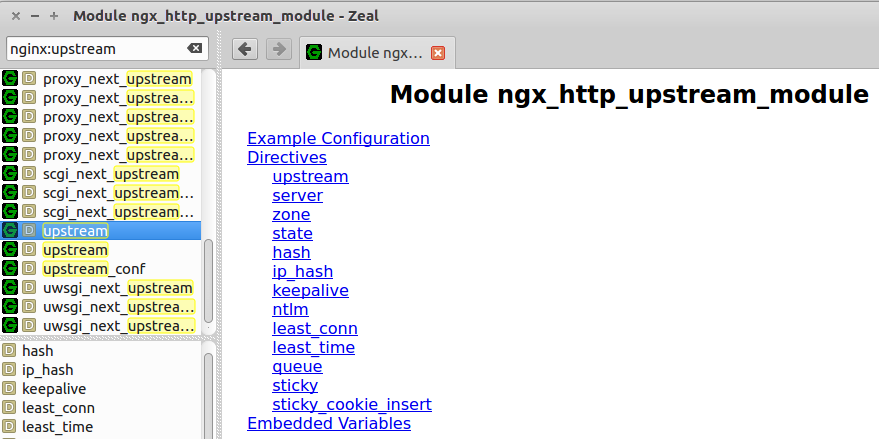
\includegraphics[scale=0.4]{zealsearch}
	\caption{Zeal文档搜索示例}
	\label{fig:zealsearch}
\end{figure}

\subsection{jq}

项目里同事根据接口返回的数据建立数据库表格时,需要看格式化后的Json,由于只能在终端中请求接口数据,未格式化的Json返回根本没法阅读。由于目前还未发现Json格式化工具,所以只能时粘贴Json到网络上的在线网页里面进行格式化,由于网络用的是物理隔离的内网,甭提有多麻烦了,而且都是重复劳动,而jq采用C语言编写(开始还以为是用Python写的),没有运行时依赖(jq is written in portable C, and it has zero runtime dependencies.),直接在服务器上源码编译安装即可(服务器物理隔离,只能源码安装)。没有它,估计耗费的时间不下几个小时。jq直接在终端中就可以查看格式化好的Json。需要说明的是 jq 只能接受 well form 的 JSON 字符串作为输入内容。也就是说输入内容必须严格遵循 JSON 格式的标准。所有的属性名必须是以双引号包括的字符串。对象的最后一个属性的末尾或者数组的最后一个元素的末尾不能有逗号。否则 jq 会抛出无法解析 JSON 的错误。


\paragraph{常用模式}

获取所有的key:

\begin{lstlisting}[language=Bash]
echo '{"foo": 42, "bar": "less interesting data"}' | jq 'keys'
# 获取某一个value的值
echo '{"foo": 42, "bar": "less interesting data"}' | jq '.bar'
\end{lstlisting}

嵌套数据查看:

\begin{lstlisting}[language=Bash]
curl -H "APPID:" -H "TIMESTAMP:2016-12-19 16 (tel:2016121916):58:02" -H "ECHOSTR:" -H "TOKEN:" http://10.10.1.12:28080/api/xzxk?xdr= | jq '.data.totalElements'
\end{lstlisting}

\section{Nginx}

安装配置好nginx服务器后默认目录是/usr/share/nginx/html。nginx模块一般被分成三大类:handler、filter和upstream。Mac下Nginx配置文件的路径为:/usr/local/etc/nginx/nginx.conf。

\subsection{X-Forwarded-For}

X-Forwarded-For是一个HTTP扩展头部。HTTP/1.1(RFC 2616)协议并没有对它的定义,它最开始是由 Squid 这个缓存代理软件引入,用来表示 HTTP 请求端真实 IP。如今它已经成为事实上的标准,被各大 HTTP 代理、负载均衡等转发服务广泛使用,并被写入 RFC 7239(Forwarded HTTP Extension)标准之中。在默认情况下,Nginx并不会对X-Forwarded-For头做任何的处理,除非用户使用proxy\_set\_header参数设置:

\begin{lstlisting}[language=bash]
proxy_set_header X-Forwarded-For $proxy_add_x_forwarded_for;
\end{lstlisting}

X-Forwarded-For 请求头格式:

\begin{lstlisting}[language=bash]
X-Forwarded-For: IP0, IP1, IP2
\end{lstlisting}

XFF 的内容由「英文逗号 + 空格」隔开的多个部分组成,最开始的是离服务端最远的设备 IP,然后是每一级代理设备的 IP。

\subsection{Nginx获取真实IP}

做异地登陆的判断,或者统计ip访问次数等,通常情况下我们使用request.getRemoteAddr()就可以获取到客户端ip,但是当我们使用了nginx作为反向代理后,使用request.getRemoteAddr()获取到的就一直是nginx服务器的ip的地址。Nginx作为HTTP代理转发前端时,后端服务无法获知前端访问客户的IP地址。要获取客户端IP,需要将http\_realip\_module编译进入Nginx中。查看Nginx安装了哪些模块,使用如下命令:

\begin{lstlisting}[language=bash]
nginx -V
\end{lstlisting}

在命令的输出结果中,可以看到Nginx的版本,Nginx的编译参数,和Nginx已经包含有哪些模块。此处显示已经编译了http\_realip\_module模块。在服务器上的项目中使用的tengine,经过查看是没有编译http\_realip\_module模块,从tengine官网上下载好源码,输入如下命令进行编译:

\begin{lstlisting}[language=bash]
# 在Ubuntu 14.04 LTS下安装pcre依赖
# pcre:Perl Compatible Regular Expressions
sudo apt-get install libpcre3 libpcre3-dev
# 指定预编译参数,仅仅指定路径
sudo ./configure --prefix=/opt/tengine
# 将realip模块编译进入
sudo ./configure --prefix=/opt/tengine --with-http_realip_module
# 编译
sudo make
# 安装
sudo make install
./configure --prefix=/usr/local/tengine-2.1.2 --with-openssl=/Users/dolphin/source/openssl
\end{lstlisting}

不指定prefix,则可执行文件默认放在/usr/local/bin,库文件默认放在/usr/local/lib,配置文件默认放在/usr/local/etc。其它的资源文件放在/usr /local/share。
你要卸载这个程序,要么在原来的make目录下用一次make uninstall(前提是make文件指定过uninstall),要么去上述目录里面把相关的文件一个个手工删掉。
指定prefix,直接删掉一个文件夹就够了,这也是制定prefix一个比较方便的地方。在编译时,还需要指定pcre的版本,因为Ubuntu 16.04 LTS里有时安装有pcre 3,而部署的电脑上不一定安装有pcre 3,而且pcre 3的源码不容易找到。所以编译命令如下:

\begin{lstlisting}[language=bash]
# 将realip模块编译进入,并指定pcre
sudo ./configure --prefix=/opt/tengine --with-http_realip_module --with-pcre=/root/software/pcre-8.40 --with-openssl=/root/software/openssl-OpenSSL_1_1_0e --without-http_gzip_module

./configure --prefix=/opt/tengine --with-http_realip_module --with-pcre=/root/software/pcre-8.40  --without-http_gzip_module

#本机编译(不成功)
./configure --prefix=/opt/tengine --with-http_realip_module --with-pcre=/home/hldev/Downloads/pcre-8.40 --with-openssl=/home/hldev/Downloads/openssl-OpenSSL_1_0_1e --without-http_gzip_module

#本机编译(成功)
-prefix=/opt/tengine --with-http_realip_module --with-pcre=/home/hldev/Downloads/pcre-8.40 --with-openssl=/home/hldev/software/openssl-OpenSSL_1_0_2g --without-http_gzip_module

# 构建程序
make

#安装程序
make install

#服务器
./configure --prefix=/opt/tengine

./configure: error: SSL modules require the OpenSSL library.
You can either do not enable the modules, or install the OpenSSL library
into the system, or build the OpenSSL library statically from the source
with nginx by using --with-openssl=<path> option.


\end{lstlisting}

其中--with-pcre表示pcre(Perl Compatible Regular Expressions)的源代码目录。在编译时,还需要注意openssl的版本,本地电脑版本是1.0.2g,服务端的版本是1.0.1e。服务器端编译Nginx的一个命令:

\begin{lstlisting}[language=bash]
./configure --prefix=/opt/tengine --with-openssl=/usr/local/src/openssl-OpenSSL_1_0_2g/ --without-http_gzip_module --with-pcre=/usr/local/src/pcre-8.40/
\end{lstlisting}

这里编译的时候有一个小细节需要注意,需要将源码包存放到/usr/local/src目录下。一直没有编译成功也许是这个小小的细节,开始时是将源码包随意存放的一个目录。以上编译的命令没有包含Zlib,也没有包含http\_realip\_module模块。最终的编译命令如下:

\begin{lstlisting}[language=bash]
./configure --prefix=/opt/tengine --with-openssl=/usr/local/src/openssl-OpenSSL_1_0_2g/ --with-pcre=/usr/local/src/pcre-8.40/ --with-zlib=/usr/local/src/zlib-1.2.11 --with-http_realip_module 
\end{lstlisting}

编译完毕之后,输入如下命令:

\begin{lstlisting}[language=bash]
# 查看Tengine版本、模块信息,编译时所使用的参数
./nginx -V
\end{lstlisting}

即可看到http\_realip\_module已经编译到Nginx中了。Nginx的http realip module等于Apache的mod\_rpaf,用于接受前端发来的IP head信息,从获取到真实的用户IP。将获取真实IP的模块编译进入Nginx后,还需要在对应的http、server、location中加入以下参数:

\begin{lstlisting}[language=bash]
#指令是告诉nginx,10.10.1.11是我们的反向代服务器
#不是真实的用户IP
set_real_ip_from 10.10.1.11;
#告诉nginx真正的用户IP是存在X-Forwarded-For请求头中
real_ip_header X-Real-IP;
\end{lstlisting}

其中set\_real\_ip\_from可以指定某个网段。这个指令指定信任的代理IP,它们将会以精确的替换IP转发。0.8.22后可以指定Unix sockets。real\_ip\_header设置需要使用哪个头来确定替换的IP地址。由于项目中使用的Nginx作为反向代理,所以配置如下:

\begin{lstlisting}[language=bash]
location /inapi {
proxy_pass http://localhost:28080;
proxy_set_header X-Real-IP $remote_addr;
proxy_redirect off;
}
\end{lstlisting}

在另一台电脑上访问服务端,在后端根据新添加的Header获取到的IP地址如图\ref{fig:nginxgetrealip}所示:

\begin{figure}[htbp]
	\centering
	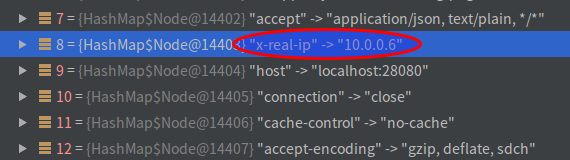
\includegraphics[scale=0.6]{nginxgetrealip.png}
	\caption{Nginx获取用户真实访问IP}
	\label{fig:nginxgetrealip}
\end{figure}

此处获取到的IP是用户的真实IP,而不是反向代理服务器的IP。

\subsection{Nginx并发}

如何设置能限制某个IP某一时间段的访问次数是一个让人头疼的问题,特别面对恶意的ddos攻击的时候。其中CC攻击(Challenge Collapsar)是DDOS(分布式拒绝服务)的一种,也是一种常见的网站攻击方法,攻击者通过代理服务器或者肉鸡向向受害主机不停地发大量数据包,造成对方服务器资源耗尽,一直到宕机崩溃。

cc攻击一般就是使用有限的ip数对服务器频繁发送数据来达到攻击的目的,nginx可以通过HttpLimitReqModul和HttpLimitZoneModule配置来限制ip在同一时间段的访问次数来防cc攻击。

HttpLimitReqModule用来限制连单位时间内连接数的模块,使用limit\_req\_zone和limit\_req指令配合使用来达到限制。一旦并发连接超过指定数量,就会返回503错误。limit\_req\_zone 用来限制单位时间内的请求数,即速率限制,采用的漏桶算法 “leaky bucket”。

\begin{lstlisting}[language=bash]
http {
	limit_conn_log_level error;
	limit_conn_status 503;
	#Zone=one或allips表示设置了
	#名为“one”或“allips”的存储区
	#大小为10兆字节
	limit_conn_zone $binary_remote_addr zone=one:10m;
	limit_conn_zone $server_name zone=perserver:10m;
	#rate=10r/s 的意思是允许1秒钟不超过1000个请求
	limit_req_zone $binary_remote_addr zone=allips:100m rate=1000r/s;  
	server {
		limit_conn one 100;
		limit_conn perserver 3000;
		limit_req zone=allips  burst=5  nodelay;
	}
}
\end{lstlisting}

HttpLimitConnModule用来限制单个ip的并发连接数,使用limit\_zone和limit\_conn指令,这两个模块的区别前一个是对一段时间内的连接数限制,后者是对同一时刻的连接数限制。

\subsection{URI长度限制}

在Http1.1协议中并没有提出针对URL的长度进行限制,RFC协议里面是这样描述的,HTTP协议并不对URI的长度做任何的限制,服务器端必须能够处理任何它们所提供服务多能接受的URI,并且能够处理无限长度的URI,如果服务器不能处理过长的URI,那么应该返回414状态码。接触的最多的服务器类型就是Nginx和Tomcat,对于url的长度限制,它们都是通过控制http请求头的长度来进行限制的,nginx的配置参数为large\_client\_header\_buffers,tomcat的请求配置参数为maxHttpHeaderSize。

\begin{lstlisting}[language=bash]
# Nginx配置HTTP请求头长度
client_header_buffer_size 2048k;
\end{lstlisting}

项目采用Spring Boot,所使用的Tomcat为内嵌的Tomcat。在application.properties中,增加如下配置:

\begin{lstlisting}[language=bash]
#单位为KB,如果没有指定,默认为8192(8KB)
server.max-http-header-size=1024
\end{lstlisting}

奇怪的是,在本机设置的1024KB可以查询,部署到服务器上,参数必须再调大才能够查询,否则提示请求头太大的错误。真的遇到鬼了。在不同的操作系统上单位不一样吗?见鬼

\subsection{开启gzip压缩}

Nginx开启Gzip压缩配置如下:

\begin{lstlisting}[language=Bash]
gzip on;
gzip_min_length 1k;
gzip_buffers 4 16k;
gzip_comp_level 2;
gzip_types application/javascript application/json text/plain application/x-javascript text/css application/xml text/javascript application/x-httpd-php image/jpeg image/gif image/png;
gzip_vary off;
gzip_disable "MSIE [1-6]";
\end{lstlisting}

用curl测试是否开启了压缩:

\begin{lstlisting}[language=Bash]
curl -I -H "Accept-Encoding: gzip, deflate" "http://creditsystem.test/main"
curl -I -H "Accept-Encoding: gzip, deflate" "http://10.10.1.11/main"
\end{lstlisting}

-I选项与-header选项是等价的,表示只打印出HTTP头部。开启压缩成功后,可以看到一句:Content-Encoding: gzip。

\subsection{Nginx配置}

简单的配置:

\begin{lstlisting}[language=bash]
user www-data;
worker_processes 4;
pid /run/nginx.pid;

events {
	worker_connections 768;
}

http {
	server{
		listen 80;
		# 定义网站默认根目录
		root /opt/dolphin/frontend/dist;
		
		location /api {
			proxy_pass http://localhost:8011;
		}
		
		location / {
			root /opt/dolphin/frontend/dist;
			index index.html;
		} 
	}
}
\end{lstlisting}

\subsection{常见问题}

\paragraph{open() "/opt/tengine/conf/nginx.conf" failed (2: No such file or directory)}

以上的路径是编译时Nginx配置文件的路径,如果在启动时不指定配置文件和日志文件的路径,那么Nginx默认使用的时编译时的文件路径,但是在这里已经将编译文件移动到另外的文件夹里面了,所以需要显示的指定配置文件的路径:

\begin{lstlisting}[language=bash]
./nginx -c /opt/app/local/tengine/conf/nginx.conf
\end{lstlisting}

也可以指定prefix文件目录,这样就会更改默认的Nginx主目录了:

\begin{lstlisting}[language=bash]
/opt/app/local/tengine/sbin/nginx -c /opt/app/local/tengine/conf/nginx.conf -p /opt/app/local/tengine
/opt/home/local/tengine/sbin/nginx -c /home/app/local/tengine/conf/nginx.conf -p /home/app/local/tengine
\end{lstlisting}

其中opt目录是编译时指定的目录,/opt/app/local是新的目录,用p参数指定新目录即可。同理,在刷新配置的时候也需要显示的指定Nginx的主目录:

\begin{lstlisting}[language=bash]
#重新加载配置
/home/app/local/tengine/sbin/nginx -p /home/app/local/tengine -s reload
./nginx -p /home/app/local/tengine -V
\end{lstlisting}

\paragraph{error while loading shared libraries: libpcre.so.3: cannot open shared object file}

找不到libpcre.so.3文件,在本机搜索了之后,发现文件在目录下:

\begin{lstlisting}[language=bash]
/lib/i386-linux-gnu/libpcre.so.3
/lib/x86_64-linux-gnu/libpcre.so.3
\end{lstlisting}

\paragraph{error while loading shared libraries: libssl.so.1.0.0: cannot open shared object file}

有可能是由于openssl库的位置不对导致的,可以尝试创建软链接解决:

\begin{lstlisting}[language=bash]
ln -s /usr/local/lib64/libssl.so.1.1 /usr/lib64/libssl.so.1.1  
ln -s /usr/local/lib64/libcrypto.so.1.1 /usr/lib64/libcrypto.so.1.1  
\end{lstlisting}

.so 为共享库,是shared object,用于动态连接的,和dll差不多。openssl:多用途的命令行工具,各功能分别使用子命令实现,libcrypto:公共加密库(存放了各种加密算法),libssl:ssl协议的实现。在Ubuntu下可以通过如下命令安装libssl.so.1.0.0:

\begin{lstlisting}[language=bash]
sudo apt-get install libssl1.0.0:amd64
sudo apt-get install libssl1.0.0 libssl-dev

#查看OpenSSL版本
openssl version

#查看系统中对libssl
find / -name libssl.s0*

# 列出openssl包
yum list \*openssl\*
\end{lstlisting}

不过此处不能通过命令安装,只能通过源码编译安装。这里有包: \url{https://pkgs.org/download/libssl1.0.0}。查看当前操作系统支持的openssl:

\begin{lstlisting}[language=bash]
yum --showduplicates list openssl
\end{lstlisting}

寻找包含libssl.so.1.0.0的安装包:

\begin{lstlisting}[language=bash]
yum provides */libssl.so.1.0.0
\end{lstlisting}

在http://rpm.pbone.net/上搜索 openssl1-1.0.0 ,搜到openssl1-1.0.0-4.fc24.x86\_64.rpm。

\url{http://rpmfind.net/linux/rpm2html/search.php?query=openssl&submit=Search+...&system=CentOS&arch=}

\section{Ansible}

\subsection{Ansible模块}

Ansible在Mac下的安装路径/usr/local/Cellar/ansible/2.3.1.0。在Mac下没有默认创建Ansible配置文件,手动创建即可。

\paragraph{Ansible配置}

Ansible主机配置:

\begin{lstlisting}[language=bash]
[pi]
192.168.31.25 ansible_ssh_port=22 ansible_ssh_user=pi
\end{lstlisting}


\paragraph{shell模块}使用shell模块,在远程命令通过/bin/sh来执行;所以,我们在终端输入的各种命令方式,都可以使用; 但是我们自己定义在.bashrc/.bash\_profile中的环境变量shell模块由于没有加载,所以无法识别;如果需要使用自定义的环境变量,就需要在最开始,执行加载自定义脚本的语句;对shell模块的使用可以分成两块:如果待执行的语句少,可以直接写在一句话中:

\begin{lstlisting}[language=bash]
ansible myservers -a ". .bash_profile;ps -fe |grep sa_q" -m shell
\end{lstlisting}

如果在远程待执行的语句比较多,可写成一个脚本,通过copy模块传到远端,然后再执行;但这样就又涉及到两次ansible调用;对于这种需求,ansible已经为我们考虑到了,script模块就是干这事的;

\paragraph{copy模块}copy模块是将本机中的文件复制到远程主机当中。如果在复制文件过程中需要使用变量,可以使用template模块。

\begin{lstlisting}[language=bash]
ansible shuitu-front-webservers -m copy -a "src=./dist.tar.gz dest=/root/app-soft/"
\end{lstlisting}

\subsection{Ansible代理(Ansible Proxy)}

发布系统时,有时无法直接连接目标机器,通过设置Ansible代理地址来发布,貌似也没有许多特别的地方:

\begin{lstlisting}[language=bash]
[proxy-ic-webservers]
#通过跳板机器访问测试环境
10.55.10.77 ansible_ssh_port=2222 ansible_ssh_user=root
\end{lstlisting}

其中10.55.10.77是配置的代理机器,代理机器通过ssh端口转发(SSH Port Forwarding)来实现代理,2222为代理机器的监听端口。ssh代理转发将代理机器2222端口的流量转发到目标机器的ssh端口上。

\section{ssh(Secure Shell)}

\subsection{免密登陆}

免密登录需要注意的是,.ssh文件夹下的authorize\_key文件的权限需要是600。

\begin{lstlisting}[language=Bash]
ssh -p 22 pi@192.168.31.25 'mkdir -p .ssh && cat >> .ssh/authorized_keys' < ~/.ssh/id_rsa.pub
# 如果本地没有生成过ssh key
# 使用如下命令生成ssh key
ssh-keygen -t rsa -C "a@gmail.com"
\end{lstlisting}

在Mac OS X中,有时自动登陆需要反复输入密码,解决问题的方法是可以配置Serria记住密码:

\begin{lstlisting}[language=Bash]
usekeychain yes
\end{lstlisting}

\subsection{ssh连接慢}

在使用SSH时,每次连接建立都相当的慢啊,要20秒以上才能够登录上去,严重影响工作效率。在服务端的/etc/ssh/sshd\_config文件中,修改配置,将GSSAPIAuthentication默认设置为关闭即可,配置文件修改后需要重新启动sshd守护进程配置才能够生效:

\begin{lstlisting}[language=Bash]
GSSAPIAuthentication no
# 重启sshd守护进程
sudo service sshd restart
\end{lstlisting}

GSSAPI ( Generic Security Services Application Programming Interface) 是一套类似Kerberos 5 的通用网络安全系统接口。该接口是对各种不同的客户端服务器安全机制的封装,以消除安全接口的不同,降低编程难度。但该接口在目标机器无域名解析时会有问题。使用strace查看后发现,ssh在验证完key之后,进行authentication gssapi-with-mic,此时先去连接DNS服务器,在这之后会进行其他操作。

\subsection{Permission denied (publickey)}

在ssh登陆机器时,提示Permission denied (publickey)。可以尝试的方法,在连接命令中加上-vvv参数,观察详细的调试输出:

\begin{lstlisting}[language=Bash]
ssh -p 2222 -vvv hldev@10.0.0.22
\end{lstlisting}

设置文件夹对应的权限:

\begin{lstlisting}[language=Bash]
sudo chmod 700 .ssh
sudo chmod 600 .ssh/authorized_keys
\end{lstlisting}

登陆服务器观察相应的日志输出:

\begin{lstlisting}[language=Bash]
tail -f /var/log/auth.log
\end{lstlisting}

是不是服务器关闭了密码登陆?只能使用公钥认证登陆。后面检查确实如此,服务器端为了安全考虑,关闭了基于密码登录的方式,但是需要登录的主机并没有将自己的公钥拷贝到服务器上。所以服务器直接提示了Permission denied (publickey),解决的办法就是在服务器端暂时开启密码登录,在/etc/ssh/sshd\_config中调整配置:

\begin{lstlisting}[language=Bash]
#允许使用基于密钥认证的方式登陆
PubkeyAuthentication yes 
\end{lstlisting}


\subsection{Session时间}

在使用ssh的过程中,经常会遇到一会儿没有操作就自动断开了,不是非常方便。

\paragraph{ClientAliveInterval}

修改/etc/ssh/sshd\_config配置文件 ClientAliveInterval 300(默认为0),参数的是意思是每5分钟,服务器向客户端发一个消息,用于保持连接,使用service sshd reload 让其修改后生效。如果发现还是有问题,可以试着把300设置小一点,例如60。

\paragraph{ClientAliveCountMax}

另外,至于ClientAliveCountMax, 使用默认值3即可.ClientAliveCountMax表示服务器发出请求后客户端没有响应的次数达到一定值, 就自动断开。

\paragraph{ControlPersist 4h}

在./ssh/config中添加一行:

\begin{lstlisting}[language=Bash]
ControlPersist 4h
\end{lstlisting}

When used in conjunction with ControlMaster, specifies that the master connection should remain open in the background (waiting for future client connections) after the initial client connection has been closed. If set to no, then the master connection will not be placed into the background, and will close as soon as the initial client connection is closed. If set to yes or 0, then the master connection will remain in the background indefinitely (until killed or closed via a mechanism such as the “ssh -O exit”). If set to a time in seconds, or a time in any of the formats documented in sshd\_config, then the backgrounded master connection will automatically terminate after it has remained idle (with no client connections) for the specified time\footnote{\url{http://man.openbsd.org/ssh_config.5}}.现在你每次通过SSH与服务器建立连接之后,这条连接将被保持4个小时,即使在你退出服务器之后,这条连接依然可以重用,因此,在你下一次(4小时之内)登录服务器时,你会发现连接以闪电般的速度建立完成,这个选项对于通过scp拷贝多个文件提速尤其明显,因为你不在需要为每个文件做单独的认证了。

\subsection{代理转发}

\paragraph{本地转发Local Forward}

将本地机(客户机)的某个端口转发到远端指定机器的指定端口. 工作原理是这样的, 本地机器上分配了一个 socket 侦听 port 端口, 一旦这个端口上有了连接, 该连接就经过安全通道转发出去, 同时远程主机和 host 的 hostport 端口建立连接. 可以在配置文件中指定端口的转发. 只有 root 才能转发特权端口。应用实例可以参看\ref{paragraph:sshproxy}。

\begin{lstlisting}[language=Bash]
# Mac OS X端口转发
/usr/bin/ssh -g -L 2222:10.10.30.1:22222 127.0.0.1
# 接口服务器设置代理转发
ssh -g -L 7805:192.168.250.100:7805 10.10.1.32
\end{lstlisting}

有时在本地转发会遇到一些问题,比如Connection Refused。首先要确定本地要运行有ssh服务端,使用如下命令启动sshd:

\begin{lstlisting}[language=Bash]
# Mac OS X启动sshd
sudo /usr/bin/sshd
# Ubuntu启动sshd
sudo /etc/init.d/ssh
\end{lstlisting}

启动SSHD 的时候系统提示:Could not load host key: /etc/ssh/ssh\_ed25519\_key。新版的opensshd 中添加了Ed25519 做签名验证,而之前系统里没这个算法的证书,所以办法也很简单新生成下证书即可。

\begin{lstlisting}[language=Bash]
sudo ssh-keygen -t rsa -f /etc/ssh/ssh_host_rsa_key
sudo ssh-keygen -t dsa -f /etc/ssh/ssh_host_dsa_key
sudo ssh-keygen -t ecdsa -f /etc/ssh/ssh_host_ecdsa_key
ssh-keygen -t ed25519 -f /etc/ssh/ssh_host_ED25519_key
\end{lstlisting}

\paragraph{远程转发Remote Forward}

\subsection{ssh查看日志}

如果需要查看ssh日志,可在/etc/ssh/sshd\_config配置日志输出:

\begin{lstlisting}[language=Bash]
SysLogFacility LOCAL7
\end{lstlisting}

Facility:设施,是rsyslog引入的概念,从功能或者程序上对日志进行分类,并由专门的工作负责记录相对应的信息,分类有:auth(授权),authpriv,cron(定时任务),daemon(守护进程),kern(内核),lpr,mail(邮件相关),mark,news,security(安全),syslog,user,uucp,local0,local7。多线程,多协议(udp/tcp/ssl/tls/relp);mysql,pgsql,oracle等多种关系数据中,强大的过滤器,可实现过滤系统信息中的任意部分。自定义输出格式。适用于企业级别日志记录需求。ssh配置文件配置后,在/etc/rsyslog.conf文件中作如下配置:

\begin{lstlisting}[language=Bash]
LOCAL7.*	/var/log/sshd.log
\end{lstlisting}

\section{VisualVM}

使用nmap扫描1099端口,看jstatd是否生效。

\subsection{VisualVM远程监控}

jstatd是一个监控 JVM 从创建到销毁过程中资源占用情况并提供远程监控接口的 RMI ( Remote Method Invocation ,远程方法调用)服务器程序,它是一个 Daemon 程序,要保证远程监控软件连接到本地的话需要 jstatd 始终保持运行。jstatd运行需要通过 -J-Djava.security.policy=*** 指定安全策略,因此我们需要在服务器的JDK根目录(如:/opt/app/local/jdk1.8.0\_111)上建立一个指定安全策略的文件jstatd.all.policy,文件内容如下:

\begin{lstlisting}[language=Bash]
grant codebase "file:${java.home}/../lib/tools.jar" {  
	permission java.security.AllPermission;  
}; 
\end{lstlisting}


建立好安全策略文件后,在服务端运行jstatd守护程序,jstatd在JDK目录下:

\begin{lstlisting}[language=Bash]
./bin/jstatd -J-Djava.security.policy=jstatd.all.policy -J-Djava.rmi.server.hostname=10.10.1.12 -J-Djava.rmi.server.logCalls=true -p 1011
#在树莓派上启动jstatd
sudo /usr/bin/jstatd -J-Djava.security.policy=/opt/dolphin/backend/jstatd.all.policy -J-Djava.rmi.server.hostname=192.168.31.25 -J-Djava.rmi.server.logCalls=true -p 1011
\end{lstlisting}

使用VisualVM监控远程主机上JAVA应用程序时,需要开启远程主机上的远程监控访问,或者在远程JAVA应用程序启动时,开启远程监控选项,两种方法,选择其中一种就可以开启远程监控功能,配置完成后就可以在本地对远程主机上的JAVA应用程序进行监控。注意下载地址\footnote{\url{https://visualvm.github.io/uc/release139/updates.xml.gz}}需要手动修改一下,原装的地址已经失效。VisualVM中做相应配置即可。连接后如图\ref{fig:visualvmconnectremote}所示.

\begin{figure}[htbp]
	\centering
	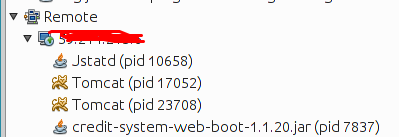
\includegraphics[scale=0.7]{visualvmconnectremote.png}
	\caption{VisualVM远程监控}
	\label{fig:visualvmconnectremote}
\end{figure}

目前可以通过VisualVM远程监控实现查看远程应用的PID、查看远程应用的启动参数、所使用的配置文件、JVM的版本以及路径、GC信息等等。Java的对象分为年轻代(Young Generation)和老年代(Old Generation)。年轻代又分为Eden(伊甸园)区和Survivor Space(幸存者),年老代是Tenured。当JVM无法在Eden区创建新对象时,则会出现Out of memory错误。使用JVM监控系统如图\ref{fig:monitorsystemmemory}所示:


\begin{figure}[htbp]
	\centering
	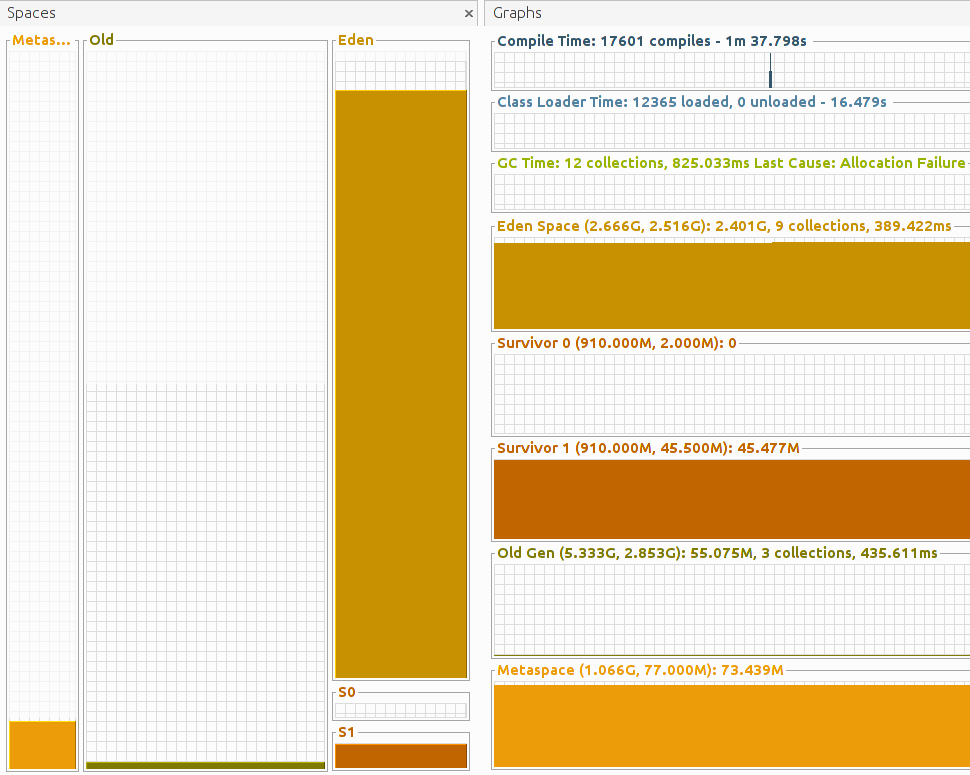
\includegraphics[scale=0.3]{monitorsystemmemory.png}
	\caption{VisualVM远程监控GC}
	\label{fig:monitorsystemmemory}
\end{figure}


\subsection{autojump}

autojump可以让你一键跳转到目标目录,一般情况下,很难准确的记忆清楚目标目录的准确路径,特别是目录嵌套比较深的时候。不停的重复使用cd命令一级或多级跳转显得有点笨拙。此时就可以使用autojump命令,只需要输入路径的关键字即可,比如只记得路径中隐约包含有关键字“jiangxiaoqiang”,那么仅仅输入命令autojump jiang,就可以自动跳转到对应的路径下。安装autojump:

\begin{lstlisting}[language=Bash]
sudo apt-get install autojump -y
# 给autojump命令设置别名
alias j='autojump'
# 从源代码安装autojump
git clone git://github.com/joelthelion/autojump.git
chmod 755 install.py
./install.py

# 将当前路径添加到autojump的搜索库
autojump -a 'pwd'
\end{lstlisting}

为了进一步简化目录跳转命令,可以直接添加命令autojump的别名:

\begin{lstlisting}[language=Bash]
alias j='autojump'
\end{lstlisting}

有时会出现如下的提示:Please source the correct autojump file in your shell's startup file. For more information, please reinstall autojump and read the post installation instructions.为了暂时激活autojump应用,即直到你关闭当前会话或打开一个新的会话之前让autojump均有效,需要以常规用户身份运行下面的命令:

\begin{lstlisting}[language=Bash]
# 在Linux系统下
source /usr/share/autojump/autojump.sh on startup
# 在Mac OS X下
source ~/.autojump/etc/profile.d/autojump.sh
# 也可运行如下命令
[[ -s /Users/dolphin/.autojump/etc/profile.d/autojump.sh ]] && source /Users/dolphin/.autojump/etc/profile.d/autojump.sh
\end{lstlisting}

为了使得autojump在BASH shell中永久有效,需要运行下面的命令。

\begin{lstlisting}[language=Bash]
echo '. /usr/share/autojump/autojump.sh'>>~/.bashrc
# 在Mac OS X下
echo '. ~/.autojump/etc/profile.d/autojump.sh'>>~/.bashrc
\end{lstlisting}

\section{Graphviz}

\subsection{编译}

一个简单的图形示例:

\begin{lstlisting}
digraph G {
	node [peripheries=2 style=filled color="#eecc80"]
	edge [color="sienna" fontcolor="green"]
	"componentWillMount" -> "serviceComponent";
	"serviceComponent" -> "axios";
	"axios" -> "dishatch data to store"[label="XHR(GET/POST/PUT/DELETE)"] ;
	"dishatch data to store" -> "props get data";
}
\end{lstlisting}

\begin{lstlisting}[language=Bash]
dot -Tjpg -Gdpi=1024 maven-lifecycle.dot -o maven-lifecycle.jpg
\end{lstlisting}

\subsection{subgraph}



\section{MyBatis Generator}




\chapter{Git}

\section{基础}

\subsection{配置}

常用语句。

\begin{lstlisting}[language=Bash]
git config --global user.name "dolphin"
git config --global user.email "jiangtingqiang@gmail.com"
#增加远程库
git remote add company-internal http://xiaoqiang.jiang@gitlab.data.com/backend/system.git
#删除远程库
git remote rm company-
#修改远程库地址
git remote set-url origin http://gitlab.hualongdata.com/internal/work-record.git
#列出git配置
git config --list
\end{lstlisting}

克隆指定的分支:

\begin{lstlisting}[language=Bash]
git clone -b v1.3 <url>
\end{lstlisting}

\subsection{返回到指定版本}

查看提交历史:

\begin{lstlisting}[language=Bash]
git log --all --graph -12
\end{lstlisting}

回滚到指定版本:

\begin{lstlisting}[language=Bash]
git reset --hard e4177ea9061a9726efd42d289f73553409df793d
\end{lstlisting}

结果如图\ref{fig:filemodifyhistory}所示,即可看到由谁修改。

\begin{figure}[htbp]
	\centering
	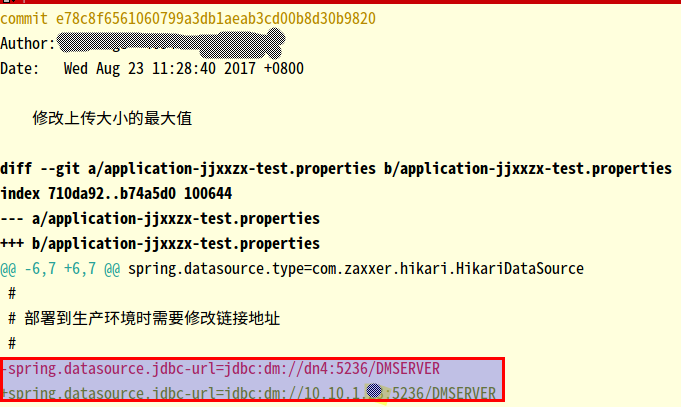
\includegraphics[scale=0.4]{filemodifyhistory.png}
	\caption{Git查看文件修改历史}
	\label{fig:filemodifyhistory}
\end{figure}

\subsection{标签(Tag)}

有的时候需要修复线上某个版本的问题,但是当前主分支已经合并了中途开发的部分功能,还未经过严格测试。为了满足这样的要求,需要在每次发布版本的时候打上标记(Tag),需要修复线上问题时,可以回到标记的版本,修复线上的问题后,将fix分支合并到主干。

\begin{lstlisting}[language=Bash]
# 发布时打上Tag,带有信息
git tag -a v1.1.31 -m "v1.0版本发布"
git tag -a v1.1.35 -m "v1.1.35-Release版本"
# 查看有哪些Tag
git tag
# 查看具体Tag的内容
git show v1.1.31
# 将代码回退到发布时的版本
# 实际Commit ID为
# eb8f7df1935da2e191163610d8b0374beff011e0
# 只需要前几位即可
git reset --hard eb8f7d
# 回退版本后,拉取新的分支,这里取名HotFix1.1.31分支
git checkout -b HotFix1.1.31
\end{lstlisting}

需要注意的是,创建好HotFix分支之后,要马上回到主分支将代码前进到最新版本:

\begin{lstlisting}[language=Bash]
# 切换到主分支
git checkout master
# 使用reflog命名检索最新版本的commit id
git reflog
# 前进到最新版本
git reset --hard 9e4c92
\end{lstlisting}

剩下的工作就是切换到刚才到HotFix1.1.31分支修复问题即可。修复之后,将问题修复后的代码合并到主干分支。

\subsection{log}

在项目中看到有几行代码,百思不得其解,也没有注释,所以想看一看作者,与作者沟通,使用如下命令即可:

\begin{lstlisting}[language=Bash]
git blame PubapiOrgController.java
\end{lstlisting}

会显示每一行代码的作者(最后修改者)和最后的修改时间。有的时候,不仅仅需要看某(几)行代码最后的修改,也希望看到最近几个版本的修改。比如有一次部署上去后,发现数据库链接被改掉了,那么可以使用如下命令查看文件的修改历史:

\begin{lstlisting}[language=Bash]
git log --follow application-jjxxzx-test.properties
\end{lstlisting}

会显示出指定文件的修改历史记录,使用如下命令查看详细的修改内容:

\begin{lstlisting}[language=Bash]
git show e78c8f6561060799a3db1aeab3cd00b8d30b9820
\end{lstlisting}

有时项目中的一个文件突然被删除了,需要查看具体是什么原因删除了文件,由谁删除的,可以使用如下命令:

\begin{lstlisting}[language=Bash]
git log -1 --stat -- 行政处罚模板.xlsx
git log -p -- 行政处罚模板.xlsx
\end{lstlisting}

如果当前路径不在删除文件路径下,需要写相对路径。stat表示statistic的意思,可以看一些统计信息,比如删除的文件个数等。

\subsection{merge}

配置Meld为默认合并工具:

\begin{lstlisting}[language=Bash]
git config --global merge.tool meld
\end{lstlisting}



\subsection{Cherry Pick}

项目开发有v1分支和v1.3分支,v1分支是旧版系统的分支,针对旧版系统的某些改造特性想在新版中集成,而其他的内容和问题修复不一定会集成到新版系统中。此时为了避免重复修改,可以使用git的cherry pick将指定的commit合并到新版分支中。使用如下命令:

\begin{lstlisting}[language=Bash]
git cherry-pick <commit id>
git cherry-pick e6abef4e
\end{lstlisting}

有时commit比较多,一个一个合并比较麻烦,Git从1.7.2版本开始支持批量cherry-pick,就是一次可以cherry-pick一个区间的commit,此时可以指定提交区间。

\begin{lstlisting}[language=Bash]
git cherry-pick <start-commit-id>..<end-commit-id>
git cherry-pick -x 472d65eb76..8f4ecc61f31828
\end{lstlisting}

error: Commit cb82fbb5a24211ba60f4826c5ceff25e31d397b9 is a merge but no -m option was given。cherry-pick合并时需要制定Parent Number。目前还没有搞清楚Parent Number如何查看,目前直接指定的1。

\begin{lstlisting}[language=Bash]
git log --pretty=format:"%P %H - %an, %ar : %s" --graph
\end{lstlisting}

\%H  提交对象(commit)的完整哈希字串
\%h  提交对象的简短哈希字串
\%T  树对象(tree)的完整哈希字串
\%t  树对象的简短哈希字串
\%P  父对象(parent)的完整哈希字串
\%p  父对象的简短哈希字串
\%an 作者(author)的名字
\%ae 作者的电子邮件地址
\%ad 作者修订日期(可以用 -date= 选项定制格式)
\%ar 作者修订日期,按多久以前的方式显示
\%cn 提交者(committer)的名字
\%ce 提交者的电子邮件地址
\%cd 提交日期
\%cr 提交日期,按多久以前的方式显示

\subsection{Reflog}

第一次使用Cherry Pick时没有注意当前的分支,导致许多历史Commit消失了,此时可以使用reflog命令,还好重新clone时没有删除原来的仓库。Reference logs, or "reflogs", record when the tips of branches and other references were updated in the local repository. Reflogs are useful in various Git commands, to specify the old value of a reference.每一次当前HEAD发生改变(包括切换branch, pull, 添加新commit)一个新的纪录就会被添加到reflog。使用如下命令查看所有Commit:

\begin{lstlisting}[language=Bash]
git reflog
\end{lstlisting}

结果如图\ref{fig:gitreflogfindcommit}所示:

\begin{figure}[htbp]
	\centering
	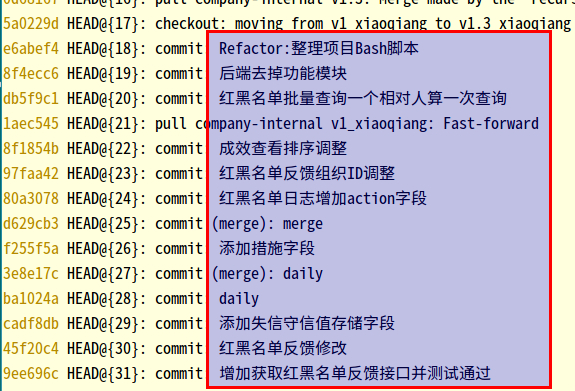
\includegraphics[scale=0.4]{gitreflogfindcommit.png}
	\caption{Git查看所有Commit}
	\label{fig:gitreflogfindcommit}
\end{figure}

将当前分支reset到指定的<commit>或者HEAD:

\begin{lstlisting}[language=Bash]
git reset --hard e6abef4
\end{lstlisting}

\subsection{常见问题}


\paragraph{error setting certificate verify location}

当你通过HTTPS访问Git远程仓库,如果服务器的SSL证书未经过第三方机构签署,那么Git就会报错。这是十分合理的设计,毕竟未知的没有签署过的证书意味着很大安全风险。但是,如果你正好在架设Git服务器,而正式的SSL证书没有签发下来,你为了赶时间生成了自签署的临时证书。

\begin{lstlisting}[language=Bash]
env GIT_SSL_NO_VERIFY=true git clone https://<host_name/git/project.git
\end{lstlisting}

或者将Git设置为不允许ssl认证:

\begin{lstlisting}[language=Bash]
git config --system http.sslverify false
\end{lstlisting}



\chapter{Google Chrome}

\section{DevTools}

\begin{tabular}{|c|p{6cm}|}
	\hline
	\multirow{1}{*}{快捷键}
	& \multicolumn{1}{c|}{备注}\\			
	\hline
	Ctrl+Shift+J (Windows/Linux)  & 打开DevTools Console面板 \\
	\hline
	Ctrl+Shift+I (Windows/Linux)  & 打开DevTools Network面板,I是Inspect的缩写 \\
	\hline
	Ctrl+Shift+P (Windows/Linux)  & 打开所有窗口 \\
	\hline
\end{tabular}

\subsection{Console}

\paragraph{Log XMLHttpRequests}

想要看到使用中应用发送的 XHR 请求,可以打开 settings 面板(译注:打开调试面板按 F1 呼出)选中 “Log XMLHttpRequests” 选项,然后就可以在 “Console” 面板中看到请求了。点击此请求可以导航到Network选项卡上,当然也可以直接在Network选项卡中查看XHR HttpRequest请求,不过使用Console打印出来到导航还是要方便一些,多了一个入口。

\paragraph{脚本添加到黑盒}

当你使用 “Event listener breakpoint :: Mouse :: Click” 调试事件时,有很大的可能是代码在第三方的库中中断了(例如 jquery ),这时如果你想找到属于自己项目的调用需要在调试器里面点很多次的下一步才能看到。 一种很棒的方式就是把这些第三方的脚本放到黑盒里面,调试器永远不会在黑盒中的脚本内停止,它会一直向后运行,直到运行的代码行位于黑盒之外的文件。 你可以在调用栈面板中右键点击第三方脚本的文件名,然后左键在下拉菜单中点击 “Blackbox Script”。

\paragraph{定位按钮触发代码}

快速定位某个特定按钮或者链接点击后所触发的代码,只需要在你真正点击按钮之前,激活一个 “Event listener breakpoint”, 选中右侧面板下 mouse 下面的 click 确认框即可。

\paragraph{Async调试}

在Promise被广泛应用的今天,我们都知道,Promise的回调是异步执行的,没有开启Async模式前,调动栈只记录到回调函数本身,我们无法找到代码执行的顺序,这给我们调试带来巨大的困难。Async模式可以解决这个问题。

\begin{figure}[htbp]
	\centering
	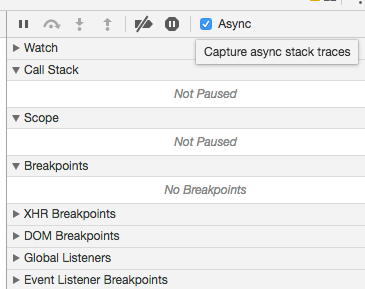
\includegraphics[scale=0.6]{chromeasyncdebugging.png}
	\caption{Google Chrome异步调试}
	\label{fig:chromeasyncdebugging}
\end{figure}

\paragraph{查找成员函数}

Ctrl+Shif+O文件中定位成员函数。

\paragraph{打印对象数组}

在Javascript中可能返回有数组,有的时候可能某一个数组元素感觉数据不对,在Javascript调试跟踪时,输出了一些Object对象,如果是几个元素,还可以一个一个点开查看,如果有成百上千的元素,一个一个点开查看几乎是不可能的,至今没有发现在结果中按关键字搜索的功能,此时可以使用如下方法:

\begin{lstlisting}[language=Bash]
console.table(data);
\end{lstlisting}

即可以表格的形式显示所有元素,其中data表示一个对象或者数组,如图\ref{fig:googlechromeconsoletable}所示。

\begin{figure}[htbp]
	\centering
	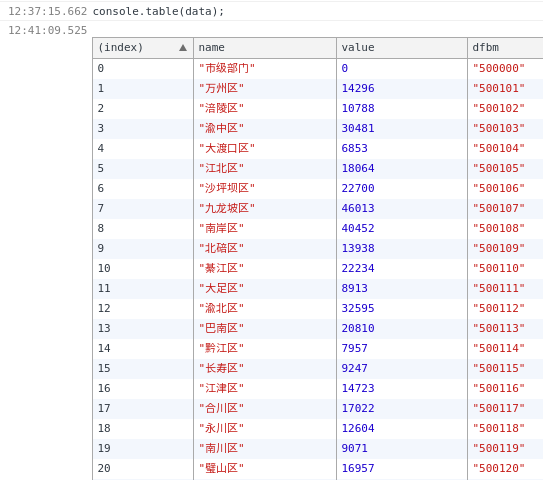
\includegraphics[scale=0.5]{googlechromeconsoletable.png}
	\caption{Google Chrome查看对象数组}
	\label{fig:googlechromeconsoletable}
\end{figure}


\subsection{Source Map}

截止目前几乎没有浏览器完全原生支持es6标准,对于这种情况,Chrome引入了source-map文件,标识es5代码对应的转码前的es6代码哪一行,唯一要做的就是配置webpack自动生成source-map文件,这也很简单,在webpack.config.js中增加一行配置即可(需要重新启动webpack-dev-server使配置生效)


\subsection{Network}

\paragraph{Replay XHR}

有时在开发时,可以直接在Network中的网络请求列表中点击右键,在菜单中重复发送XHR请求(Replay XHR),不需要再次进入界面模拟请求,可以提高不少效率。

\paragraph{Disable cache}

勾选上Disable cache后,浏览器不会利用本地的Javascript缓存,每次都会到服务器上重新取。

\paragraph{Preserve Log}

保留请求日志,勾选后,即使在当前页面刷新后,日志也不会清空。在使用large request row后,size和time会出现2行内容,如图\ref{fig:networksizeandtime}所示。其中时间行,上面的时间代表从请求开始到接收完最后一个byte为止的时间,下面一行是Latency,代表从请求接收完后到读取该资源第一个byte之间的等待时间。按照这个逻辑,那么上面一行的时间减去下面一行的时间就是数据的下载时间,将鼠标移动到右侧waterfall图标上,可以看到下载时间(Content Download)正好是上下两行的时间差。另外Size列也有2行,上面一行代表网络上实际传输的文件大小,下面一行代表原始的未经过压缩的文件大小。一般服务器会对资源使用Gzip进行压缩。

\begin{figure}[htbp]
	\centering
	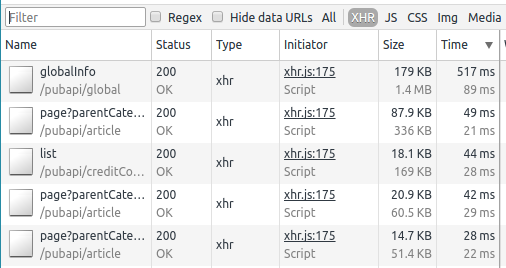
\includegraphics[scale=0.6]{networksizeandtime.png}
	\caption{Network宽行显示}
	\label{fig:networksizeandtime}
\end{figure}

\paragraph{DOMContentLoaded和load事件信息}

DOMContentLoaded和load这两个事件会高亮显示。DOMContentLoaded事件会在页面上DOM完全加载并解析完毕之后触发,不会等待CSS、图片、子框架加载完成。load事件会在页面上所有DOM、CSS、JS、图片完全加载完毕之后触发。DOMContentLoaded事件在Overview上用一条蓝色竖线标记,并且在Summary以蓝色文字显示确切的时间。load事件同样会在Overview和Requests Table上用一条红色竖线标记,在Summary也会以红色文字显示确切的时间。

\paragraph{资源的发起者(请求源)和依赖项}

通过按住Shift并且把光标移到资源名称上,可以查看该资源是由哪个对象或进程发起的(请求源)和对该资源的请求过程中引发了哪些资源(依赖资源)。在该资源的上方第一个标记为绿色的资源就是该资源的发起者(请求源),有可能会有第二个标记为绿色的资源是该资源的发起者的发起者,以此类推。在该资源的下方标记为红色的资源是该资源的依赖资源,如图\ref{fig:resourcedependency}所示。

\begin{figure}[htbp]
	\centering
	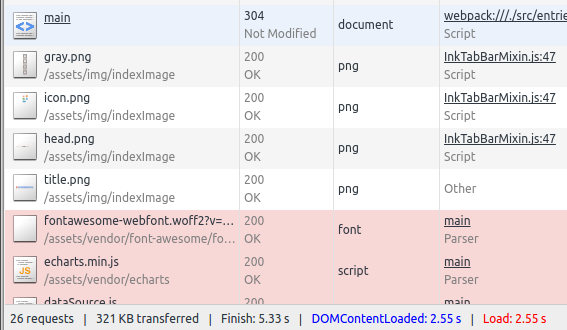
\includegraphics[scale=0.5]{resourcedependency.png}
	\caption{依赖资源}
	\label{fig:resourcedependency}
\end{figure}


\subsection{Elements}

在元素上,按住Ctrl + Alt + 鼠标左键,可以展开元素及下级元素的所有节点。


\subsection{Performance}



\subsection{Sources}

\paragraph{面板中查看变量}

在调试的过程中,虽然鼠标可以移动到变量上会自动Pop出对应的变量,但是有时候鼠标移出区域后变量也会自动消失。那么此时可以在右侧面板中的Scope查看变量,如图\ref{fig:sourcepanelscopevariable}所示:

\begin{figure}[htbp]
	\centering
	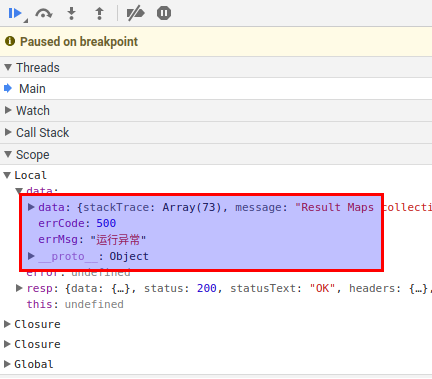
\includegraphics[scale=0.4]{sourcepanelscopevariable.png}
	\caption{Devtool Scope中查看变量}
	\label{fig:sourcepanelscopevariable}
\end{figure}




\subparagraph{查看Render区域}

有时需要查看浏览器重绘制的区域,页面的绘制时间(paint time)是每一个前端开发都需要关注的的重要指标,它决定了你的页面流畅程度。使用Ctrl + Shift + P,输入Render打开对应页面即可。而如何去观察页面的绘制时间,找到性能瓶颈,可以借助Chrome的开发者工具,激活页面绘制区域显示如图\ref{fig:pagepainting}所示。

\begin{figure}[htbp]
	\centering
	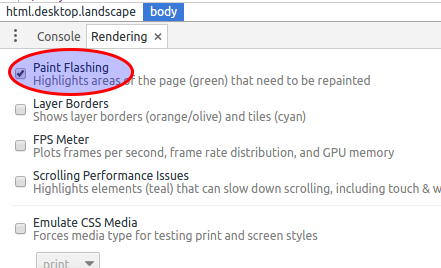
\includegraphics[scale=0.6]{pagepainting.png}
	\caption{激活页面绘制区域高亮}
	\label{fig:pagepainting}
\end{figure}

\subsection{Audits}

\subsection{Google Chrome SSH}

\chapter{LaTex}

\section{安装}

输入如下命令安装TexLive:

\begin{lstlisting}[language=Bash]
# Ubuntu下安装Texlive
sudo apt-get install texlive -y
\end{lstlisting}

\subsection{字体}

Computer Modern是自由软件TeX的默认字体,为美国计算机科学家高德纳(Donald Knuth)使用METAFONT软件创造。但是此字体不是很漂亮,所以考虑换一个字体 。

\paragraph{lstlisting字体}

在使用lstlisting代码块时,希望使用等宽字体(Monospaced Font),代码使用等宽字体更加美观。lstlisting设置如下:

\begin{lstlisting}[language=Tex]
\lstset{
	% 设定代码的基本字体为等宽字体(类似于Courier)
	basicstyle=\ttfamily,
	% 设定注释部分字体为等宽字体,用深绿色显示    
	commentstyle=\ttfamily\color{green!40!black},    
}
\end{lstlisting}


\subsection{版面}

\paragraph{PDF导航深度}

\LaTeX{}生成的pdf导航默认深度是3,如果需要显示更深层次。那么可以使用hyperref包,如下代码片段。

\begin{lstlisting}[language=Tex]
\usepackage[bookmarksopen,bookmarksdepth=3]{hyperref}
\end{lstlisting}

奇怪的是,这种方式在Mac OS X下有效,但是在Ubuntu 16.04LTS下无效。

\paragraph{换行}Latex的自动拆单词换行是依靠字典的。如果遇到\LaTeX{}不认识的单词,他就不会换行了。后面的内容就会溢出。

\subsection{支持语言}

Latex原生不支持JavaScript语言,添加如下定义:

\begin{lstlisting}[language=Tex]
%lstlisting包JavaScript语言设置
\lstdefinelanguage{JavaScript}{
	keywords={typeof, new, true, false, catch, function, return, null, catch, switch, var, if, in, while, do, else, case, break},
	keywordstyle=\color{blue}\bfseries,
	ndkeywords={class, export, boolean, throw, implements, import, this},
	ndkeywordstyle=\color{darkgray}\bfseries,
	identifierstyle=\color{black},
	sensitive=false,
	comment=[l]{//},
	morecomment=[s]{/*}{*/},
	commentstyle=\color{purple}\ttfamily,
	stringstyle=\color{red}\ttfamily,
	morestring=[b]',
	morestring=[b]"
}
\end{lstlisting}

即可在文档中定义JavaScript,并支持关键字颜色区分。

\subsection{常见问题}

\paragraph{infoBulle.sty not found}

一般的,.cls和.sty文件是用来提高LaTeX的排版效果的补充文件。它们分别用命令\textbackslash documentclass\{...\}和命令\textbackslash usepackage\{...\}来装载到LaTeX文件。.cls文件通常被称为“classes”(也就是“类”),而.sty文件被称为“style files”(样式文件),或者就简单地称其为“packages”(包)。

下载下来的宏包,有的直接包含.sty 文件(.sty文件就是package的最终形式);有的下载下来只包含了.ins, .dtx,以及一个readme文件,这时需要自己编译生成.sty文件,以及生成相应的manual。
,你可以在这个路径下建立一个文件夹,譬如qrcode,然后把qrcode.sty放到这里,接着在你的电脑里找到MikTex的settings这个程序,settings有两个,选择后面括号里有admin的那个,打开以后,在general选项卡下有Refresh FNDB按钮,点击,过一会,这个package就会加入MikTex的路径中,然后在你的tex文件中就可以使用这个package了。

infoBulle可能是作者自己写的一个宏包,系统里默认没有自带,此时就需要找到默认宏包的存放目录,将作者自己写的sty文件放进去。在Mac OS X下,路径为:

\begin{lstlisting}
/usr/local/texlive/2016/texmf-dist/tex/latex
\end{lstlisting}

sty文件拷贝到指定目录后,运行命令:

\begin{lstlisting}[language=Bash]
sudo texhash
\end{lstlisting}

即可使用命令引用包。有时会提示缺少sty文件,遇到一次是因为没有完全安装latex,输入完整包安装命令:

\begin{lstlisting}[language=Bash]
sudo apt-get install texlive-full -y
\end{lstlisting}

\paragraph{中文支持}

在Ubuntu 14.04 LTS下编译无法显示中文,在\LaTeX{}中指定中文字体即可:

\begin{lstlisting}[language=Tex]
% 设置缺省中文字体
\setCJKmainfont{WenQuanYi Micro Hei} 
\end{lstlisting}

\part{DB}

\chapter{性能(Performance)}

\section{索引(Index)}

\subsection{索引常识}

绝大多数情况下,数据库只使用一个索引。在开发中遇到有时根据时间查询很快:

\begin{lstlisting}[language=SQL]
--在列org\_id和jdrq上都建立了索引
--同样都查询语句,不同都org\_id值会有不同都查询性能
--当org\_id结果集很少当时候,数据库会使用org\_id索引
--在使用了org\_id索引后,不会使用jdrq索引
--同理,当org\_id结果集更大,根据jdrq索引效率更高时
--数据库会使用jdrq列作为索引,而不会使用org\_id索引
select *
from table
where org_id = '1000'
order by jdrq desc
\end{lstlisting}

所以需要同时利用多个列的索引,或者查询条件包含多列时,应该使用联合索引。

\begin{lstlisting}[language=SQL]
create index idx_ts_b_xzxk_jdrq_org_id on xzxk(jdrq desc,org_id);
\end{lstlisting}

\paragraph{B+树}

IO次数取决于b+数的高度h(height),假设当前数据表的数据为N,每个磁盘块的数据项的数量是m,则有

\begin{equation}
h=\log_{(m+1)} N
\end{equation}


当数据量N一定的情况下,m越大,h越小;而m = 磁盘块的大小 / 数据项的大小,磁盘块的大小也就是一个数据页的大小,是固定的,如果数据项占的空间越小,数据项的数量越多,树的高度越低。这就是为什么每个数据项,即索引字段要尽量的小,比如int占4字节,要比bigint8字节少一半。这也是为什么b+树要求把真实的数据放到叶子节点而不是内层节点,一旦放到内层节点,磁盘块的数据项会大幅度下降,导致树增高。当数据项等于1时将会退化成线性表。

当b+树的数据项是复合的数据结构,比如(name,age,sex)的时候,b+数是按照从左到右的顺序来建立搜索树的,比如当(张三,20,F)这样的数据来检索的时候,b+树会优先比较name来确定下一步的所搜方向,如果name相同再依次比较age和sex,最后得到检索的数据;但当(20,F)这样的没有name的数据来的时候,b+树就不知道下一步该查哪个节点,因为建立搜索树的时候name就是第一个比较因子,必须要先根据name来搜索才能知道下一步去哪里查询。比如当(张三,F)这样的数据来检索时,b+树可以用name来指定搜索方向,但下一个字段age的缺失,所以只能把名字等于张三的数据都找到,然后再匹配性别是F的数据了, 这个是非常重要的性质,即索引的最左匹配特性\footnote{\url{参考链接:http://tech.meituan.com/mysql-index.html}}。

\paragraph{索引原则(Index Principle)}

\subparagraph{最左前缀匹配原则}

最左前缀匹配原则,非常重要的原则,mysql会一直向右匹配直到遇到范围查询(>、<、between、like)就停止匹配,比如a = 1 and b = 2 and c > 3 and d = 4 如果建立(a,b,c,d)顺序的索引,d是用不到索引的,如果建立(a,b,d,c)的索引则都可以用到,a,b,d的顺序可以任意调整。组合索引的第一个字段必须出现在查询组句中,这个索引才会被用到。举个例子:

\begin{lstlisting}[language=SQL]
select * 
from DOLPHIN  
where DFBM = '500101'  
order by JDRQ DESC 
limit 0, 10
\end{lstlisting}

在建立索引时,DFBM列一定要排在前面,建立(DFBM,JDRQ)这样的索引DB才会利用索引。如果顺序不对(JDRQ,DFBM),那么DB将不会采用索引。在mysql中执行查询时,只能使用一个索引,如果我们在lname,fname,age上分别建索引,执行查询时,只能使用一个索引,mysql会选择一个最严格(获得结果集记录数最少)的索引。

\subparagraph{=和in可以乱序}=和in可以乱序,比如a = 1 and b = 2 and c = 3 建立(a,b,c)索引可以任意顺序,mysql的查询优化器会帮你优化成索引可以识别的形式

\subparagraph{尽量选择区分度高的列作为索引}尽量选择区分度高的列作为索引,区分度的公式是count(distinct col)/count(*),表示字段不重复的比例,比例越大我们扫描的记录数越少,唯一键的区分度是1,而一些状态、性别字段可能在大数据面前区分度就是0,那可能有人会问,这个比例有什么经验值吗?使用场景不同,这个值也很难确定,一般需要join的字段我们都要求是0.1以上,即平均1条扫描10条记录

\subparagraph{索引列不能参与计算}索引列不能参与计算,保持列“干净”,比如from\_unixtime(create\_time) = ’2014-05-29’就不能使用到索引,原因很简单,b+树中存的都是数据表中的字段值,但进行检索时,需要把所有元素都应用函数才能比较,显然成本太大。所以语句应该写成create\_time = unix\_timestamp(’2014-05-29’);

\subparagraph{尽量的扩展索引}尽量的扩展索引,不要新建索引。比如表中已经有a的索引,现在要加(a,b)的索引,那么只需要修改原来的索引即可

\subsection{索引类型}

\subparagraph{位图索引(Bitmap Index)}

相对于B*Tree索引,占用的空间非常小,创建和使用非常快。位图索引由于只存储键值的起止Rowid和位图,占用的空间非常少。B*Tree索引由于不记录空值,当基于is null的查询时,会使用全表扫描,而对位图索引列进行is null查询时,则可以使用索引。当select count(XX) 时,可以直接访问索引中一个位图就快速得出统计数据。当根据键值做and,or或 in(x,y,..)查询时,直接用索引的位图进行或运算,快速得出结果行数据。

\subparagraph{散列索引Or哈希索引(Hash Index)}

散列索引是根据HASH算法来构建的索引,所以检索速度很快,但不能范围查询。散列索引的特点,只适合等值查询(包括= <> 和in),不适合模糊或范围查询

\subparagraph{聚集索引(Cluster Index)}

聚集索引确定表中数据的物理顺序。聚集索引类似于电话簿,后者按姓氏排列数据。由于聚集索引规定数据在表中的物理存储顺序,因此一个表只能包含一个聚集索引。但该索引可以包含多个列(组合索引),就像电话簿按姓氏和名字进行组织一样。 

\subparagraph{非聚集索引(Non-Cluster Index)}

它并不决定数据在磁盘上的物理排序,索引上只包含被建立索引的数据,以及一个行定位符row-locator,这个行定位符,可以理解为一个聚集索引物理排序的指针,通过这个指针,可以找到行数据。

\subparagraph{全文索引(Full-text Search)}

全文索引是基于要编制索引的文本中的各个标记来生成倒排序、堆积且压缩的索引结构。每个表或索引视图只允许有一个全文索引。该索引最多可包含 1024 列。,该对象中必须有一唯一并且非空的列。 

\subparagraph{联合索引}

联合索引能够满足最左侧查询需求,例如(a, b, c)三列的联合索引,能够加速a | (a, b) | (a, b, c) 三组查询需求。这也就是为何不建立(passwd, loginName)这样联合索引的原因,业务上几乎没有passwd的单条件查询需求,而有很多loginName的单条件查询需求。

\subsection{like查询优化}

目前数据量将近千万,模糊查询效率比较低。模糊查询通常有下面三种,前匹配:like \%abc,可以使用btree索引优化,后匹配:like abc\%,可以使用reverse函数btree索引,全匹配:like \%abc\%,可以使用pg\_trgm的gin索引。后面的2种优化方式是在PostgreSQL数据库中。还有全文索引技术也可以用来优化基于like查询的匹配。

\paragraph{采用函数(无效)}

采用函数来优化查询(没有效果):

\begin{lstlisting}[language=SQL]
--120W数据平均2.3秒左右,比原生查询稍慢
SELECT `column` FROM `table` WHERE LOCATE('keyword', `field`)>0

select * 
from "table" 
where locate('陶然居',mc)>0
and code is not null
limit 0,10;

--120W数据平均1.8秒左右,与原生查询时间相仿
SELECT `column` FROM `table` WHERE POSITION('keyword' IN `filed`)

select * 
from "table" 
where position('西南铝业' in mc)
and code is not null
limit 0,10;

--120W数据平均1.8秒左右,与原生查询时间相仿
SELECT `column` FROM `table` WHERE INSTR(`field`, 'keyword' )>0

select * 
from "table" 
where INSTR('西南铝业' in mc)>0
and code is not null
limit 0,10;
\end{lstlisting}

\paragraph{全文索引(Full-text Search)}

当使用like进行模糊搜索时,如果是中间匹配,那么无法使用索引,需要全表扫描(Full Table Scan)。优化?没有办法优化,所以不要花费时间在通过优化SQL语句来提升like中间匹配的查询效率。此时需要使用全文索引,一种方案是使用全文索引查询出结果后,再使用like进行匹配,在达梦数据库中创建全文索引:

\begin{lstlisting}[language=SQL]
create context index qymcindex on TS_F_CORPORATION(qymc) lexer CHINESE_VGRAM_LEXER;
alter context index qymcindex on TS_F_CORPORATION rebuild;
create context index xzcffulltextindex on TS_B_XZCF(xdr) lexer CHINESE_VGRAM_LEXER;
alter context index xzcffulltextindex on TS_B_XZCF rebuild;
\end{lstlisting}

填充索引:

\begin{lstlisting}[language=SQL]
alter context index qymcindex1 on user_xycq.TS_F_CORPORATION rebuild;
\end{lstlisting}

删除索引:

\begin{lstlisting}[language=SQL]
drop context index qymcindex on user_xycq.TS_F_CORPORATION_TEST;
\end{lstlisting}

达梦数据库中,在写全文索引查询时,全文索引的条件需要放到前面,这样才能够利用到索引。

\section{Redis}

\subsection{安装}

这里是在Raspberry Pi上安装Redis:

\begin{lstlisting}[language=Bash]
# 下载源码
wget -c http://download.redis.io/releases/redis-3.2.9.tar.gz
# 编译安装
make
make test
\end{lstlisting}

\chapter{PostgreSQL}

PostgreSQL是自由的对象-关系型数据库服务器(数据库管理系统),在灵活的BSD-风格许可证下发行。它在其他开放源代码数据库系统(比如MySQL和Firebird),和专有系统比如Oracle、Sybase、IBM的DB2和Microsoft SQL Server之外,为用户又提供了一种选择。

\section{基础操作}

\subsection{安装(Install)}

由于OS发行版本特殊,没有现成Binary包,所以从源码手动编译安装,选择的是9.6.5版本,运行configure的时候出现如下错误:

configure: error: readline library not found
If you have readline already installed, see config.log for details on the
failure.  It is possible the compiler isn't looking in the proper directory.
Use --without-readline to disable readline support.

提示缺失readline\footnote{\url{https://cnswww.cns.cwru.edu/php/chet/readline/rltop.html}}包,GNU Readline 是一个开源的程序库,可以实现交互式的文本编辑功能。网上说安装readline-devel包和libtermcap-devel包可以解决这个问题\footnote{\url{http://www.thegeekstuff.com/2009/04/linux-postgresql-install-and-configure-from-source}}(Install the readline-devel and libtermcap-devel\footnote{\url{https://centos.pkgs.org/5/centos-x86_64/libtermcap-devel-2.0.8-46.1.x86_64.rpm.html}} to solve the above issue).

由于是内网,无法连接互联网,手动安装依赖太复杂(包的依赖复杂,A包依赖B包,B包依赖C包,安装几个包之后整个人都不好了,这才真的真的体会到包管理工具的方便)。所以考虑了2个方案,一是在内网搭建一个离线yum(Yellowdog Updater, Modified\footnote{\url{https://en.wikipedia.org/wiki/Yum_(.rpm)}})源服务器,二是在可以连接互联网的机器上采用yum下载好包之后,在另一台内网机器上手动安装。使用如下命令下载依赖包:

\begin{lstlisting}[language=Bash]
sudo yum install --downloadonly <package-name>
yum install --downloadonly -y perl-ExtUtils-Embed readline-devel zlib-devel pam-devel libxml2-devel libxslt-devel openldap-devel python-devel gcc-c++ openssl-devel cmake
# Ubuntu下仅仅下载而不安装软件包
# 下载的目录一般为/var/cache/apt/archives
sudo apt-get -d install wget
\end{lstlisting}

参数d表示仅仅在下载模式(Dowanload Mode),并不会安装软件,默认情况下,一个下载的RPM包会保存在下面的目录中:

\begin{lstlisting}[language=Bash]
/var/cache/yum/x86_64/[centos/fedora-version]/[repository]/packages 
\end{lstlisting}

如果想要将一个包下载到一个指定的目录(如/tmp):

\begin{lstlisting}[language=Bash]
sudo yum install --downloadonly --downloaddir=/tmp <package-name> 
\end{lstlisting}


登录:

\begin{lstlisting}[language=Bash]
sudo -u postgres psql
\end{lstlisting}

这里是以超级用户的身份登录,否则在修改密码时会提示:must be superuser to alter superusers。修改密码:

\begin{lstlisting}[language=Bash]
\password postgres
\end{lstlisting}

Gradle引用驱动:

\begin{lstlisting}[language=Bash]
compile "org.postgresql:postgresql:42.1.1"
\end{lstlisting}

PostgreSQL新建列时,列名推荐使用小写,列名使用小写时,select里大小写都可以查询,如果列名为大写,查询语句中列名需要添加双引号才能查询。

\chapter{MySQL}

\subsection{查询}

\paragraph{MySQL远程连接(MySQL Remote Connection)}

本来以为安装完毕MySQL就可以自动进行远程连接,结果竟然花了半天时间才搞定。安装完毕后MySQL默认是不能远程连接的,由于在其他主机上用nmap无法扫描到端口3306,开始还以为是防火墙的缘故,在错误的道路上研究了许久,最后竟然在本机也无法扫描到端口。才明白MySQL是与localhost绑定而不是与IP绑定。在目录/etc/mysql/目录中修改配置文件my.cnf:

\begin{lstlisting}[language=Bash]
# Instead of skip-networking the default is now to listen only on
# localhost which is more compatible and is not less secure.
bind-address            = 192.168.31.25
\end{lstlisting}

默认是127.0.0.1,是一个回环地址,只有本机请求本机,目标地址才会是127.0.0.1,此时需要在其他主机请求,需要将绑定IP改为网卡地址, 也就是外网IP, 因为远程连接数据库目标IP肯定是公网IP. 不过还可以改成0.0.0.0,这样就表示监听所有IP, 只要端口一样, 网卡都会把请求传给进程。如果不在配置文件中修改地址,则需要在启动时指定绑定地址:

\begin{lstlisting}[language=Bash]
sudo mysqld --bind-address=192.168.31.25
\end{lstlisting}

绑定好地址后,使用命令sudo lsof:3306查看。如果填写的绑定地址是192开头,那么最终只有192开头的局域网里的机器能够远程连接MySQL,有时一台设备可能会处于多个局域网中,那么此时另一个局域网的设备就无法远程连接MySQL了。此时可以将绑定地址修改为0.0.0.0,即允许所有的IP连接到MySQL,相应的MySQL的安全性相应的就降低了。

\subsection{Mac中MySQL初始密码}

step1:

苹果->系统偏好设置->最下边点mysql 在弹出页面中 关闭mysql服务(点击stop mysql server)

step2:

进入终端输入:cd /usr/local/mysql/bin/
回车后 登录管理员权限 sudo su
回车后输入以下命令来禁止mysql验证功能 ./mysqld\_safe --skip-grant-tables \&
回车后mysql会自动重启(偏好设置中mysql的状态会变成running)

step3. 
输入命令 ./mysql
回车后,输入命令 FLUSH PRIVILEGES; 
回车后,输入命令 SET PASSWORD FOR 'root'@'localhost' = PASSWORD('你的新密码');

\subsection{基础}

启动MySQL:

\begin{lstlisting}[language=Bash]
mysqld

# Mac中启动MySQL,同理停止的参数为stop,重启的参数为restart
sudo /usr/local/MySQL/support-files/mysql.server start

# 防火墙添加端口
sudo iptables -A INPUT -p tcp --dport 3306 -j ACCEPT /*允许包从3306端口进入*/
sudo iptables -A OUTPUT -p tcp --sport 3306 -m state --state ESTABLISHED -j ACCEPT /*允许从3306端口进入的包返回*/

# 查看iptables
sudo iptables --list
SHOW DATABASES                                //列出 MySQL Server 数据库。
SHOW TABLES [FROM db_name]                    //列出数据库数据表。
SHOW TABLE STATUS [FROM db_name]              //列出数据表及表状态信息。
SHOW COLUMNS FROM tbl_name [FROM db_name]     //列出资料表字段
SHOW FIELDS FROM tbl_name [FROM db_name],DESCRIBE tbl_name [col_name]。
SHOW FULL COLUMNS FROM tbl_name [FROM db_name]//列出字段及详情
SHOW FULL FIELDS FROM tbl_name [FROM db_name] //列出字段完整属性
SHOW INDEX FROM tbl_name [FROM db_name]       //列出表索引。
SHOW STATUS                                  //列出 DB Server 状态。
SHOW VARIABLES                               //列出 MySQL 系统环境变量。
SHOW PROCESSLIST                             //列出执行命令。
SHOW GRANTS FOR user                         //列出某用户权限
GRANT ALL PRIVILEGES ON *.* TO 'root'@'192.168.31.25'IDENTIFIED BY 'dolphin' WITH GRANT OPTION;
\end{lstlisting}

在使用MySQL会出现中文乱码问题,MySQL的字符集支持(Character Set Support)有两个方面:字符集(Character set)和排序方式(Collation)。对于字符集的支持细化到四个层次: 服务器(server),数据库(database),数据表(table)和连接(connection)。在Mac中,在etc目录下新建my.cnf文件,指定数据库编码:

\begin{lstlisting}[language=Bash]
[mysqld]
character-set-server=utf8
init_connect='SET NAMES utf8'
[mysql]
default-character-set=utf8
\end{lstlisting}

修改后,重新启动数据库。但是以前新建的表有可能还是采用的原来的编码,使用如下语句进行修改:

\begin{lstlisting}[language=SQL]
--检查数据表所有字段的状态	
show full columns from book; 
--发现address字段的Collation项非utf8,改成utf8
alter table book change publisher publisher varchar(512) character set utf8 collate utf8_unicode_ci not null;
\end{lstlisting}

\subsection{备份}

netstat -ln | grep mysql

mysqldump --sock=/var/run/mysqld/mysqld.sock -u root -p dolphin>dolphin.sql

\subsection{存储过程}

\begin{lstlisting}[language=SQL]
DELIMITER $$

CREATE DEFINER=`root`@`%` PROCEDURE `insert_initial_id`()
BEGIN  

DECLARE i INT DEFAULT 1;# can not be 0  
DECLARE j INT DEFAULT 10000000;# can not be 0  


WHILE i<99999999 && j < 10000050
DO  
insert into douban_book_id(isscapy,douban_book_id) values (0,j);  
SET i=i+1;  
set j=j+1;
END WHILE ;  
commit;  

END$$
DELIMITER ;
\end{lstlisting}


\subsection{mycli}

MyCli 是一个 MySQL 命令行工具,支持自动补全和语法高亮。也可用于 MariaDB 和 Percona。安装mycli:

\begin{lstlisting}[language=Bash]
pip install mycli
brew install mycli
\end{lstlisting}

使用MyCli连接数据库示例如下:

\begin{lstlisting}[language=Bash]
mycli -h 10.0.0.14 -u root -p dolphin
\end{lstlisting}

在Ubuntu下远程配置如图\label{raspberryremtoeconfig}所示:

\subsection{常见问题}

\paragraph{ERROR 2002 (HY000): Can't connect to local MySQL server through socket '/tmp/mysql.sock'}

mysql使用unix socket或者tcp来连接数据库进行通讯,默认不加 -h选项时使用的就是localhost即unixsocket,此时会通过/tmp/mysql.sock来通讯,但是在配置文件中默认生成的socket文件是在/var/lib/mysql/mysql.sock(不同安装可能不同,建议查看/etc/my.cnf确认),所以要想mysql使用这个文件通讯,最简单的方法就是建立软链接,一劳永逸,此为方法一

方法二就是强制mysql使用tcp通讯,因为127.0.0.1对于mysql来说走的是tcp协议而非unixsocket,这种方法的弊端就是每次都要指明本地地址127.0.0.1

\subsection{中文查询}

在用MyBatis查询中文时,出来的结果却不是中文匹配的结果,将SQL在客户端工具中执行却可以正确查询。在MySQL配置文件中修改相应的编码。在服务端/etc/mysql/my.cnf修改相应编码:

\begin{lstlisting}[language=Bash]
[mysqld]

character-set-server=utf8
\end{lstlisting}




\chapter{达梦}

启动达梦:

\begin{lstlisting}[language=Bash]
/home/hldev/dmdbms/bin/dmserver /home/hldev/dmdbms/data/DAMENG/dm.ini -noconsole
\end{lstlisting}




\section{SQL}

\subsection{索引}

全文索引未生效时,可以到CTISYS模式下查看系统所有的全文索引:

\begin{lstlisting}[language=SQL]
select * 
from "CTISYS"."SYSCONTEXTINDEXES";
\end{lstlisting}

新建索引时,选择独立的索引存储空间,最好是索引存储与数据存储独立,便于管理。每个用户建立一个数据表空间,一个索引表空间。采用函数的列应该保存在索引中。添加上(a,b,c)的组合索引相当于添加了,超过3个列的联合索引不合适,否则虽然减少了回表动作,但索引块过多,查询时就要遍历更多的索引块了,建索引动作应谨慎,因为建索引的过程会产生锁,不是行级锁,而是锁住整个表,任何该表的DML操作都将被阻止,在生产环境中的繁忙时段建索引是一件非常危险的事情。

在达梦客户端中,按下Ctrl + Alt + L会出来所有快捷键的面板,不得不说这个设计还是非常贴心的,开始真的不敢相信自己的眼睛,反复确认了真的不是Intellij Idea调出的面板,是达梦调出来的,非常不错的设计。注意平台是Ubuntu 16.04 LTS。

\subsection{函数}

根据条件来计算:

\begin{lstlisting}[language=SQL]
SELECT ORG_ID,
ORG_NAME,
INTERFACE_NAME,
COUNT(*) AS TOTAL,
SUM(CASE WHEN RETURN_COUNT > 0 THEN 1 ELSE 0 END) AS VALID_TIMES,
ROUND(CONVERT(DOUBLE,SUM(CASE WHEN RETURN_COUNT > 0 THEN 1 ELSE 0 END))/CONVERT(DOUBLE,COUNT(*)),3) AS RATIO
FROM TD_M_APPACCESS_LOG
GROUP BY ORG_ID,ORG_NAME,INTERFACE_NAME
\end{lstlisting}

如上语句统计接口的有效调用次数,返回数量(RETURN\_COUNT)大于0时,视为有效调用次数(VALID\_TIMES)。数量默认为整数,所以要得到小数的比率(RATIO),就需要使用函数convert将数据转换为Double类型。

\subsection{常用SQL记录}

嵌套查询:

\begin{lstlisting}[language=SQL]
select GNMK,
max(ORG_NAME) as ORG_NAME,
ORG_ID,
COUNT(*) AS USING_TIMES,
SUM(CASE WHEN ISOKRED > 0 OR ISBLACKRED > 0 THEN 1 ELSE 0 END) AS VALID_TIMES,
SUM(CASE WHEN ISOKRED > 0 THEN 1 ELSE 0 END) AS VALID_COUNT_RED,
SUM(CASE WHEN ISBLACKRED > 0 THEN 1 ELSE 0 END) AS VALID_COUNT_BLACK
from (
	SELECT GNMK,
	MAX(ORG_NAME) AS ORG_NAME,
	ORG_ID,
	sum(ISOKRED) as ISOKRED,
	sum(ISOKBALCK) AS ISBLACKRED,
	RESPONSEKEY	
	FROM TI_B_REDBALCKLOG  
	GROUP BY RESPONSEKEY,ORG_ID,GNMK 
)
GROUP BY ORG_ID,GNMK 
order by ORG_ID DESC limit 0, 10

--修改参数
select * 
from v$dm_ini
where para_name like '%ORDER%'

select * from v$sessions where state='ACTIVE';
\end{lstlisting}

删除数据库ID重复的记录,只保留其中一条记录:

\begin{lstlisting}[language=SQL]
delete from dolphin where rowid not in(select max(rowid) from dolphin group by id) 
\end{lstlisting}

拼接列:




\section{通用知识}

\subsection{查询优化}

最近使用数据库中,遇到查询性能低下的问题。数据量大概在800W左右,但是分页查询需要40s左右才能够查询出来结果,测试库200W数据量左右,分页查询也需要10s才能出结果。

使用MySQL,有的人BB说5.1以前300w就会很明显,5.5-5.6已经有很大优化,如果是5.7千万也不是问题。随着互联网的发展,数据的量级也是撑指数的增长,从GB到TB到PB。对数据的各种操作也是愈加的困难,传统的关系性数据库已经无法满足快速查询与插入数据的需求。这个时候NoSQL的出现暂时解决了这一危机。它通过降低数据的安全性,减少对事务的支持,减少对复杂查询的支持,来获取性能上的提升。但是,在有些场合NoSQL一些折衷是无法满足使用场景的,就比如有些使用场景是绝对要有事务与安全指标的。这个时候NoSQL肯定是无法满足的,所以还是需要使用关系性数据库。

\paragraph{增加缓存}增加缓存可以提高查询效率,但是在对数据表做任何的更新操作(update/insert/delete)等操作,server为了保证缓存与数据库的一致性,会强制刷新缓存数据,导致缓存数据全部失效。

\paragraph{分库分表}

分库分表应该算是查询优化的杀手锏了。上述各种措施在数据量达到一定等级之后,能起到优化的作用已经不明显了。这个时候就必须对数据量进行分流。分流一般有分库与分表两种措施。而分表又有垂直切分与水平切分两种方式。下面我们就针对每一种方式简单介绍。

对于mysql,其数据文件是以文件形式存储在磁盘上的。当一个数据文件过大的时候,操作系统对大文件的操作就会比较麻烦与耗时,而且有的操作系统就不支持大文件,所以这个时候就必须分表了。另外对于mysql常用的存储引擎是Innodb,它的底层数据结构是B+树。当其数据文件过大的时候,B+树就会从层次和节点上比较多,当查询一个节点的时候可能会查询很多层次,而这必定会导致多次IO操作进行装载进内存,肯定会耗时的。除此之外还有Innodb对于B+树的锁机制。对每个节点进行加锁,那么当更改表结构的时候,这时候就会树进行加锁,当表文件大的时候,这可以认为是不可实现的。

\paragraph{分区表}

分区表是MySql 5.1引入的特性。根据官网alter-table-partition-operations的介绍,其本质是将分库分表直接集成到MySql中。我们知道,传统的分库分表功能,存在业务层、中间件、数据库三层:业务层通过调用中间件的API访问数据库,不知道具体的物理存储细节;中间件将一张很大的逻辑表映射到数据库中多张较小的物理表,并对业务层的访问请求进行分解后分别放到对应物理库中执行,再将执行结果在中间件合并后返回给业务层,从而对业务层屏蔽物理存储细节;数据库则提供实际的物理存储。而MySql的分区表,借助MySql本身的逻辑架构,将分库分表功能进行了下沉。MySql逻辑架构中的客户端即对应业务层,Server层对应中间件层,存储引擎层对应物理存储层。简单的说,分库表就是我们在数据库层面看到是一张表,但物理上是分成多个文件独立存储。逻辑上分析,分区表的优点很明显:既能解决大数据量的性能问题,又能对应用层无缝切换。

\paragraph{采用NoSQL数据库}

Hbase读的性能比较强,官方定义为适合PB级数据的秒级查询,就是说在巨海量的数据中查询,响应速度非常快。

\subsection{系统架构}

从系统架构来看,目前的商用服务器大体可以分为三类,即对称多处理器结构 (SMP : Symmetric Multi-Processor) ,非一致存储访问结构 (NUMA : Non-Uniform Memory Access) ,以及海量并行处理结构 (MPP : Massive Parallel Processing) 

\subsection{注意事项}

\paragraph{不要ORDER BY RAND()}MySQL会不得 不去执行RAND()函数(很耗CPU时间),而且这是为了每一行记录去记行,然后再对其排序。就算是你用了Limit 1也无济于事。自己在做爬虫时,写过这样的语句:

\begin{lstlisting}[language=SQL]
select * from douban_book_id where isscapy = 0 limit 1
\end{lstlisting}

难怪后来变的很慢,把中间停顿的sleep函数去掉之后还是很慢,开始还一位是sleep函数暂停的问题。

\part{Network}

\chapter{HTTP}

\subsection{性能分析}

\paragraph{慢的SQL查询}

在项目中报表打印页面非常慢,需要10几秒才能出结果。打开Network,找到所有请求按照时间排列发现耗时最多的一个请求,针对此请求进行优化。在SQL中添加相应的索引可以解决。

\paragraph{大的Javascript脚本}在项目中,发现有的JavaScript脚本特别大,有6MB+之巨,明显是造成性能瓶颈的原因之一,如图\ref{fig:largejavasript}所示。

\begin{figure}[htbp]
	\centering
	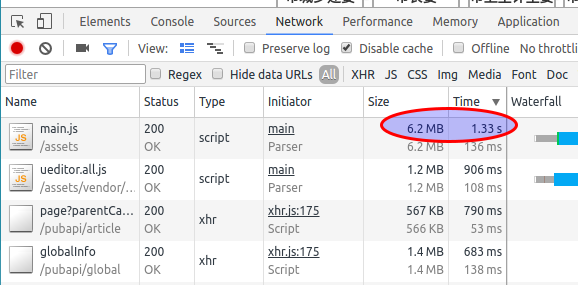
\includegraphics[scale=0.5]{largejavasript.png}
	\caption{较大的Javascript脚本}
	\label{fig:largejavasript}
\end{figure}

\subparagraph{去掉Javascript注释}

在webpack.config.js文件的plugins数组里面添加及配置插件即可。

\begin{lstlisting}[language=Javascript]
new UglifyJsPlugin({
	output: {
		comments: false,//去掉Javascript中的注释
	},
	compress: {
		warnings: false
	}
})
\end{lstlisting}

去掉注释后小了400KB左右,但是还是有6MB,没有从根本上解决问题。

\subparagraph{添加插件}

添加一些插件压缩包。

\begin{lstlisting}[language=Javascript]
plugins: [
	// <-- key to reducing React's size
	new webpack.DefinePlugin({ 
		'process.env': {
			'NODE_ENV': JSON.stringify('production')
		}
	}),
	//dedupe similar code
	new webpack.optimize.DedupePlugin(),
	//minify everything  
	new webpack.optimize.UglifyJsPlugin(), 
	//Merge chunks
	new webpack.optimize.AggressiveMergingPlugin() 
]
\end{lstlisting}


\subparagraph{React切换到产品环境}

\subparagraph{查看Webpack输出}

最最直接的,可以直接阅读Webpack的输出,里面有模块的文件大小,在package.json文件中添加--display-chunks参数,配置如下:

\begin{lstlisting}[language=Javascript]
"scripts": {
	"dev": "webpack --display-chunks --watch --progress --colors --display-error-details --config webpack/dev.config.js",
}
\end{lstlisting}


输出如图\ref{fig:webpackcheckingfilesize}所示。也可以在输出中查找是否包含重复依赖。

\begin{figure}[htbp]
	\centering
	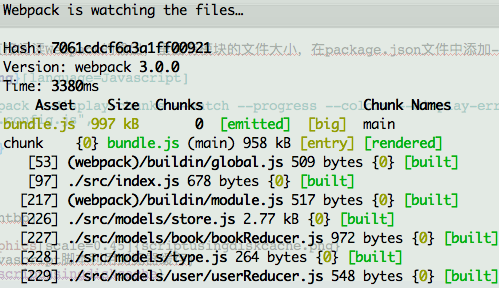
\includegraphics[scale=0.7]{webpackcheckingfilesize.png}
	\caption{Webpack查看输出文件大小}
	\label{fig:webpackcheckingfilesize}
\end{figure}


\subparagraph{利用浏览器缓存}

有时优化之后Javascript的大小还是不够理想,此时可以考虑将Javascript的文件名用Hash进行标识,Hash是经过文件计算出来的唯一值,在文件有改动后,会自动更新,浏览器仅仅在首次请求时下载较大的Javascript脚本,以后就可以直接利用本地缓存。此种方式不需要频繁的访问服务器下载Javascript脚本,提升 本地加载速度的同时也减轻了服务端的压力,如图\ref{fig:scriptusingdiskcache}所示。

\begin{figure}[htbp]
	\centering
	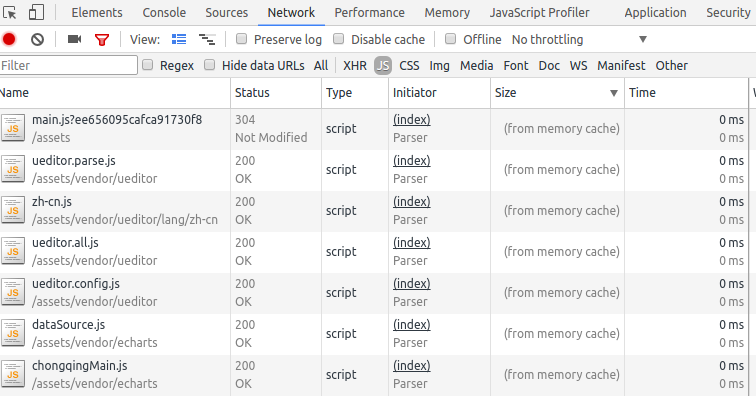
\includegraphics[scale=0.45]{scriptusingdiskcache.png}
	\caption{Javascript脚本利用浏览器缓存}
	\label{fig:scriptusingdiskcache}
\end{figure}

由于应用是SPA(Single Page Application),上图中单单一个main.js脚本都会有5MB之巨,加上其他的大大小小的Javascript脚本,在未经过服务端压缩的情况下会有10MB以上的大小,在普通的网络环境下肯定是非常慢。如果下载速度时1MB/s,打开应用至少需要10s,将是用户无法忍受的。

\subparagraph{开启Gzip压缩}

同时可以考虑在服务端开启Gzip压缩,開啓Gzip壓縮配置如下:

\begin{lstlisting}[language=Bash]
#僅僅開啓Gzip還不行,需要各項詳細配置
gzip on;
gzip_min_length 1k;
gzip_buffers 4 16k;
gzip_comp_level 2;
gzip_types application/javascript application/json text/plain application/x-javascript text/css application/xml text/javascript application/x-httpd-php image/jpeg image/gif image/png;
gzip_vary off;
gzip_disable "MSIE [1-6]\.";
\end{lstlisting}

开启服务端压缩后效果非常显著,如图\ref{fig:openservercompress}所示。

\begin{figure}[htbp]
	\centering
	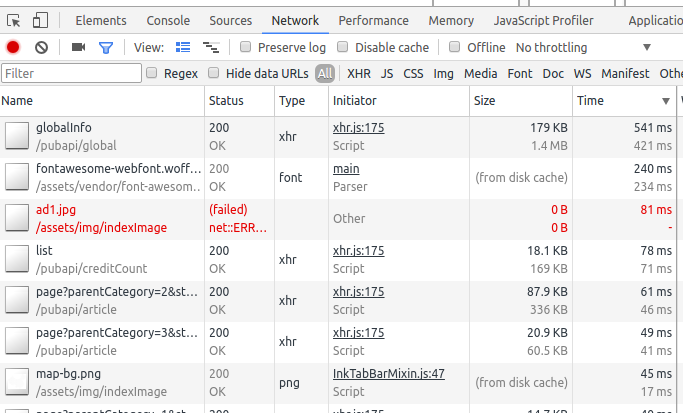
\includegraphics[scale=0.5]{openservercompress.png}
	\caption{开启服务端压缩效果}
	\label{fig:openservercompress}
\end{figure}

图中,globalInfo请求,压缩之前返回的Json有1.4MB大小,压缩之后只有179KB,压缩之前传输时间在1.5s左右,压缩之后传输时间缩短了三分之二。另外比较大的6MB的Javascript脚本也变成了1.2MB大小。

\paragraph{字体文件加载}

發現一個字體文件(fontawesome-webfont.woff2)在Linux下的Chrone中是從磁盤中加載(from disk cache)的,花費了220ms左右。在Windows平臺下的360浏览器中是從内存中加載(from cache)的。diskCache顾名思义,就是将资源缓存到磁盘中,等待下次访问时不需要重新下载资源,而直接从磁盘中获取,它的直接操作对象为CurlCacheManager。它与memoryCache最大的区别在于,当退出进程时,内存中的数据会被清空,而磁盘的数据不会,所以,当下次再进入该进程时,该进程仍可以从diskCache中获得数据,而memoryCache则不行。diskCache与memoryCache相似之处就是也只能存储一些派生类资源文件。它的存储形式为一个index.dat文件,记录存储数据的url,然后再分别存储该url的response信息和content内容。Response信息最大作用就是用于判断服务器上该url的content内容是否被修改。

\paragraph{耗时长的请求}

查看首页中一个耗时最长的请求,一般情况下耗时都稳定在1s左右。如图\ref{fig:longtimerequest}所示。可以看出挂起(stalled)304ms,等待服务端响应581ms,此两项的时间是最长的。Stalled从HTTP连接建立到请求能够被发出送出去(真正传输数据)之间的时间花费。包含用于处理代理的时间,如果有已经建立好的连接,这个时间还包括等待已建立连接被复用的时间。挂起时间长是由于浏览器对同一个主机域名的并发连接数有限制,因此如果当前的连接数已经超过上限,那么其余请求就会被阻塞,等待新的可用连接;此外脚本也会阻塞其他组件的下载。另外在不同的平台上挂起时间时长也不一定,在Windows平台的360浏览器上挂起时长(stalled)仅仅为0.458ms。

\begin{figure}[htbp]
	\centering
	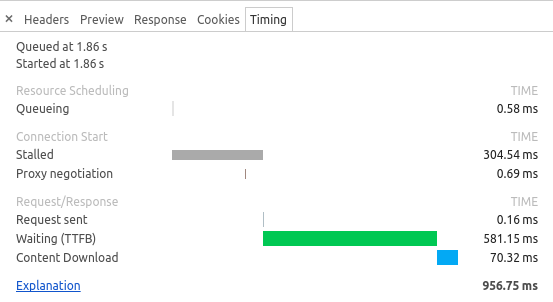
\includegraphics[scale=0.6]{longtimerequest.png}
	\caption{耗时长的请求}
	\label{fig:longtimerequest}
\end{figure}

针对服务器端耗时长的请求,使用VisualVM查看服务端调用的耗时最长的方法。VisualVM 是一款免费的性能分析工具。它通过 jvmstat、JMX、SA(Serviceability Agent)以及 Attach API 等多种方式从程序运行时获得实时数据,从而进行动态的性能分析。同时,它能自动选择更快更轻量级的技术尽量减少性能分析对应用程序造成的影响,提高性能分析的精度。

\subsection{Session}

当浏览器第一次请求时,服务器创建一个session对象,同时生成一个sessionId,并在此次响应中将sessionId 以响应报文的方式传回客户端浏览器内存或以重写url方式送回客户端,来保持整个会话。关闭此浏览器窗口,其内存中的sessionId也就随之销毁。session.invalidate()是将session设置为失效,一般在退出时使用,但要注意的是:session失效的同时 浏览器会立即创建一个新的session的,你第一个session已经失效了 所以调用它的getAttribute方法时候一定会抛出NullPointerException。jsessionid只是tomcat中对session id的叫法,在其它容器里面,不一定就是叫jsessionid。


\section{PAC(Proxy Auto-Configuration)}

\subsection{PAC简介(Pac Introduce)}

PAC是proxy auto-config的缩写。PAC文件是纯文本格式的,实际上就是JavaScript文件。PAC最简单的格式就是包含一个叫FindProxyForURL的JavaScript函数,IE通过传入两个变量来调用这个函数。一个是用户流量的地址的URL全路径,一个是这个URL中的主机名host。在日常生活中浏览器中设置代理很简单,但是当你来回切换时总是觉得很烦,你可以使用pac脚本自动判断是否走代理,方便省去了来回手动切换的烦恼。

\subsection{PAC实例(PAC Example)}

一个最简单的PAC脚本:

\begin{lstlisting}[language=JavaScript]
function FindProxyForURL(url,host){
	return "DIRECT";
}
\end{lstlisting}

参数url是用户输入的url,参数host是url中的主机名。PAC文件返回值有三种类型:

\begin{itemize}
	\item{DIRECT直连不通过代理}
	\item{PROXY www.lybbn.cn:8080 http通过8080端口代理上网,也可以使用ip:port的形式}
	\item{SOCKS5 www.lybbn.cn:8080 socks通过8080端口代理上网,可以使用ip:port形式}
\end{itemize}

\begin{lstlisting}[language=VBScript]
var FindProxyForURL = function(init, profiles) {
	return function(url, host) {
		"use strict";
		var result = init, scheme = url.substr(0, url.indexOf(":"));
		do {
			result = profiles[result];
			if (typeof result === "function") result = result(url, host, scheme);
		} while (typeof result !== "string" || result.charCodeAt(0) === 43);
			return result;
		};
		}("+dolphin2", {
		"+dolphin2": function(url, host, scheme) {
			"use strict";
			if (/^59\.214\.215\.6$/.test(host)) return "+dolphin-proxy";
			if (/^10\.10\.1\.11$/.test(host)) return "+dolphin-proxy";
			return "DIRECT";
		},
		"+dolphin-proxy": function(url, host, scheme) {
		"use strict";
		if (/^127\.0\.0\.1$/.test(host) || /^::1$/.test(host) || /^localhost$/.test(host)) return "DIRECT";
		return "PROXY 10.55.10.2:8888";
	}
});
\end{lstlisting}

以上脚本说明,当IP为58.214.215.*或10.10.1.11时,使用代理dolphin-proxy,而代理dolphin-proxy设置的是代理机器的相关信息,代理机器的IP为10.55.10.2,代理的端口是8888。

\subsection{同时连接内外网}

有时需要同时连接内网和互联网(内网与互联网不互通),开发环境需要依赖内网,与同事交流、查询资料等需要依赖互联网,而内网与互联网切换是一大痛点,不仅影响效率,同时也影响心情,宝贵的时间就在这样无意义的开关中白白浪费掉了。同时使用有线网卡和无线网卡,既能保证内网访问的安全,又能避免频繁切换网卡带来的时间开销,可谓一举两得。一般的计算机有有线网卡,也有无线网卡。一般情况下要么使用有线网卡,要么使用无线网卡,在使用无线时,连接上了有线,因为有线网卡的优先级高,故此时仅有有线能够工作,无线网卡可连接但是无法传送数据。实现双网卡的基本思路是删除默认网关,配置各自的网关即可。

\paragraph{Mac同时连内网外网}

输入如下命令查看Mac的所有网络连接方式:

\begin{lstlisting}[language=Bash]
networksetup -listallnetworkservices
\end{lstlisting}

输出的结果如下:

\begin{lstlisting}
An asterisk (*) denotes that a network service is disabled.
Apple USB Ethernet Adapter
Wi-Fi
Bluetooth PAN
Thunderbolt Bridge
\end{lstlisting}

可以看出Mac可以通过Wi-Fi联网,也可以通过USB有线联网。给指定的网络连接方式设定DNS服务器代码如下:

\begin{lstlisting}[language=Bash]
sudo networksetup -setdnsservers AirPort 192.168.10.200
\end{lstlisting}

清空DNS缓存代码如下:

\begin{lstlisting}[language=Bash]
dscacheutil –flushcache
\end{lstlisting}

输入如下命令查看MacBook的路由表:

\begin{lstlisting}[language=Bash]
netstat -nr
\end{lstlisting}

\paragraph{Fedora、Ubuntu同时连接内外网}

给有线网卡配置地址信息时,内网网卡不要加默认网关,外网网卡加默认网关,并查看无线网卡分配到的地址信息中是否有默认网关。在这里内网通过网线连接,是有线网络,外网通过无线网卡连接路由器,是无线网络。使用route命令查看默认路由(在Mac下使用netstate -nr命令),输出如图\ref{fig:routetable}所示:

\begin{figure}[htbp]
	\centering
	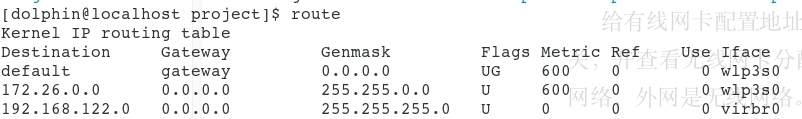
\includegraphics[scale=0.5]{route-table.jpg}
	\caption{查看Linux Kernel路由表}
	\label{fig:routetable}
\end{figure}

IP路由选择主要完成以下这些步骤:
1)搜索路由表,寻找能与目的IP地址完全匹配的表目(网络号和主机号\footnote{当前使用的IP地址有4个字节(32bit)组成,即IPV4编码方式。每个IP地址包括两部分:网络号和主机号。当分配给主机号的二进制位越多,则能标识的主机数就越多,相应地能标识的网络数就越少,反之同理。}都要匹配)。如果找到,则把报文发送给该表目指定的下一站路由器或直接连接的网络接口(取决于标志字段的值)。
2) 搜索路由表,寻找能与目的网络号相匹配的表目。如果找到,则把报文发送给该表目指定的下一站路由器或直接连接的网络接口(取决于标志字段的值)。目的网络上的所有主机都可以通过这个表目来处置。例如,一个以太网上的所有主机都是通过这种表目进行寻径的。这种搜索网络的匹配方法必须考虑可能的子网掩码。
3)搜索路由表,寻找标为“默认(default)”的表目。如果找到,则把报文发送给该表目指定的下一站路由器。如果上面这些步骤都没有成功,那么该数据报就不能被传送。如果不能传送的数据报来自本机,那么一般会向生成数据报的应用程序返回一个“主机不可达”或 “网络不可达”的错误。
完整主机地址匹配在网络号匹配之前执行。只有当它们都失败后才选择默认路由。默认路由,以及下一站路由器发送的ICMP间接报文(如果我们为数据报选择了错误的默认路由),是IP路由选择机制中功能强大的特性。

其中wlp3s0是无线网卡的名称,此命名规范为v197\footnote{https://www.freedesktop.org/wiki/Software/systemd/PredictableNetworkInterfaceNames/},说明此时的默认路由是无线网卡的路由。Destination指定该路由属于哪个网络,Gateway指定网络目标定义的地址集和子网掩码可以到达的前进或下一跃点IP地址,metric设置路由跳数,metric值越高,优先级越低。添加-p(permanent)参数永久保存此条路由信息,系统重启后路由也规则也不会丢失。flag的含义如表\ref{table:flagmeaning}所示。

\begin{table}
	\begin{center}
		\caption{flag含义}
		\bigskip
		\label{table:flagmeaning}
		\begin{tabular}{cp{10cm}c}
			\hline
			\multirow{1}{*}{序号}
			& \multicolumn{1}{c}{名称}  \\
			\hline			
			U  & Up表示此路由当前为启动状态 \\	
			H & Host,表示此网关为一主机 \\
			G & Gateway,表示此网关为一路由器\\
			R & Reinstate Route,使用动态路由重新初始化的路由\\
			D & Dynamically,此路由是动态性地写入\\
			M & Modified,此路由是由路由守护程序或导向器动态修改\\
			! & 表示此路由当前为关闭状态\\
			\hline
		\end{tabular}
	\end{center}
\end{table}

删除默认网关的命令如下:

\begin{lstlisting}[language=Bash]
# 在Windows下增加路由
route print
route -p add 10.55.10.0 mask 255.255.255.0 10.55.10.1
# 在Fedora里面执此命令删除默认网关
# Fedora 24
sudo route del default
# Ubuntu 16.04 LTS中删除默认网关
# 先连接内网,删除默认网关即可内外网同时连接
# 10.55.10.1为内网默认网关
# enx000ec6c8c163为本地有线网卡的名称
# dev为随意的命名
sudo route del default gw 10.55.10.1 dev enx000ec6c8c163
\end{lstlisting}

10.45.10.1为内网的默认网关。Linux系统的route命令用于显示和操作IP路由表(show / manipulate the IP routing table)。要实现两个不同的子网之间的通信,需要一台连接两个网络的路由器,或者同时位于两个网络的网关来实现。删除一条路由:

\begin{lstlisting}[language=Bash]
sudo route del -net 192.168.122.0 netmask 255.255.255.0
\end{lstlisting}

如果默认路由是外网网关。那么只需要单独为内网设置转发特例,所有58.214.*.*开头的,全部走enp0s26u1u2:

\begin{lstlisting}[language=Bash]
sudo route add -net 58.214.0.0 netmask 255.255.255.0 gw 10.55.10.1 dev enp0s26u1u2
\end{lstlisting}

其中58.214.0.0为内网IP的起始网段,255.255.0.0为内网的子网掩码,内网网关是10.36.40.12,eth0为内网网卡的名称。路由添加最好是添加到开机启动中:

\begin{lstlisting}[language=Bash]
vim /etc/rc.local
\end{lstlisting}

%添加删除默认网关:

\begin{lstlisting}[language=Bash]
#添加默认网关
sudo route add default gw 10.55.10.1
#删除默认网关
sudo route del default gw 10.55.10.1
\end{lstlisting}

重启网络服务:

\begin{lstlisting}[language=Bash]
/etc/init.d/networking restart
\end{lstlisting}

此时可以同时访问互联网和局域网中的主机,但是无法访问A网络。访问A网络可通过局域网代理的方式访问,将局域网的一台主机作为代理服务器,本机访问局域网中的代理服务器,代理服务器再将请求转发给A网络。在本机只需要在浏览器中配置好代理服务器即可。以FireFox浏览器为例,在Preference->Advance->Network->Connection->Settings中,增加手动代理配置,地址填写代理主机的地址,端口填写8888,代理服务器运行的是Fiddler。以后,访问内网时就使用FireFox浏览器,访问外网时就使用Google Chrome浏览器。

\paragraph{SSH代理(SSH Proxy)}
\label{paragraph:sshproxy}

数据库部署在A服务器(58.214.215.*)上,而A服务器只能连接内网才能访问,每次连接数据库都需要切换网络,实在是非常不便。但是localhost可以在外网的情况下访问B机器,B机器可以访问A机器。所以考虑通过SSH代理,以B机器(10.55.10.*)为跳板,直接访问数据库服务器A。在服务器B上建立本地端口转发,本地端口转发的格式是:

\begin{lstlisting}[language=Bash]
ssh -L <local port>:<remote host>:<remote port> <SSH hostname>
\end{lstlisting}

在B服务器(10.55.10.77)上建立一个本地端口转发:

\begin{lstlisting}[language=Bash]
ssh -L 5236:58.214.215.*:5236 10.55.10.77
\end{lstlisting}

-L参数表示做本地映射端口。将本地机(客户机)的某个端口转发到远端指定机器的指定端口. 工作原理是这样的, 本地机器上分配了一个 socket 侦听 port 端口, 一旦这个端口上有了连接, 该连接就经过安全通道转发出去, 同时远程主机和 host 的 hostport 端口建立连接. 可以在配置文件中指定端口的转发. 只有 root 才能转发特权端口. 以上的语句只能在B服务器上使用,如果其他机器想将流量发送到B服务器是无法利用隧道的。在主流 SSH 实现中,本地端口转发绑定的是 loopback 接口,这意味着只有 localhost 或者 127.0.0.1 才能使用本机的端口转发 , 其他机器发起的连接只会得到“ connection refused. ”。好在 SSH 同时提供了 GatewayPorts 关键字,我们可以通过指定它与其他机器共享这个本地端口转发。

\begin{lstlisting}[language=Bash]
ssh -g -L 5236:58.214.215.*:5236 10.55.10.*
\end{lstlisting}

-g allows remote hosts to connect to local forwarded ports.  If used on a multiplexed connection, then this option must be specified on the master process.有时我们希望转发的不止一个端口,那么可以用如下的命令多端口转发:

\begin{lstlisting}[language=Bash]
ssh -g -L 5236:58.214.215.*:5236 -L 2222:58.214.215.*:22 -L 3800:58.214.215.*:3800 10.55.10.77
\end{lstlisting}

在做端口转发时,需要保证端口转发的机器(10.55.10.77)所使用的转发端口未被已经运行的程序占用。例如10.55.10.77已经运行了sshd,那么22端口就不能作为转发端口,可以选择1022等任意未被使用的端口。在连接到1022端口时,有可能提示Connection Refused,那么此时需要检查1022端口是否可以扫描到,是否打开,代理机器到防火墙是否允许1022端口到流量通过,以及代理机器1022的配置,是否已经做了到代理机器到免密登陆。最后发现改为2222端口即可。可以使用如下命令测试端口的联通:

\begin{lstlisting}[language=Bash]
# 采用222端口时,远程机器无法连接
# 暂时不清楚原因
telnet 10.77.10.55 2222
\end{lstlisting}

telnet因为采用明文传送报文,安全性不好,很多Linux服务器都不开放telnet服务,而改用更安全的ssh方式。telnet命令用于确定远程服务的状态,这里是确定远程服务器的某个端口是否能访问。以上配置在Fedora 24下工作良好。

\paragraph{Windows代理设置}

Windows下还没有尝试直接通过ssh命令来设置代理转发,Windows下的代理需要使用putty工具。假如在A机器代理,其他机器访问A机器的2222端口流量转发到B机器(103.12.30.11)的22222端口,那么putty可以作如图\ref{fig:puttyportforwarding}所示的设置。

\begin{figure}[htbp]
	\centering
	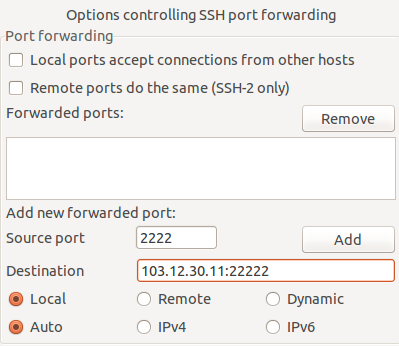
\includegraphics[scale=0.6]{puttyportforwarding.png}
	\caption{Windows下设置SSH端口转发}
	\label{fig:puttyportforwarding}
\end{figure}

当访问A机器的2222端口时,流量会自动转发到B机器的22222端口。在设置后,一段时间后会提示network error software caused connection abort。在putty的Connection选项里,选择每隔一定事件发送空的数据包来保持连接(Sending of null packets to keep session alive)。使用如下命令查看Windows端口是状态:

\begin{lstlisting}[language=Bash]
netstat -ano|findstr "3800"
\end{lstlisting}

设置好后,始终需要在前端运行一个界面。不是非常方便,所以可以让putty运行在后台。


\paragraph{SSH反向代理(Reverse Proxy)}

A网络有一台内网主机AH(A Host),可以连接互联网,有一台A网络的外网主机,无法连接互联网。此时我们可以使用SSH反向代理的方式,将A网络的外网主机端口映射到AH主机的端口。首先在AH主机上执行如下命令:

\begin{lstlisting}[language=Bash]
ssh -NfR 1234:localhost:2223 user1@123.123.123.123 -p2221
\end{lstlisting}

这句话的意思是将AH主机的1234端口和B主机的2223端口绑定,相当于远程端口映射(Remote Port Forwarding)。

\newpage
~\vfill

\part{Engneering}

\section{通用规范}

\subsection{版本管理}

在项目的开发过程中,要求有明确的版本号,以前只是在正式发布版本的时候才会生成带版本号的文件,目前测试需要每次发布版本修改时定义版本号,方便测试进行问题识别。以前直接使用脚本生成的带有年月日的版本标志,但是还是需要进一步规范化。由于发布采用的自动化脚本,在启动程序时需要指定明确的文件名称,文件名称与版本号有关联,所以考虑将版本号保存到一个文件里面,使用Gradle构建程序和发布程序时都读取此文件中的版本号。Given a version number MAJOR.MINOR.PATCH, increment the:

\begin{itemize}
	\item{MAJOR version when you make incompatible API changes,}
	\item{MINOR version when you add functionality in a backwards-compatible manner}
	\item{PATCH version when you make backwards-compatible bug fixes.}
\end{itemize}

Additional labels for pre-release and build metadata are available as extensions to the MAJOR.MINOR.PATCH format.在项目的根目录下新建version.properties文件,文件中定义版本号:

\begin{lstlisting}
VERSION_CODE=1.0.2
\end{lstlisting}

在Gradle中读取版本号:

\begin{lstlisting}
version = getVersionCode()

def getVersionCode() {
	def versionFile = file('/Users/dolphin/source/credit-system/gradle/version.properties')
	if (versionFile.canRead()) {
		def Properties versionProps = new Properties()
		versionProps.load(new FileInputStream(versionFile))
		def versionCode = versionProps['VERSION_CODE'].toString()
		/*def runTasks = gradle.startParameter.taskNames        //仅在assembleRelease任务是增加版本号
		if ('assembleRelease' in runTasks) {
			versionProps['VERSION_CODE'] = (++versionCode).toString()
			versionProps.store(versionFile.newWriter(), null)
		}*/
		return versionCode
		} else {
		throw new GradleException("Could not find version.properties!")
	}
}
\end{lstlisting}

此处文件路径写的是绝对路径,如果仅仅在本机进行构建问题不大,但是一般都是团队协作,不同的成员使用的操作系统有区别,项目存放的路径也不一样,所以写成相对路径会比较妥当。可以写成如下:

\begin{lstlisting}
File versionFile = file("$rootDir/cc-web-boot/src/main/resource/version.properties")
\end{lstlisting}

其中\$rootDir表示项目的根目录,比如有一个叫做dolphin的项目,那么rootDir就是dolphin目录,另外还有一个projectDir的变量和buildDir的变量。projectDir就是dolphin/src目录,buildDir就是dolphin/src/build目录。如果是多个Project组成的项目,那么projectDir就是rootDir/projectName,buildDir就是dolphin/projectName/build。

\subsection{项目发布(Publish)}

在项目的版本管理上,可以引进Alpha、Beta、Pre-release和Release的机制。自动发布、灰度发布、自动回滚等。

\paragraph{撰写Change Log}

在项目管理平台(禅道、Readmine等)上新建版本号,便于测试小组做测试。根据git log,生成项目的修改记录,前提是git log需要有编写规范。或者手动编写项目的修改记录,一般为优化(Optimize)、修改(Modify)、新特性(Feature)、bug修复(Bugfix)等。

\paragraph{同步数据库(Sync Database)}

将涉及到本次发布的需要添加的字段、表等等在生产环境添加。这里就需要在开发时,记录修改数据库的SQL脚本,发布时执行脚本即可。

\paragraph{打标签(Tag)}

将此次发布的正式版本打上标记(tag),一般的命名是版本号加上特点,例如1.1.35版本的,便于以后的Hotfix。

\paragraph{发布程序(Publish)}

需要注意的是,发布程序之前需要先备份原有的程序,便于回滚出现问题的版本。根据程序规模的大小,具体情况视主机的数量而定,使用脚本自动发布或者手动拷贝发布程序。

\paragraph{发布后确认}

验证发布功能是否生效。在没有接口版本管理的情况下,告知调用接口方。

%----------------------------------------------------------------------------------------
%	BIBLIOGRAPHY
%----------------------------------------------------------------------------------------

\chapter*{Bibliography}
\addcontentsline{toc}{chapter}{\textcolor{ocre}{Bibliography}}
\section*{Books}
\addcontentsline{toc}{section}{Books}
\printbibliography[heading=bibempty,type=book]
\section*{Articles}
\addcontentsline{toc}{section}{Articles}
\printbibliography[heading=bibempty,type=article]

%----------------------------------------------------------------------------------------
%	INDEX
%----------------------------------------------------------------------------------------

\cleardoublepage
\phantomsection
\setlength{\columnsep}{0.75cm}
\addcontentsline{toc}{chapter}{\textcolor{ocre}{Index}}
\printindex

%----------------------------------------------------------------------------------------

\end{document}
